\documentclass{article}
%\documentclass[]{article}
% if you need to pass options to natbib, use, e.g.:
% \PassOptionsToPackage{numbers, compress}{natbib}

% to compile a preprint version, e.g., for submission to arXiv, add
% add the [preprint] option:
\usepackage[preprint]{jmlr2e}

\usepackage{natbib}
% to avoid loading the natbib package, add option nonatbib:
% \usepackage[nonatbib]{nips_2018}

%\usepackage[backslant]{aurical}       % Fontauri fonts 
\usepackage{bm}
\usepackage[utf8]{inputenc} % allow utf-8 input
%\usepackage[T1]{fontenc}    % use 8-bit T1 fonts
\usepackage{hyperref}       % hyperlinks
\usepackage{url}            % simple URL typesetting
\usepackage{booktabs}       % professional-quality tables
\usepackage{amsfonts}       % blackboard math symbols
\usepackage{nicefrac}       % compact symbols for 1/2, etc.
\usepackage{microtype}      % microtypography
\usepackage{subfig}
\usepackage{tabularx}
\usepackage{amsmath}
\usepackage{enumerate}
\usepackage{xcolor}
%\usepackage{graphicx}
\usepackage[font=small]{caption}
%\usepackage[labelformat = empty,position=top]{subcaption}
\usepackage[export]{adjustbox}
%\usepackage[]{algorithm2e}
\usepackage{algorithm}
\usepackage{algorithmic}
\usepackage{float}
\usepackage{placeins}
\usepackage{multirow}

%  Environments

\newenvironment{itemize*}{
\begin{itemize}
\setlength{\parskip}{0em}
\setlength{\topparskip}{0em}
}
{\end{itemize}}

\newenvironment{enumerate*}{
\begin{enumerate}
\setlength{\parskip}{0em}
\setlength{\topparskip}{0em}
}
{\end{enumerate}}


% Commands
\newcommand{\comment}[1]{}
\newcommand{\techreport}[1]{#1}
%\newcommand{\mmp}[1]{}
\newcommand{\hanyuz}[1]{}
%\newcommand{\skcomment}[1]{}
\newcommand{\mmp}[1]{\textcolor{red}{#1}}
\newcommand{\skcomment}[1]{({\color{blue}{SK's comment:}} \textbf{\color{blue}{#1}})}
%\newcommand{\hanyuz}[1]{({\color{brown}{Hanyuz's comment:}} \textbf{\color{brown}{#1}})}

\newcommand{\beq}{\begin{equation}}
\newcommand{\eeq}{\end{equation}}
\newcommand{\beqa}{\begin{eqnarray}}
\newcommand{\eeqa}{\end{eqnarray}}
\newcommand{\beqas}{\begin{eqnarray*}}
\newcommand{\eeqas}{\end{eqnarray*}}

\newcommand{\bit}{\begin{itemize}}
\newcommand{\eit}{\end{itemize}}
\newcommand{\bits}{\begin{itemize*}}
\newcommand{\eits}{\end{itemize*}}
\newcommand{\benum}{\begin{enumerate}}
\newcommand{\eenum}{\end{enumerate}}
\newcommand{\benums}{\begin{enumerate*}}
\newcommand{\eenums}{\end{enumerate*}}
\newcommand{\mybullet}{$\bullet$}

%\newcommand{\BlackBox}{\rule{1.5ex}{1.5ex}}  % end of proof

% names

\newcommand{\dpullalg}{{\sc PullBackDPhi}}
\newcommand{\projg}{{\sc ProjectG}}
\newcommand{\glassoalg}{{\sc GroupLasso}}
\newcommand{\embedalg}{{\sc EmbeddingAlg}}
\newcommand{\flassoalg}{{\sc GroupLasso}}
\newcommand{\flasso}{{\sc GroupLasso}}
\newcommand{\svd}{{\sc SVD}} % to be replaced with \flassoalg !!
\newcommand{\LEalg}{{\sc LaplacianEigenmaps}}
\newcommand{\rmalg}{{\sc RMetric}}
\newcommand{\lapalg}{{\sc Laplacian}}
\newcommand{\tppalg}{{\sc LocalPCA}}
\newcommand{\ouralg}{{\sc ManifoldLasso}}


\newcommand{\srdata}{{\bf SwissRoll}}
\newcommand{\redata}{{\bf RigidEthanol}}
\newcommand{\ethdata}{{\bf Ethanol}}
\newcommand{\toldata}{{\bf Toluene}}
\newcommand{\maldata}{{\bf Malonaldehyde}}

%  math mode commands

\newcommand {\argmax}[2]{\mbox{\raisebox{-1.7ex}{$\stackrel{\textstyle
 {\rm #1}}{\scriptstyle #2}$}}\,}
\newcommand{\nchoosem}[2]{\left(\!\!\!\begin{array}{c}#1\\#2\end{array}\!\!\!\right)}  % use \binom{}{} instead
\newcommand{\fracpartial}[2]{\frac{\partial #1}{\partial  #2}}

\newcommand{\bigOO}{{\cal O}}
\newcommand{\dataset}{{\cal D}}
\newcommand{\onevector}{{\mathbf 1}}
\newcommand{\rrr}{{\mathbb R}}

\newcommand{\M}{{\cal M}}
\newcommand{\T}{{\cal T}}
%\newcommand{\S}{{\cal S}}
\newcommand{\txim}{\ensuremath{\T_{\xi_i}\M}} % tangent subspace
\newcommand{\tphim}{\ensuremath{\T_{\phi(\xi_i)}\phi(\M)}} % tangent subspace in phi(M)
\newcommand{\I}{{\cal I}} % set of indices for which to compute gradients

\newcommand{\G}{{\cal G}} % dictionary
\newcommand{\neigh}{{\cal N}}
\newcommand{\X}{{\cal X}}
\newcommand{\xb}{\mathbf{X}}  % matrices for glasso
\newcommand{\tilx}{\tilde{x}}
%\newcommand{\g}{\Fontauri{g}} % R metric as a form Fontauri not working!
\newcommand{\g}{\mathbf{g}} % R metric as a form
%\newcommand{\id}{\Fontauri{id}} % induced Euclidean metric as a form
\newcommand{\id}{\mathbf{id}} % induced Euclidean metric as a form


\newcommand{\proj}{\operatorname{Proj}}
\newcommand{\trace}{\operatorname{trace}}
\newcommand{\rank}{\operatorname{rank}}
\newcommand{\range}{\operatorname{span}}
\newcommand{\rowrange}{\operatorname{rowspan}}
\newcommand{\diag}{\operatorname{diag}}
\newcommand{\grad}{\operatorname{grad}}
\newcommand{\supp}{\operatorname{supp}}

\newcommand{\barbx}{\bar{\bar{X}}}
\newcommand{\bhat}{\hat{\beta}}
\newcommand{\zhat}{\hat{z}}
\newcommand{\barw}{\bar{\epsilon}}
\newcommand{\bbar}{\bar{\beta}}


% Theorems, etc

%\newtheorem{lemma}{Lemma}
%\newtheorem{definition}[lemma]{Definition}
%\newtheorem{proposition}[lemma]{Proposition}
%\newtheorem{theorem}[lemma]{Theorem}
%\newtheorem{corollary}[lemma]{Corollary}




\newlength{\llw}
\setlength{\llw}{\linewidth}
\newlength{\picwi}

\begin{document}

%\title{A regression approach for explaining manifold embedding coordinates}
\title{Manifold Coordinates with Physical Meaning}

% The \author macro works with any number of authors. There are two
% commands used to separate the names and addresses of multiple
% authors: \And and \AND.
%
% Using \And between authors leaves it to LaTeX to determine where to
% break the lines. Using \AND forces a line break at that point. So,
% if LaTeX puts 3 of 4 authors names on the first line, and the last
% on the second line, try using \AND instead of \And before the third
% author name.

\author{\name Samson J. Koelle${}^1$ \email sjkoelle@uw.edu \\
       \name Hanyu Zhang${}^1$ \email hanyuz6@uw.edu \\
       \name Marina Meil\u{a}${}^{1,2}$ \email mmp@stat.washington.edu \\
       \name Yu-Chia Chen${}^2$ \email yuchaz@uw.edu \\
       \addr ${}^1$Department of Statistics\\
       University of Washington\\
       Seattle, WA 98195-4322, USA   \\
       ${}^2$Department of Electrical and Computer Engineering \\
       University of Washington \\
       Seattle, WA 98195, USA
       }
       
\editor{Francis Bach, David Blei, and Bernhard Sch{\"o}lkopf}
%\author{
%  Marina Meila\thanks{\texttt{www.stat.washington.edu/mmp}}
  %\And
 % Samson Koelle \\
  %Department of Statistics\\
 % University of Washington\\
 % Seattle, WA 98195-4322 \\
  %\texttt{\{mmp2,sjkoelle,hanyuz6\}@uw.edu} \\
  %\And
  %Hanyu Zhang
%  \And
%  Yu-Chia Chen\\
   %% \And
  %% Coauthor \\
  %% Affiliation \\
  %% Address \\
  %% \texttt{email} \\
  %% \AND
  %% Coauthor \\
  %% Affiliation \\
  %% Address \\
  %% \texttt{email} \\
  %% \And
  %% Coauthor \\
  %% Affiliation \\
  %% Address \\
  %% \texttt{email} \\
  %% \And
  %% Coauthor \\
  %% Affiliation \\
  %% Address \\
  %% \texttt{email} \\
%}

\maketitle
\begin{abstract}
Manifold embedding algorithms map high-dimensional data down to
coordinates in a much lower-dimensional space. One of the aims of
dimension reduction is to find {\em intrinsic coordinates} that
describe the data manifold. The coordinates returned by the
embedding algorithm are abstract, and finding their physical or
domain-related meaning is not formalized and left to domain
experts. This paper studies the problem of recovering the
meaning of the new low-dimensional representation in a
 semi-automatic, principled fashion.  We propose a method to explain
embedding coordinates of a manifold as {\em non-linear} compositions
of functions from a user-defined dictionary. We show that this problem
can be set up as a sparse {\em linear Group Lasso} recovery problem,
find sufficient recovery conditions, and demonstrate its effectiveness
on data.

\end{abstract}

\begin{keywords}
Dimension reduction, manifold learning, functional regression, gradient, group lasso
\end{keywords}

Manifold learning algorithms, also known as embedding algorithms, map
data from high or infinite-dimensional spaces down
to coordinates in a much lower-dimensional space. In the sciences, one
of the goals of dimension reduction is the discovery of descriptors of
the data generating process. Both linear dimension reduction
algorithms like Principal Component Analysis (PCA) and non-linear algorithms
such as Diffusion Maps \citep{coifman:06} are used in applications from genetics to astronomy to uncover the variables describing
large-scale properties of the interrogated system.

For example, in chemistry, a common objective is to discover so-called
{\em collective coordinates} describing the evolution of molecular
configurations at long time scales, which correspond to
macroscopically interesting transformations of the molecule, and can
explain some of its
properties \citep{clementiOnuchicNymeyer:00,Noe2017-up}.
Figure \ref{fig:molecs} illustrates how manifold learning is used for this purpose. In {\em Molecular Dynamics (MD) simulations}, a molecular configuration is represented by the $3N_a$ vector of spatial locations of the $N_a$ atoms comprising the molecule. A MD simulation produces a sample of molecular configurations; the distribution of this sample describes the molecule's behavior in the given experimental conditions. It has been shown empirically that manifolds  approximate these high-dimensional distributions \citep{Dsilva13-Nonlinear}. 

Figure \ref{fig:toluene-bonds} shows the toluene molecule, consisting of $N_a=15$ atoms, and \ref{fig:tol_circ} shows the mapping of an MD simulated trajectory into $m=2$ dimensions (the embedding coordinates) by a manifold learning algorithm. Visual inspection shows that this configuration space is well-approximated by a one-dimensional manifold parametrized by a geometric quantity, the {\em torsion} $g_1$ of the methyl bond, which is the angle formed by the planes inscribing the first three and last three atoms of the colored lines joining four atoms in Figure \ref{fig:tol_circ}. Thus, $g_1$ is a collective coordinate describing the "slow motions'' of the toluene molecule, filtered out from the faster modes of vibration by the manifold learning algorithm. 
%
\begin{figure}[htb]
\subfloat[][Toluene]{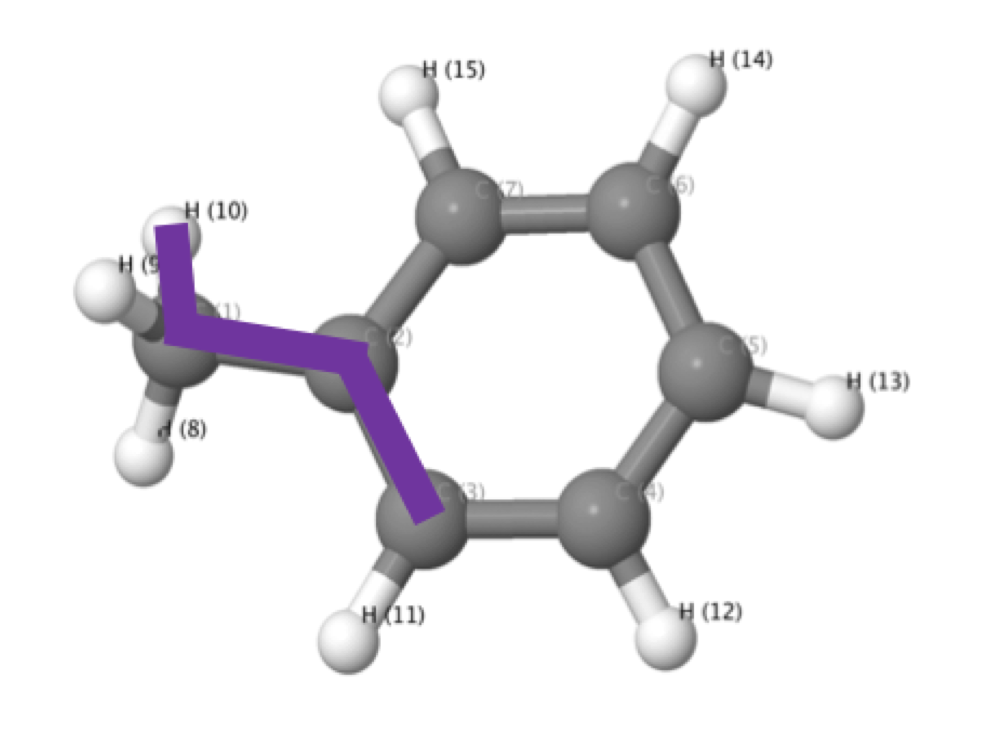
\includegraphics[width=3cm, height=3cm, trim={-.5cm, -.5cm,
-.5cm, -.5cm}, clip]{../Figures/tolbonds}\label{fig:toluene-bonds}}\hfill
\subfloat[][Ethanol]{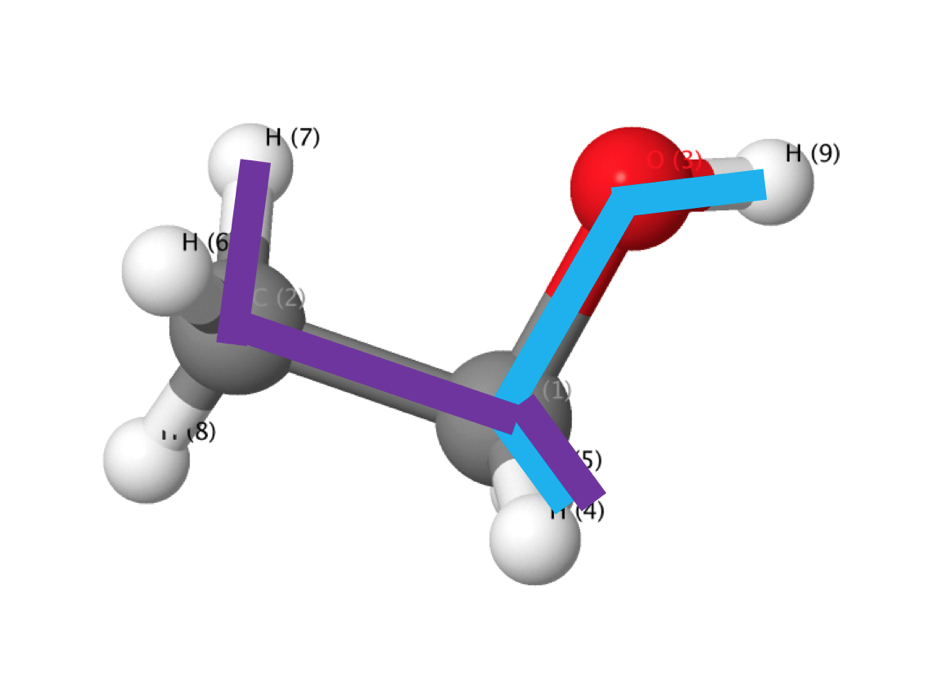
\includegraphics[width=3cm, height=3cm, trim={-1cm, -1cm,
-1cm, -1cm}, clip]{../Figures/ethbonds}\label{fig:ethanol-bonds}}\hfill
\subfloat[][Malonaldehyde]{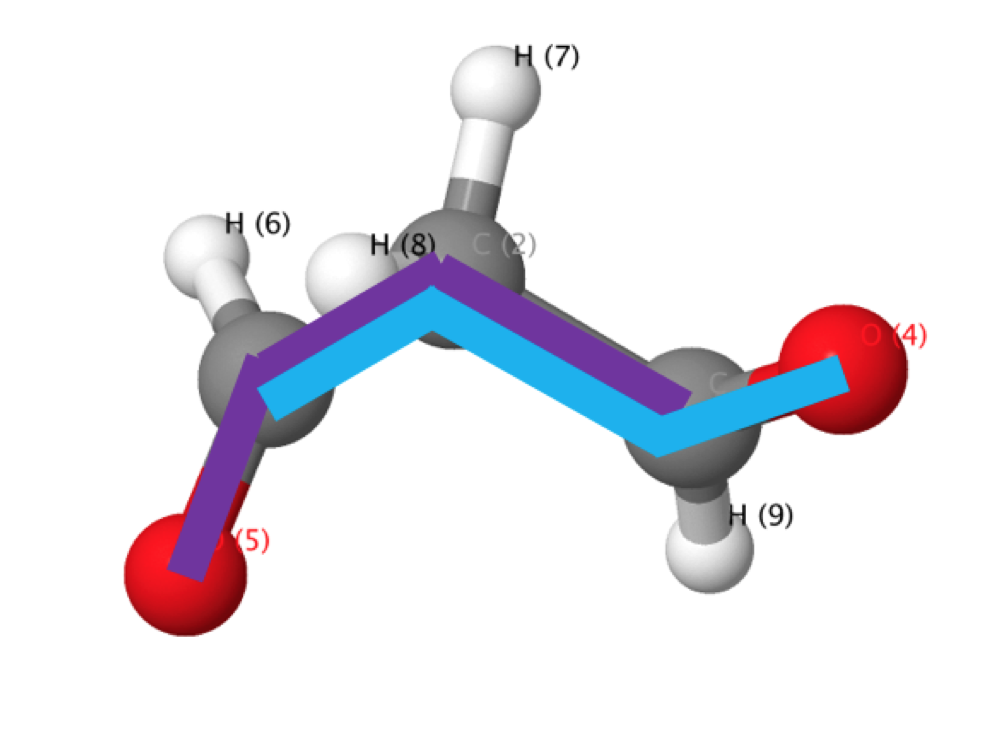
\includegraphics[width=3cm, trim={0, -3cm, 0, 0},
clip]{../Figures/malbonds}\label{fig:mda-bonds}}\hfill \newline
\subfloat[][$g_1$]{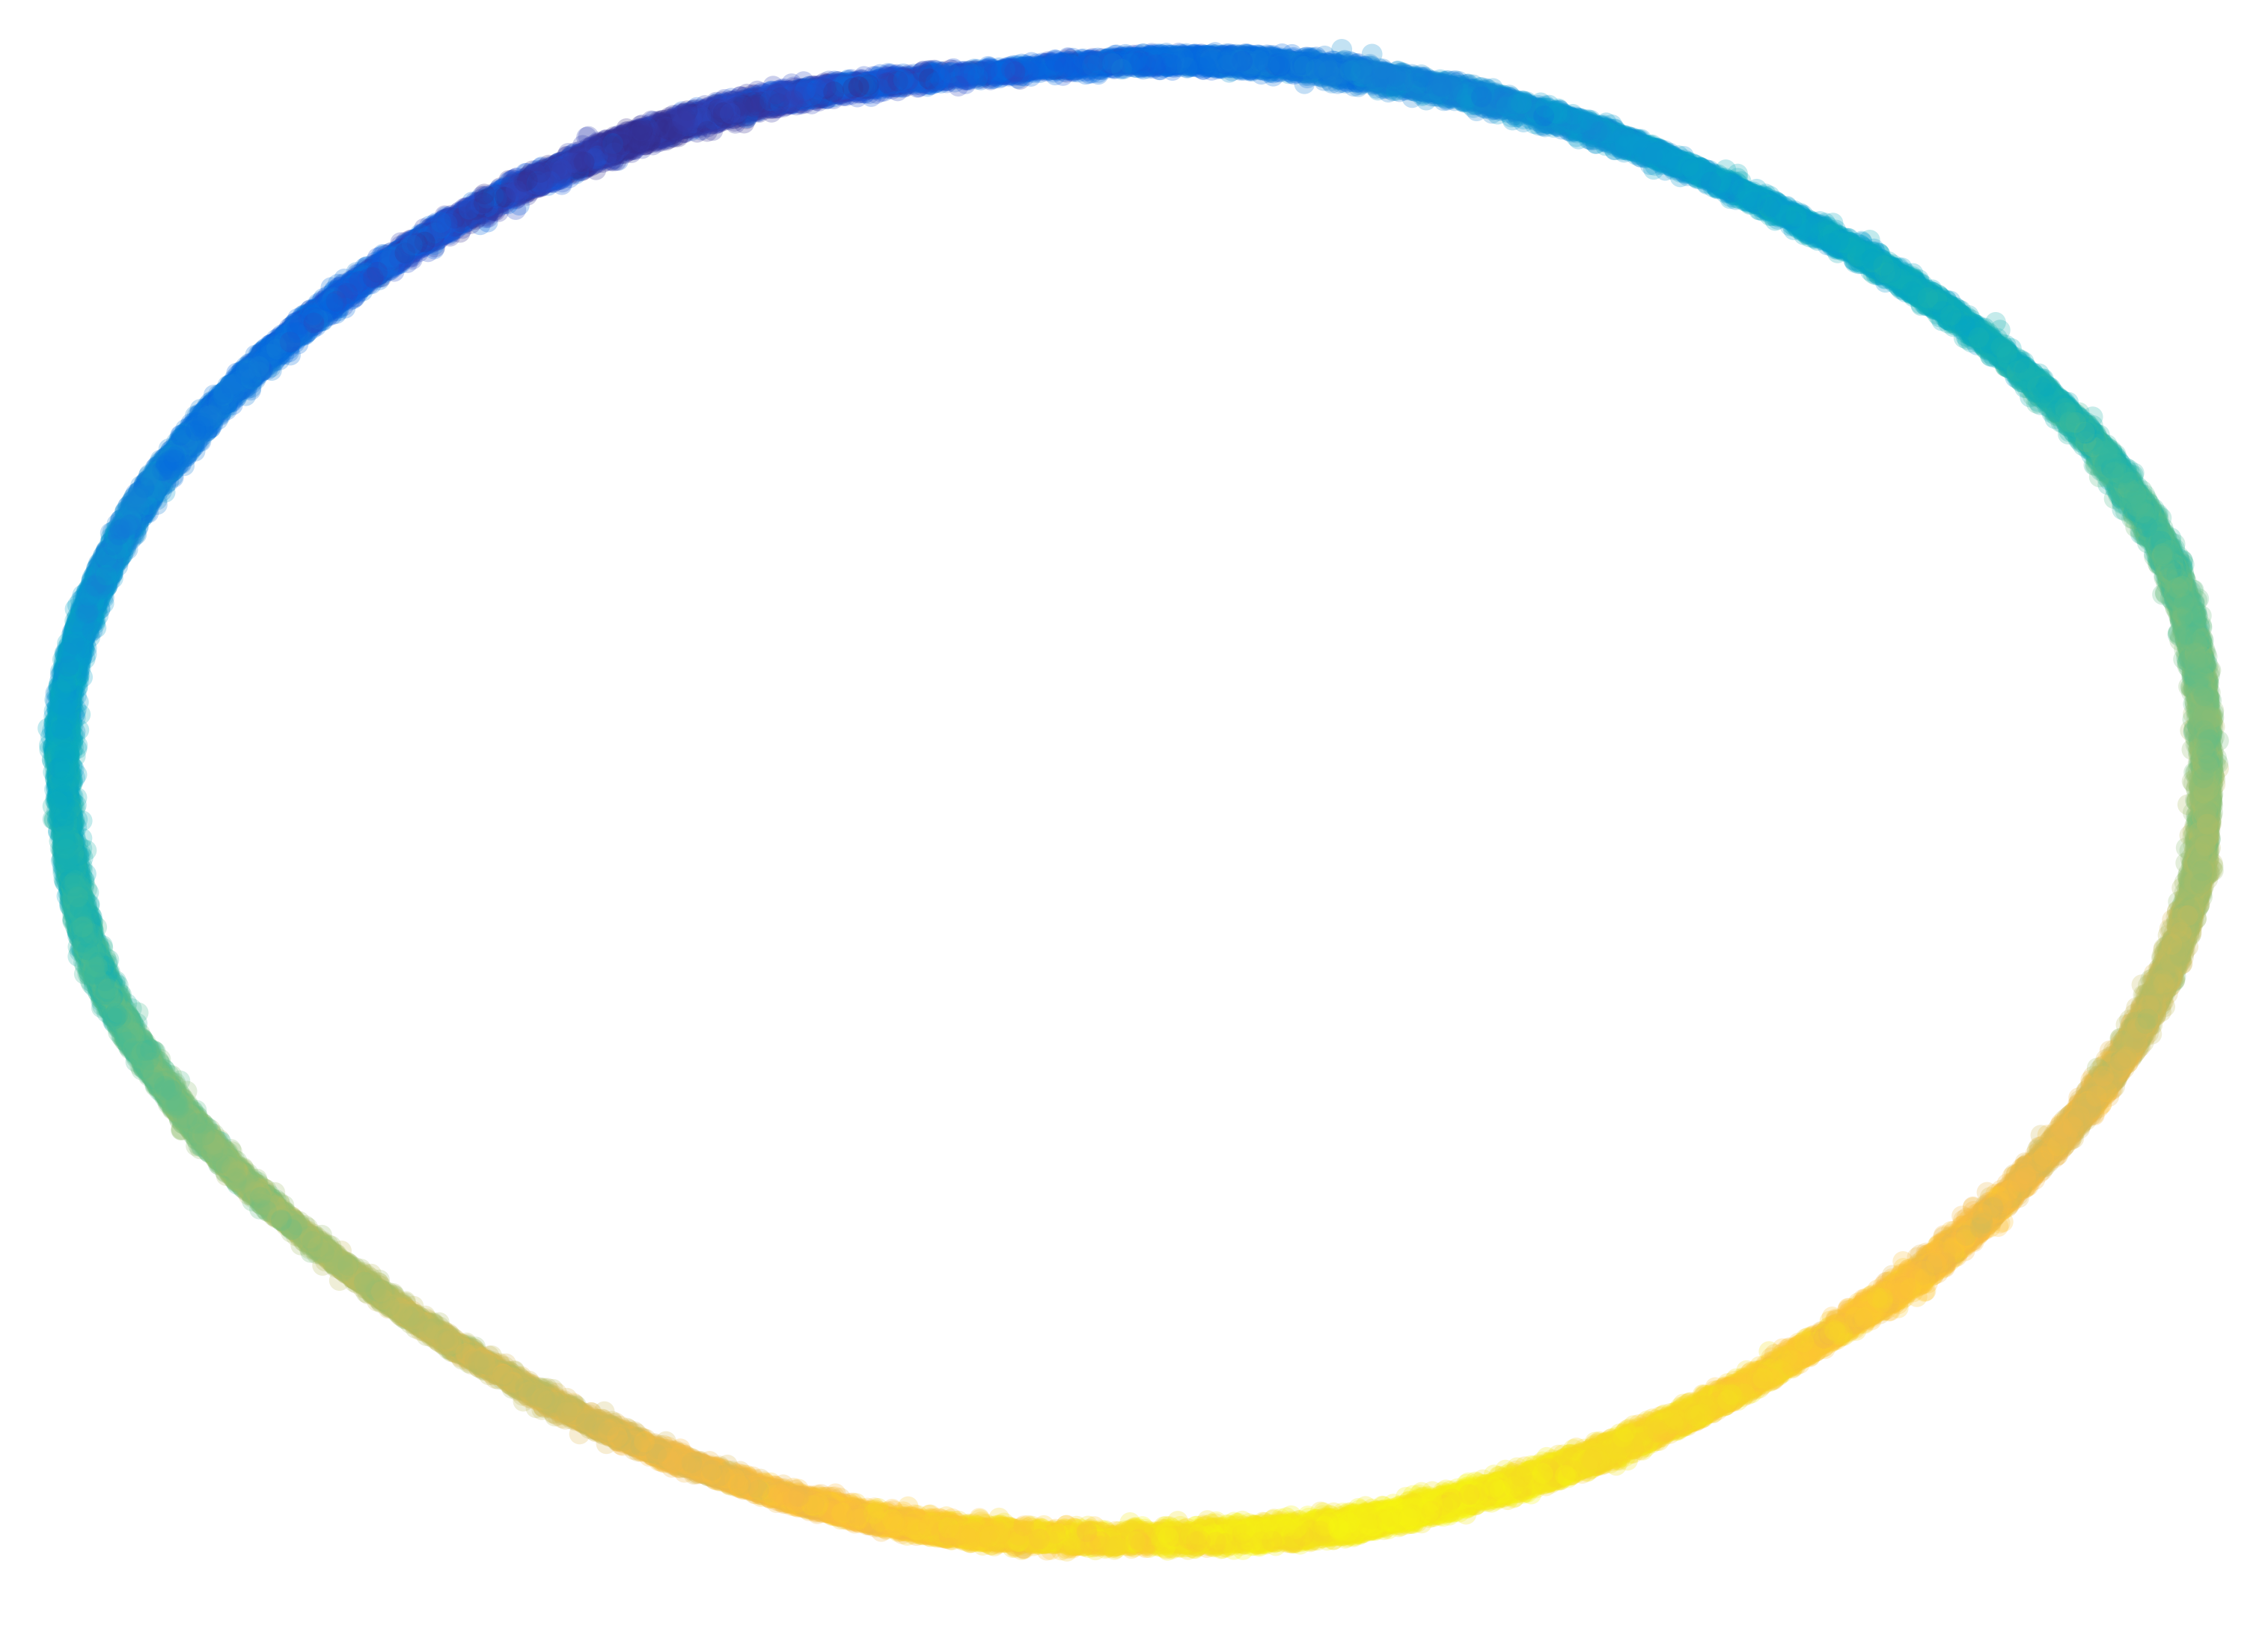
\includegraphics[width=3cm, height=3cm, trim={-1cm, -1cm,
-1cm, -1cm}, clip]{../Figures/toluene-embedding-deformation-torsion.png}\label{fig:tol_circ}}\hfill
\subfloat[][$g_1$]{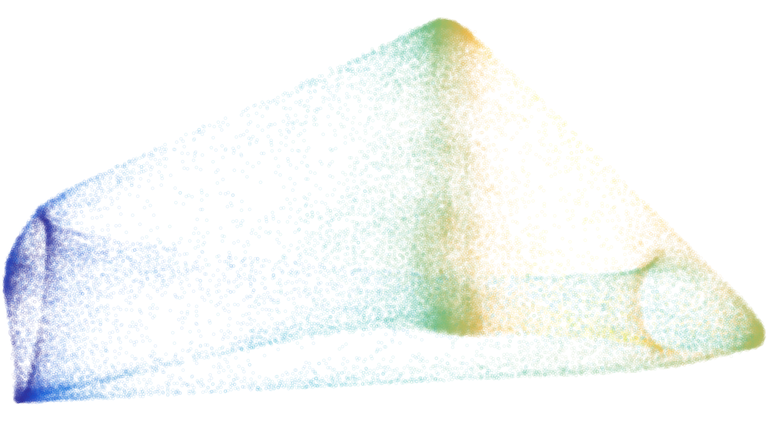
\includegraphics[width=3cm, height=3cm, trim={-1cm, -1cm,
-1cm, -1cm}, clip]{../Figures/ethanoltorsion1.png}\label{fig:eth_tor1}}\hfill
\subfloat[][$g_1$]{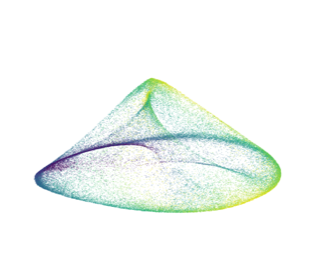
\includegraphics[width=3cm, trim={.5cm, .5cm,
.5cm, .5cm},
clip]{../Figures/malonaldehyde/g1.png}\label{fig:mal_tor1}}\hfill \newline
\subfloat[][Torsion example]{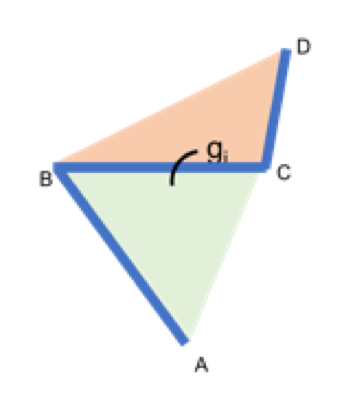
\includegraphics[width=3cm, trim={.5cm, .5cm,
.5cm, .5cm},
clip]{../Figures/torsionexplain.png}\label{fig:tor_explain}}\hfill 
%\hbox to 60.0mm{}
\subfloat[][$g_2$]{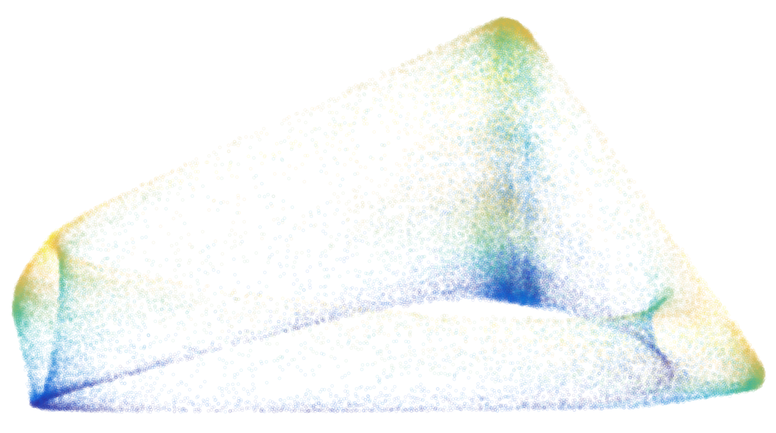
\includegraphics[width=3cm, height=3cm, trim={-1cm, -1cm,
-1cm, -1cm}, clip]{../Figures/ethanoltorsion2.png}\label{fig:eth_tor2}}\hfill
\subfloat[][$g_2$]{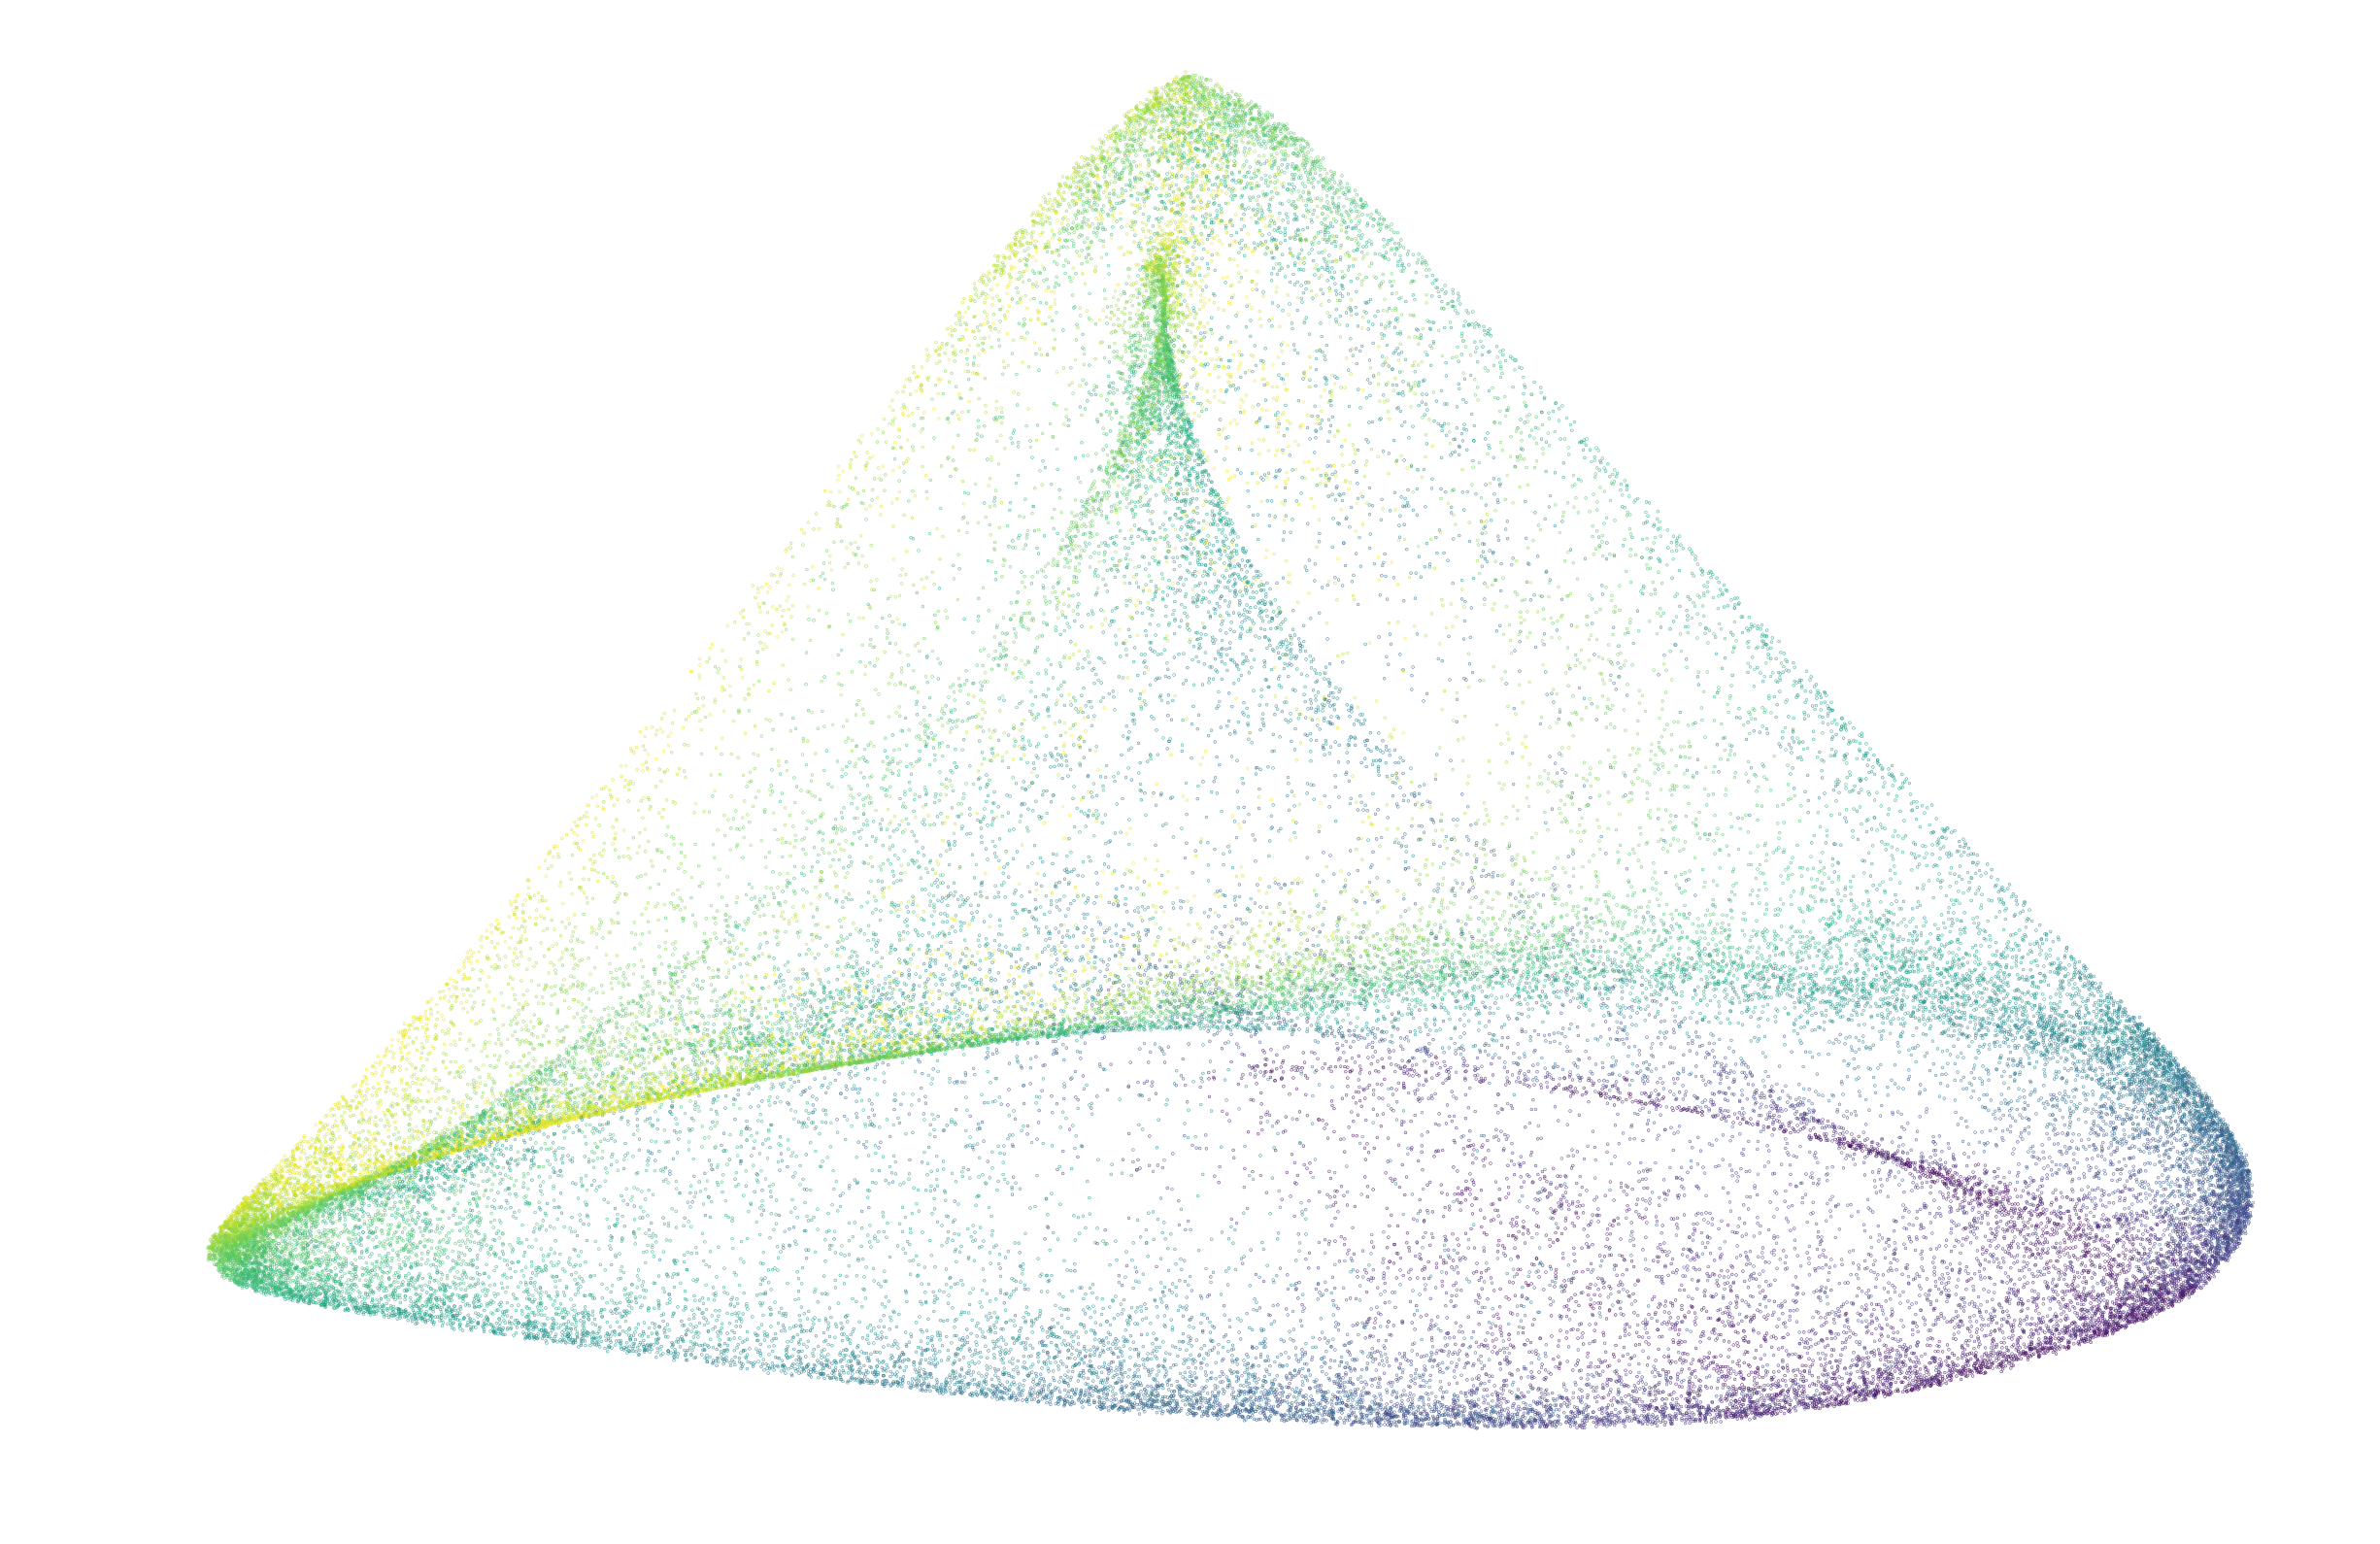
\includegraphics[width=3cm, trim={0, -3cm, 0, 0},
clip]{../Figures/malonaldehyde/April_01_2019_22_23_48/embeddingpic2.png}\label{fig:mal_tor2}}\hfill 
\caption{Collective coordinates with physical meaning in Molecular Dynamics (MD) simulations. \ref{fig:toluene-bonds}-\ref{fig:mda-bonds} Diagrams of the toluene ($C_7 H_8$), ethanol ($C_2H_5OH$), and malonaldehyde ($C_3H_4O_2$) molecules, with the carbon (C) atoms in grey, the oxygen (O) atoms in red, and the hydrogen (H) atoms in white. Bonds defining important torsions $g_j$ are marked in purple and blue  (see Section \ref{sec:exps} for more details). The bond torsion is the angle of the planes inscribing the first three and last three atoms on the line (\ref{fig:tor_explain}).  \ref{fig:tol_circ} Embedding of the configurations of toluene into $m=2$ dimensions, showing a manifold of $d=1$. The color corresponds to the values of the purple torsion $g_1$. \ref{fig:eth_tor1}, \ref{fig:eth_tor2} Embedding of the configurations of the ethanol in $m=3$ dimensions, showing a manifold of dimension $d=2$, respectively colored by the blue and purple torsions in Figure \ref{fig:ethanol-bonds}. \ref{fig:mal_tor1}, \ref{fig:mal_tor2}. Embedding of the configurations of the malonaldehyde in $m=3$ dimensions, showing a manifold of dimension $d=2$, respectively colored by the blue and purple torsions in Figure \ref{fig:mda-bonds}.}
    \label{fig:molecs}
%, as follows: in \ref{fig:toluene-bonds} the purple torsion represents the rotation of the $CH_3$ {\em methyl} group, relative to the $C_6H_5$ {\em benzene} group; in \ref{fig:ethanol-bounds} the purple torsion represents the rotation of the methyl group relative to the middle $CH_2$ group, and the blue torsion the rotation of the $OH$ {\em hydroxyl} group relative to the same $CH_2$ group; in \ref{fig:mda-bonds}, the two torsions respectively represent the rotation of the left and right $CO$ {\em carbonyl} groups relative to the central $CH_2$ group. 
\end{figure}
%

While embedding algorithms are able to uncover the manifold structure of these data, finding the physical meaning of the 1D manifold coordinate in Figure \ref{fig:tol_circ} was done by visual inspection. In general, a trained human expert would scan through many torsions and other functions of the configuration, in order to find ones that can be identified with the abstract coordinates output by a PCA or ML algorithm. Manual inspection of denoised coordinates for features of interest is pervasive in a variety of scientific fields \citep{Chen2016-eq, Herring2018-cq}. The goal of this paper is to put this process on a formal basis and to devise a method for automating this identification, thus removing the time consuming visual inspections from the shoulders of the scientist. We introduce a method to semi-automatically establish relationships of the meaningless abstract coordinates output by an embedding algorithm with functions of the data that are meaningful or interesting in the domain of the problem.

In our paradigm, the scientist inputs a {\em dictionary} $\G$
of functions to be considered as possible collective coordinates. For the examples
in Figure \ref{fig:molecs}, $\G$ could be a set of candidate
torsions. We propose an algorithm that recovers a set of functions
$g_1,\ldots g_s\in\G$, so that $(g_{1:s})$ is a local diffeomorphism
to the output of the embedding algorithm; in other words, so that
$(g_{1:s})$ are collective coordinates for the manifold. To keep the approach as
general as possible, we do not rely on a particular embedding
algorithm, making only the minimal assumption that it produces a
smooth embedding. We also do not assume a parametric relationship
between the embedding and the functions in the dictionary $\G$. Hence,
we only assume that the mapping between the data manifold and the
functions is sufficiently smooth. 

Our method is to compose differentials of functional covariates to
reconstruct the differentials of the manifold embedding coordinates, and is
therefore robust to non-linearity in both the algorithm and the
functional covariates. In other words, by considering differentials,
we map our original non-linear, non-parametric problem to a 
linear sparse regression.

The next section defines the problem formally,
and Section \ref{sec:background} presents the necessary background in manifold
estimation. Section \ref{sec:ouralg} develops our method, \ouralg.  
The relationship to previous work is discussed in
Section \ref{sec:related}. Section \ref{sec:theory} presents theoretical recovery results,  Section \ref{sec:exps} presents experiments, and Section \ref{sec:conc} concludes the paper. The Appendices present details of the functional dictionaries used as well as the adaptions necessary to make our method work in the rotation and translation invariant molecular configuration space.


\section{Problem formulation, assumptions and challenges}
\label{sec:problem}
We make the standard assumption that the observed data
$\dataset=\{\xi_i \in \rrr^D : i \in 1 \dotsc n\}$ are sampled
i.i.d. from a {\em smooth manifold} \footnote{The reader is referred
  to \citet{smoothmfd} for the definitions of the differential
  geometric terms used in this paper.} $\M$ of intrinsic dimension $d$
embedded in $\rrr^D$ by the inclusion map. In this
paper, we will call {\em smooth} any function or manifold of class at
least ${\cal C}^3$. The precise notion of {\em near} varies with
  the embedding approach, and is beyond the scope of this paper. We
assume that the intrinsic dimension $d$ of $\M$ is known; for example,
by having been estimated previously by one method in
\citet{Kleindessner2015DimensionalityEW}. The manifold $\M$ is a {\em
  Riemannian manifold} with {\em Riemannian metric} inherited from the
ambient space $\rrr^D$. Furthermore, we assume the existence of a
smooth {\em embedding map} $\phi:\M\rightarrow \phi(\M)\subset\rrr^m$,
where typically $m << D$.  That is, $\phi$ restricted to $\M$ is
  a diffeomorphism onto its image, and $\phi(M)$ is a submanifold of
  $\rrr^m$.  We call the coordinates $\phi(\xi_i)$ in this $m$
dimensional ambient space the {\em embedding coordinates}; let $\Phi =
[\phi(\xi_i)^T]_{i=1:n} \in \mathbb R^{n\times m}$.  In practice, the
mapping of the data $\dataset$ onto $\phi(\dataset)$ represents the
output of an embedding algorithm, and we only have access to $\M$ and
$\phi$ via $\dataset$ and its image $\phi(\dataset)$.

In addition, we are given a {\em dictionary} of user-defined and domain-related smooth functions $\G=\{g_1,\ldots g_p,\,\text{with }g_j: U \subseteq \rrr^D \rightarrow \rrr\}$. Our goal is to express the embedding coordinate functions 
$\phi_1 \dotsc \phi_m$ in terms of functions in $\G$.

More precisely, we assume that
$\phi(x)=h(g_{j_1}(x),\ldots\,g_{j_s}(x))$, where $h:O\subseteq
\rrr^s\rightarrow \rrr^m$ is a smooth function of $s$ variables, defined
on a open subset of $\rrr^s$ containing the ranges of
$g_{j_1},\ldots\,g_{j_s}$. Let $S=\{{j_1},\ldots\,{j_s}\}$, and
$g_S=[g_{j_1}(x),\ldots\,g_{j_s}(x)]^T$. The problem is to discover the
set $S\subset [p]$ such that $\phi=h\circ g_S$. We call $S$ the {\em
  functional support} of $h$, or the {\em explanation} for the
manifold $\M$ in terms of $\G$. For instance, in the toluene
example, the functions in $\G$ are all the torsions in the
molecule, $s=1$, and $g_S=g_1$ is the explanation for the
1-dimensional manifold traced by the configurations.

\paragraph{Indeterminacies}
In differential geometric terms, the explanation $g_S$ is strongly related to finding {\em coordinate systems}, {\em charts}, and {\em parameterizations} of $\M$.
Since the function $\phi$ given by the embedding algorithm is not unique, the function $h$ cannot be uniquely determined. For the same reason, it would be overly restrictive to assume a parametric form for $h$. Hence, this paper aims to find the support set $S$ circumventing the identification of $h$. We leave to future work the problem of recovering information on how the functions $g_S$ combine to parameterize $\M$.

Indeterminacies w.r.t. the support $S$ itself are also possible. For instance, the support $S$ may not be unique whenever the relationship  $g_1=t(g_2)$, where $t$ is a smooth monotonic function, holds for two functions in $\G$.
 In Section \ref{sec:theory}
we give conditions under which $S$ can be
recovered uniquely; intuitively, they consist of functional
independencies between the functions in $\G$. For instance, it is
sufficient to assume that that the dictionary $\G$ is a {\em
  functionally independent} set, i.e. there is no $g\in \G$ that can be
obtained as a smooth function of other functions in $\G$. 

\section{Problem formulation, assumptions and challenges}
%\label{sec:problem}
We make the standard assumption that the observed data
$\dataset=\{\xi_i \in \rrr^D : i \in 1 \dotsc n\}$ are sampled
i.i.d. from a {\em smooth manifold} \footnote{The reader is referred
  to \citet{smoothmfd} for the definitions of the differential
  geometric terms used in this paper.} $\M$ of intrinsic dimension $d$
embedded in $\rrr^D$ by the inclusion map. In this
paper, we will call {\em smooth} any function or manifold of class at
least ${\cal C}^3$. The precise notion of {\em near} varies with
  the embedding approach, and is beyond the scope of this paper. We
assume that the intrinsic dimension $d$ of $\M$ is known; for example,
by having been estimated previously by one method in
\citet{Kleindessner2015DimensionalityEW}. The manifold $\M$ is a {\em
  Riemannian manifold} with {\em Riemannian metric} inherited from the
ambient space $\rrr^D$. Furthermore, we assume the existence of a
smooth {\em embedding map} $\phi:\M\rightarrow \phi(\M)\subset\rrr^m$,
where typically $m << D$.  That is, $\phi$ restricted to $\M$ is
  a diffeomorphism onto its image, and $\phi(M)$ is a submanifold of
  $\rrr^m$.  We call the coordinates $\phi(\xi_i)$ in this $m$
dimensional ambient space the {\em embedding coordinates}; let $\Phi =
[\phi(\xi_i)^T]_{i=1:n} \in \mathbb R^{n\times m}$.  In practice, the
mapping of the data $\dataset$ onto $\phi(\dataset)$ represents the
output of an embedding algorithm, and we only have access to $\M$ and
$\phi$ via $\dataset$ and its image $\phi(\dataset)$.

In addition, we are given a {\em dictionary} of user-defined and domain-related smooth functions $\G=\{g_1,\ldots g_p,\,\text{with }g_j: U \subseteq \rrr^D \rightarrow \rrr\}$. Our goal is to express the embedding coordinate functions 
$\phi_1 \dotsc \phi_m$ in terms of functions in $\G$.

More precisely, we assume that
$\phi(x)=h(g_{j_1}(x),\ldots\,g_{j_s}(x))$, where $h:O\subseteq
\rrr^s\rightarrow \rrr^m$ is a smooth function of $s$ variables, defined
on a open subset of $\rrr^s$ containing the ranges of
$g_{j_1},\ldots\,g_{j_s}$. Let $S=\{{j_1},\ldots\,{j_s}\}$, and
$g_S=[g_{j_1}(x),\ldots\,g_{j_s}(x)]^T$. The problem is to discover the
set $S\subset [p]$ such that $\phi=h\circ g_S$. We call $S$ the {\em
  functional support} of $h$, or the {\em explanation} for the
manifold $\M$ in terms of $\G$. For instance, in the toluene
example, the functions in $\G$ are all the torsions in the
molecule, $s=1$, and $g_S=g_1$ is the explanation for the
1-dimensional manifold traced by the configurations.

\paragraph{Indeterminacies}
In differential geometric terms, the explanation $g_S$ is strongly related to finding {\em coordinate systems}, {\em charts}, and {\em parameterizations} of $\M$.
Since the function $\phi$ given by the embedding algorithm is not unique, the function $h$ cannot be uniquely determined. For the same reason, it would be overly restrictive to assume a parametric form for $h$. Hence, this paper aims to find the support set $S$ circumventing the identification of $h$. We leave to future work the problem of recovering information on how the functions $g_S$ combine to parameterize $\M$.

Indeterminacies w.r.t. the support $S$ itself are also possible. For instance, the support $S$ may not be unique whenever the relationship  $g_1=t(g_2)$, where $t$ is a smooth monotonic function, holds for two functions in $\G$.
 In Section \ref{sec:theory}
we give conditions under which $S$ can be
recovered uniquely; intuitively, they consist of functional
independencies between the functions in $\G$. For instance, it is
sufficient to assume that that the dictionary $\G$ is a {\em
  functionally independent} set, i.e. there is no $g\in \G$ that can be
obtained as a smooth function of other functions in $\G$. 

\comment{
For example,
the toluene manifold could be equally well be parametrized by
$g_1=\cos(\tau)$ or by $g_2 = \sin \tau = \cos (\tau + \pi/2)$, or by
any other function that is related by a monotonic transformation of
its domain. The number of charts and the existence of universal
parameterizations of the manifold effect $s$ as well. \skcomment{I
  understand charts matters in some part of the theory section, but I
  am wondering why?  A torus has $s=2$ because it has a universal
  parameterization, while a sphere has $s=2$ expect at a particular
  point with no measure. A sphere has $2$ charts minimum, while a
  torus has 3 charts minimum, so what is the correspondence?}
}

\section{Manifold learning and intrinsic geometry}
\label{sec:background}
Suppose we observe data points $\xi_i \in \rrr^D$ that are sampled
from a smooth $d$-dimensional submanifold $\M \subset \rrr^D$. The
task of manifold learning is to provide a diffeomorphism $\phi: \M \to
\phi(\M) \subset \rrr^m$ where $m \ll D$. The Whitney Embedding
Theorem \citep{smoothmfd} guarantees the existence of a map satisfying this
property with $m \leq 2d$. That is, a good manifold learner will
identify a smooth map $\phi: \M \to \rrr^m$ with $d \le m \le 2d \ll
D$.

\paragraph{The neighborhood graph and kernel matrix} The {\em neighborhood graph} is a data structure that 
associates to each data point $\xi_i\in\dataset$ its set of {\em neighbors} 
$\neigh_i=\{i'\in [n], \text{with}\,||\xi_{i'}-\xi_{i}||\leq r_N\}$, 
where $r_N$ is a {\em neighborhood radius} parameter. 
The neighborhood relation is symmetric, and determines an undirected graph with nodes
 represented by the data points $\xi_{1:n}$;  $|\neigh_i|$ is  denoted by $k_i$.
 
Closely related to the neighborhood graph are the local position matrices $\Xi_i = \{\xi_{i'} : i' \in \neigh_i\} \in \rrr^{k_i \times d}$, local embedding coordinate matrices $\Phi_i = \{\phi(\xi_{i'}) : i' \in \neigh_i\} \in \rrr^{k_i \times d}$, and the {\em kernel matrix}
$K \in \rrr^{n \times n}$ whose elements are
\beq
K_{ii'}= \begin{cases} \exp\left( -\tfrac{||\xi_i-\xi_{i'}||}{\epsilon_N^2}\right)  \; &\text{ if} \;i'\in\neigh_i  \\
0 \; \text{otherwise}.
\end{cases}
\label{eq:kernelmatrix}
\eeq Typically, the radius $r_N$ and the {\em bandwidth} parameter
$\epsilon_N$ are related by $r_N=c \epsilon_N$ with $c$ a small
constant greater than 1. This ensures that $K$ is close to its limit
when $r_N\rightarrow \infty$ while remaining sparse, with sparsity
structure induced by the neighborhood graph. Rows of this matrix will be
denoted $K_{i, \neigh_i}$ to emphasize that when a particular row is
passed to an algorithm, only $k_i$ values need to be
passed. Next, we show how the neighborhood graph, local position matrices, and kernel
matrix are used in manifold estimation algorithms.


\paragraph{Estimating tangent spaces in the ambient space $\rrr^D$}
The tangent subspace at point $\xi_i$ in the data, denoted $\T_{\xi_i}\M$, can be estimated by
{\em Weighted Local Principal Component Analysis} \citep{Chen2013}, as described in the
\tppalg~algorithm. The output of this algorithm is an orthogonal matrix
$T_i\in\rrr^{D\times d}$, representing a basis for $\T_{\xi_i}\M$. For
this algorithm and others we define the SVD algorithm
$\svd(X,d)$ of a symmetrical matrix $X$ as outputting
$V,\Lambda$, where $\Lambda$ and $V$ are the largest $d$ eigenvalues
and their eigenvectors, respectively. We denote a column vector of
ones of length $k$ by $ \bm{1}_k$. 
%
\begin{algorithm}[H]
\floatname{algorithm}{\tppalg} \renewcommand{\thealgorithm}{}
\caption{(local data $\Xi_i$,  kernel row $K_{i,\neigh_i}$, intrinsic dimension $d$)}
\begin{algorithmic}[1]
\STATE Compute weighted mean $\bar \xi_i = (K_{i,\neigh_i} \bm{1}_{k_i})^{-1} K_{i,\neigh_i} \Xi_i $
  \STATE Compute weighted local difference matrix $Z_{i} = (K_{i, \neigh_i}  \bm{1}_{k_i}) ^{-1} K_{i , \neigh_i} (\Xi_i - \bm{1}_{k_i} \bar \xi_i)$
  \STATE Compute $T_i, \Lambda \leftarrow \text{SVD} (Z_i^T Z_i, d)$
  \STATE {\bf Output} $T_i$ 
\end{algorithmic}
\end{algorithm}


\paragraph{The renormalized graph Laplacian}
The {\em renormalized graph Laplacian}, also known as the {\em sample
  Laplacian}, or {\em Diffusion Maps Laplacian} $L$, constructed by the 
\lapalg~ algorithm, converges to the manifold Laplace operator
$\Delta_\M$; \citet{coifman:06} shows that this estimator is unbiased
w.r.t. the sampling density on $\M$ (see also \citet{HeinAL:05}, \citet{HeinAL:07,TingHJ:10}). The
Laplacian $L$ is a sparse matrix; row $i$ of $L$ contains non-zeros
only for $i'\in\neigh_i$. Thus, as for $K$, rows of this matrix will
be denoted $L_{i, \neigh_i}$. The sparsity pattern of $L$, too, is given by the
neighborhood graph; construction of the neighborhood graph is
therefore the computationally expensive component of this
algorithm. 

% used in section Section \ref{sec:explain-dphi} to 

%\begin{algorithm}[H]
%\floatname{algorithm}{\lapalg}
%\renewcommand{\thealgorithm}{}
%\caption{(Dataset $\dataset$, neighborhoods $\neigh_{i:n}$, bandwidth $\epsilon_N$)}
%\begin{algorithmic}[1]
%  \STATE {\bf Input} 
%  \STATE Compute kernel matrix $K$ using \ref{}
%  \STATE Compute normalization weights $w_{i}\,\gets\,  K_{i, \neigh_i} \bm{1}_{k_i} $, $w\,\gets\,\diag(w_{i} \; {i=1:n})$
%  \STATE Normalize $\tilde{L}\,\gets\, w^{-1}K $
%  \STATE Compute renormalization weights $\tilde w_i\,\gets\,  \tilde{L}_{i, \neigh_i} \bm{1}_{k_i}, \; \tilde w=\diag( \tilde w_i \;{i=1:n})$
%  \STATE Renormalize $L\,\gets\,4({\tilde w }^{-1} \tilde L -\diag(\tilde w_i)_{i=1:n})$ \skcomment{Check}
%  \STATE {\bf Output} Laplacian matrix $L$, [optionally $K$]
%\end{algorithmic}
%\end{algorithm}
%
\begin{algorithm}[H]
\floatname{algorithm}{\lapalg}
\renewcommand{\thealgorithm}{}
\caption{(neighborhoods $\neigh_{i:n}$, local data $\Xi_{1:n}$, bandwidth $\epsilon_N$)}
\begin{algorithmic}[1]
%  \STATE {\bf Input} 
  \STATE Compute kernel matrix $K$ using (\ref{eq:kernelmatrix})
  \STATE Compute normalization weights $w_{i}\,\gets\,  K_{i, \neigh_i} \bm{1}_{k_i} $, $i=1,\ldots n$,  $W\,\gets\,\diag(w_{i} \; {i=1:n})$
  \STATE Normalize $\tilde{L}\,\gets\, W^{-1}K W^{-1} $
  \STATE Compute renormalization weights $\tilde w_i\,\gets\,  \tilde{L}_{i, \neigh_i} \bm{1}_{k_i}$, $i=1,\ldots n$, $\tilde W=\diag( \tilde w_i \;{i=1:n})$
  \STATE Renormalize $L\,\gets\,\frac{4}{ \epsilon_N^2}({\tilde W }^{-1} \tilde L - I_n)$
  \STATE {\bf Output} Kernel matrix $K$, Laplacian $L$, [optionally $\tilde{w}_{1:n}$]
\end{algorithmic}
\end{algorithm}
%
The $m$ principal eigenvectors of the Laplacian $L$ (or alternatively
of the matrix $\tilde{L}$ of Algorithm \lapalg), corresponding to its
smallest non-zero eigenvalues, are sometimes used as embedding coordinates
$\Phi$ of the data; the embedding obtained is known as the {\em
  Diffusion Map} \citep{coifman:06} or the {\em Laplacian Eigenmap} \citep{belkin:01} of
$\dataset$.  We use this embedding approach for convenience, but in
general, any algorithm which asymptotically generates a smooth
embedding is acceptable.

\paragraph{The pushforward Riemannian metric} Geometric quantities such as angles and lengths of vectors in the tangent bundle $\T\M$ and distances along curves in $\M$ are captured by Riemannian geometry. We assume that $(\M,\id)$ is a {\em Riemannian manifold}, with the metric $\id$ induced from $\rrr^D$. Furthermore, we associate with $\phi(\M)$ a Riemannian metric $\g$ which preserves the geometry of $(\M,\id)$. This metric is called the {\em pushforward Riemannian metric} and is defined by
\beq \label{eq:rmetric0}
\langle u,v\rangle_{\g}\;=\;\langle D\phi^{-1}(\xi)u,D\phi^{-1}(\xi)v\rangle
\quad\text{ for all }u,v\in\T_{\phi(\xi)}\phi(\M).
\eeq
In the above, $D$ denotes the differential operator, and $D\phi^{-1}(\xi)$ is the {\em pull-back} operator, that maps vectors from $\T_{\phi(\xi)}\phi(\M)$ to $\T_\xi\M$, and $\langle , \rangle$ is the Euclidean scalar product. 

For each $\phi(\xi_i)$, the associated push-forward Riemannian metric
expressed in the coordinates of $\rrr^m$, is a symmetric,
semi-positive definite $m\times m$ matrix $G_i$ of rank $d$. The scalar product $\langle u,v \rangle_{\g}$ takes the form $u^TG_iv$.

The matrices $G_i$ can be estimated by the algorithm \rmalg~of
\citet{2013arXiv1305.7255P}. The algorithm uses only local information, and thus can be run
efficiently. For notational simplicity, we refer to the $m$ embedding
coordinates of the points in a neighborhood of a point $i$ as
$\Phi_{i}$.
%
\begin{algorithm}[H]
\floatname{algorithm}{\rmalg}
\renewcommand{\thealgorithm}{}
\caption{(Laplacian row $L_{i, \neigh_i}$, local embedding coordinates $\Phi_{i}$, intrinsic dimension $d$)}
\begin{algorithmic}[1]
\STATE Compute centered local embedding coordinates $\tilde \Phi_i \gets \Phi_{i} - \phi(\xi_i)\bm{1}_{k_i}^T  $
\STATE %$H_{ikk'}=L_{i,\neigh_i} (\tilde \Phi_{i,k} \odot \tilde \Phi_{i,k'})$ for $k,k'=1:m$.
Form matrix $H_i$ by $H_i \gets [H_{ikk'}]_{k,k' \in 1:m}$ with 
 $H_{i,kk'}=\sum_{i'\in \neigh_i}L_{i,i'}\tilde \Phi_{i,i'k} \tilde \Phi_{i,i'k'}$ for $k,k'=1:m$. 
  \STATE  Compute $V_i, \Lambda_i \gets \text{SVD} (H_i, d)$
    \STATE $G_i\,\gets\,V_i \Lambda_i^{-1} V_i^T$.
  \STATE {\bf Output} $G_i$
\end{algorithmic}
\end{algorithm}
%
%Together, these algorithms form the machinery of {\em metric learning}.


%\input{gradients-jmlr-flasso}
\section{The \ouralg~algorithm}
\label{sec:ouralg}
The main idea of our approach is to exploit the well-known mathematical fact that, for any smooth maps $f,g,h$ with
$f =h\circ g$, the differentials $Df,Dh,Dg$ at any point are in
the {\em linear} relationship $Df = Dh Dg$. 
Thus, given sets of functions $\phi_{1:m}$ and $g_{1:p}$ of a smooth manifold $\M$, we propose to recover a subset $g_{S}$ of $g_{1:p}  $ such that $\phi_{1:m} =h \circ g_S$ by solving a set of dependent linear sparse recovery problems.
Note that there is one problem for each data point, and the support is selected without explicit estimation of $h$.

The \ouralg~algorithm, the main algorithm of this paper, implements this idea.
It takes as input data $\dataset$ sampled from an unknown manifold $\M$, a dictionary $\G  = g_{1:p}$ of functions defined on $\M$ (or alternatively on an open subset of the ambient space $\rrr^D$ that contains $\M$), and an embedding $\phi(\dataset)$ in
$\rrr^m$.
The output of \ouralg~is a set $S$ of indices in $\G$,
representing the functions in $\G$ that explain $\M$. 

The first part of the algorithm calculates the necessary gradients.
This comprises Steps \ref{alg:neb}--\ref{alg:prob} and is detailed in Sections \ref{sec:grad-g} and \ref{sec:pull-back}.
For each data point, we perform several operations in the tangent subspaces $\T_{\xi_i}\M$ and $\T_{\phi(\xi_i)} \phi (\M)$.
We thus estimate orthonormal bases $T_i^\M$ and $T_i^\phi$ of these spaces using \ref{alg:tan} and \rmalg.  
Steps \ref{alg:neb} and \ref{alg:lap} consist of constructing the neighborhood graph and the kernel and Laplacian matrices that we use to compute these tangent spaces.
The gradients of the dictionary w.r.t. the manifold $\M$ are then obtained as columns of the $d\times p$ matrices $X_i$ in Steps \ref{alg:dict} and \ref{alg:dict_proj} as described in Section \ref{sec:grad-g}.
Finally, the gradients at $\xi_i$ of the coordinates $\phi_{1:m}$, also seen as functions of $\M$, are calculated as columns of the $d \times m $ matrix $Y_i$ by the \dpullalg~algorithm in Step \ref{alg:pb} as described in Section \ref{sec:pull-back}. 
%These operations are described in Section \ref{sec:grad-g}.

The second part of the algorithm, namely Step \ref{alg:glasso}, finds the support $S$ by solving a sparse regression problem; this is described in Section \ref{sec:flasso-manifold}.
In this step, a \flassoalg~algorithm is called to perform sparse regression of the manifold coordinates' gradients $Y_{1:n}$ on the gradients of the dictionary functions $X_{1:n}$.
The indices of those dictionary functions whose $\beta$ coefficients are not identically null represent the support set $\supp \beta$.
%The following section presents the main steps of the algorithm, including formal definitions of the relevant gradients.

There are several optional steps and substitutions in our algorithm.
An embedding can be computed in Step \ref{alg:embed}, or input separately by the user.
We denote this step generically as \embedalg.
Furthermore, although we explicitly describe tangent space estimation methods of both $\T_{\xi_i} \M$ and $\T_{\phi(\xi_i)} \phi (\M)$ in our algorithms, other approaches may be used as well.
Finally, scaling of functions is addressed through normalization in Section \ref{sec:ouralg-normalization}.
%In step \ref{alg:tan}, orthogonal bases of these tangent subspace are estimated by the \tppalg~algorithm described in Section \ref{sec:background}.

%
\begin{algorithm}[H]
\floatname{algorithm}{\ouralg}
\renewcommand{\thealgorithm}{}
\caption{(Dataset $\dataset$, dictionary $\G$, embedding coordinates $\phi(\dataset)$,  intrinsic dimension $d$, kernel bandwidth $\epsilon_N$, neighborhood cutoff size $r_N$, regularization parameter $\lambda$)}
\begin{algorithmic}[1]
\STATE Construct $\neigh_i$ for $i=1:n$; $i'\in \neigh_i$ iff $||\xi_{i'}-\xi_{i}||\leq r_N$, and local data matrices $\Xi_{1:n}$ \label{alg:neb}
\STATE Construct kernel matrix and Laplacian $K, L\,\gets\,$\lapalg($\neigh_{1:n},\Xi_{1:n},\epsilon_N$) \label{alg:lap}
\STATE [Optionally compute embedding: $\phi(\xi_{1:n})\gets$\embedalg$(\dataset,\neigh_{1:n},m,\ldots)$] \label{alg:embed}
  \FOR {$i=1,2,\ldots n$ (or subset) {\em (Prepare gradients for group lasso)}} 
  \STATE Compute basis  ${T_i^\M} \gets $\tppalg$(\Xi_i, K_{i, \neigh_i},d)$ \label{alg:tan}
  \STATE Compute $\nabla_\xi g_j (\xi_i)$ for $j=1,\ldots p$ \label{alg:dict}
  \STATE Project $X_i\gets {T_i^\M}^T\nabla_\xi g_{1:p}$ \label{alg:dict_proj}
  \STATE Compute $Y_i \gets$\dpullalg$(\Xi_i, \Phi_{i},T_i^\M,  L_{i, \neigh_i},  d)$ \label{alg:pb} \label{alg:prob}
  \ENDFOR
\STATE $\beta\,\gets$ \flassoalg$(X_{1:n}, Y_{1:n}, \lambda/\sqrt{mn})$ \label{alg:glasso}
\STATE {\bf Output} $S=\supp \beta$ 
\end{algorithmic}
\end{algorithm}

\subsection{Gradients and coordinate systems}
\label{sec:explain-dphi}

The \ouralg~algorithm regresses the gradients of the coordinate
functions $\phi_{1},\ldots \phi_m$ on the
gradients of the dictionary functions.
Both sets of gradients are with respect to the manifold $\M$, and so this requires calculating or estimating various gradients in the
same $d$-dimensional coordinate system.
This and the following two sections explain these procedures. 

First, note that by assumption we have two Euclidean spaces $\rrr^D$ and $\rrr^m$, in which manifolds $\M$ and $\phi(\M)$ of dimension $d$ are embedded.
Denote gradients w.r.t. the Euclidean coordinate systems in $\rrr^D$ and $\rrr^m$ by $\nabla_\xi$ and $\nabla_\phi$, respectively.
Since our interest is in functions on manifolds, we
also define the gradient of a function on a manifold $\M$.
The {\em gradient} of $f$ at $\xi$, denoted $\grad_{\M} f(\xi)\in\T_\xi\M$, is defined by $\langle \grad_{\M} f(\xi),v\rangle=Df(\xi)v$ for any $v\in \T_\xi \M$.
Denote gradients in the tangent bundles of $\M$ and $\phi(\M)$ by $\grad_\M$ and $\grad_{\phi(\M)}$, respectively. 
For each data point $\xi_i$, we will fix bases $T_i^\M$ in $\T_{\xi_i}\M$ and $T_i^\phi$ in $\T_{\phi (\xi_i)} \phi (\M)$.
Gradients expressed in these coordinate systems will be denoted by $\grad_{T_i^\M}$ and $\grad_{T_i^\phi}$ respectively.
The next section describes how to calculate dictionary gradients in the bases $T_i^\M,\,i\in[n]$.

\subsection{Calculating the gradients of the dictionary functions}
\label{sec:grad-g}

Our goal is to obtain $X_i$, the matrix containing $\grad_{T_i} g_j (\xi_i)$ as columns, where $g_j$ is a function in the dictionary $\G$.
By definition, for any basis $T_i^\M \in \rrr^{D\times d}$ of $\T_{\xi_i}\M$,
\beq
\label{eq:gradprojg} \grad_{T_i^\M}g_j(\xi_i)\;=\;T_i^T\nabla_{\xi}g_j(\xi_i).
\eeq
In other words, $\grad_{T_i^\M}g_j$ is the projection of $\nabla_\xi g_j$ on the basis $T_i^\M$.
These bases of $\T_{\xi_i}\M$, for every $i$, are estimated by \tppalg~as described in Section \ref{sec:background}.
The gradients $\nabla_\xi g_j(\xi_i)$ are known analytically, by assumption.
We thus construct matrices $X_i$, for $i=1,\ldots n$, with $p$ columns representing the gradients of the $p$ dictionary functions;
%
\beq \label{eq:X-manifold}
X_i\,=\,[\grad_{T_i^\M} g_j(\xi_i)]_{j=1:p}\,\in \rrr^{d\times p}.
\eeq
Next, we explain our estimator of $\grad_{T_i^\M} \phi_k$, the gradients of the coordinate functions.

\subsection{Estimating the coordinate gradients by pull-back}
\label{sec:pull-back}

Our goal is to obtain $Y_i$, the matrix containing $\grad_{T_i^\M}\phi_k (\xi_i)$ as columns.
Since $\phi$ is implicitly determined by a manifold embedding algorithm, the gradients of $\phi_k$ are often not analytically available, and $\phi_k$ is known only through its values at the data points.
We therefore introduce a gradient estimator based on the notion of vector-pullback between tangent spaces.

The \dpullalg~Algorithm performs gradient estimation via local linear regression in tangent spaces $\T \M$ and $\T \phi(\M)$.
%\comment{We therefore estimate these gradients by in order to define a pullback between the tangent spaces $\T \M$ and $\T \phi \M$ \cite{Luo2009-mp} \cite{2013arXiv1305.7255P}.} 
This algorithm takes as inputs the local neighborhoods $\Xi_i$ and $\Phi_i$ of points $\xi_i$ and $\phi_i$ in the original and embedding spaces, respectively, as well as bases $T_i^\M$ of $\T_{\xi_i}\M$ and $T_i^\phi$ of $\T_{\phi_i} \M$.
Estimation of $T_i^\M$ is accomplished as in the previous section, while $T_i^\phi$ is estimated via the singular vectors output by \rmalg~ \citep{2013arXiv1305.7255P} described in Section \ref{sec:background}.
%Note that both of these tangent space estimators take as input the row of the Laplacian matrix corresponding to $i$.  
Geometrically, at each data point, this algorithm first projects gradients of the coordinate functions $\nabla_{\phi} \phi_k$ onto $T_{\phi(\xi_i)} \phi(M)$ to get $\grad_{T_i^\phi} \phi_k$, and then pulls these back to $T_i^\M$ to get $\grad_{T_i^\M} \phi_k$ by solving a linear system with respect to the neighborhood.
%The idea of the algorithm is to use this correspondence in order to pull back the gradient of the coordinate function $\phi_k$ into the coordinates $T_i$.

%We , and introduce an algorithm that estimates the gradient through projection onto 

This algorithm is based on the observation that gradient estimation on a manifold is exactly the operation of vector projection and pullback between tangent spaces of isometric Riemannian manifolds.
% following observation about gradients in coordinate systems with metric.
To see this, note that in a coordinate system $T_i^\phi$, writing $\g$ in $T_i^\phi$ as $G$, we have the definition
\beq
\grad_{T_i^\phi, G} f = G^{-1} \grad_{T_i^\phi, I_d} f
\eeq
where $\grad_{T_i^\phi, I_d} f =\grad_{T_i^\phi} f =  {T_i^\phi}^T \nabla_\phi f$ is with respect to the identity metric in $\rrr^m$ \citep{Lee:03}.
Thus, since $\grad_{\phi(\M)} \phi_k \in \tphim$, by the definition of $\g$  \eqref{eq:rmetric0}, we have that
%$( \Xi_i {T_i^\M} )^T  Y_i \,=\,   \Phi_i {T_i^\phi} $ 
\beq%\label{eq:gref-diff}
(D \phi^{-1} u)^T   \grad_{T_i^\M} \phi_k  \,\approx\, u^T \grad_{T_i^\phi, I_d} \phi_k \,\quad {i'\in \neigh_i}
\eeq
where $u \in \tphim$.
In particular, note that this is invariant to $\g$.
Hence, since $T_i^\M$ and $T_i^\phi(M)$ approximate the logarithmic map to the first order with error tending to 0 within the neighborhood radius \citep{coifman:06}, we have that
\beq\label{eq:gref-diff}
((\xi_{i'}-\xi_i)^T T_i^\M)^T Y_i \,\approx\, ( \phi(\xi_{i'})-\phi(\xi_i))^T T_i^\phi \,\quad {i'\in \neigh_i}
\eeq
with
\beq \label{eq:yYbetaijk-manifold}
Y_i\,=\,[y_{ik}]_{k=1}^m\,=\,[\grad_{T_i}\phi_k(\xi_i)]_{k=1}^m\in \rrr^{d\times m}.
\eeq

As long as sufficient neighbors are present, $A$ can be made of full rank $d$, and we can obtain $Y_i$ as the least-squares solution of 
\beq\label{eq:yi-manifold2}
(\Xi_i^T T_i^\M)^T Y_i \,\approx\,  \Phi_i T_i^\phi \,\quad {i'\in \neigh_i}.
\eeq

From a statistical perspective, this method is exactly local multivariate multiple linear regression with projection onto the manifolds $\M$ and $\phi(\M)$; it is local principal components regression with the additional step of projection onto the manifold in in the embedding coordinates.
It provides an alternative approach to regularized methods such as \citet{Aswani2011-li}
 for encouraging robustness to both statistical noise around $\M$ and $\phi(\M)$ and lowering the effective dimensionality of the regression problem.
Finally, note that when $m=d$, assuming a good embedding, then $T_i^\phi = I_d$.

\begin{algorithm}[H]
\floatname{algorithm}{\dpullalg}
\renewcommand{\thealgorithm}{}
\label{alg:pullback} 
\caption{local data $\Xi_i$, local embedding coordinates $\Phi_{i}$ basis $T_i^\M$ (Optional: $T_i^\phi$ or Laplacian row $L_{i,\neigh_i}$, intrinsic dimension $d$)}
\begin{algorithmic}[1]
%  \STATE {\bf Input} .
\STATE Compute tangent space $T_i^\M \gets$ \tppalg$(( L_{i,\neigh_i}, \Xi_{i}, d)$ (Optional import).
%\STATE Compute tangent space $T_i^\phi \gets \svd (\rmalg(( L_{i,\neigh_i}, \Phi_{i}, d),d)$
  \STATE Compute pushforward metric $G_i\gets$ \rmalg$( L_{i,\neigh_i}, \Phi_{i}, d)$ (Optional import $T_i^\phi$).
  \STATE Compute $T_i^\phi, \Lambda_i= \svd(G_i, d)$. (Optional import $T_i^\phi$).
   %\STATE Project $A_i=T_i^T(\Xi_i-\xi_i\bm{1}_{k_i}^T)$.
   %\STATE Compute $B_i = \Phi_{i} - \phi(\xi_i)\bm{1}_{k_i}^T  \in\rrr^{|\neigh_i| \times m }$.
   \STATE Solve linear system $( \Xi_i {T_i^\M} )^T  Y_i \,=\,   \Phi_i {T_i^\phi} $ as in \eqref{eq:yi-manifold2}
  \STATE {\bf Output} $Y_i$ 
%  \eqref{eq:pullbacksystem}
\end{algorithmic}
\end{algorithm}

%The columns of $A_i$ and $Y_i$ are vectors in $\T_{\xi_i}\M$, the columns of $B_i$ are in $\rrr^m$ and the columns of $\tilde{B}_i$ are in $\T_{\phi(\xi_i)}\phi(\M)$.

%Of these matrices, $A_i$ and $B_i$ can be easily computed (Steps 2 and 3 of Algorithm \dpullalg), while $Y_i$ contains the gradients we want to estimate. Note that when $m=d$, $B_i=\tilde{B}_i$. These vectors are shown schematically in Figure \ref{fig:pullback}.
%where 
%\beq
%A_i\,=\,\left[{T_i^\M}^T (\xi_{i'}-\xi_i)\right]_{i'\in
 % \neigh_i} \in \rrr^{d\times k_i} ,
%B_i\,=\,\left[{T_i^\phi(M)}^T \phi(M)} \phi(\xi_{i'})-\phi(\xi_i)\right]_{i'\in \neigh_i}
%\;\in \rrr^{m\times k_i},
%\eeq
%This is a dimension-reduced adaptation of the usual linear regression formula.
%All three steps depend on the the pushforward Riemannian metric $G_i$ associated with the tangent subspace $\T_{\phi(\xi_i)}\phi(\M)$. This is estimated  using the \rmalg~algorithm  \citep{2013arXiv1305.7255P} described in Section \ref{sec:background}. For each $i$, $G_i$ is the associated push-forward Riemannian metric at $\phi(\xi_i)$,  expressed in the coordinates of $\rrr^m$ by $G_i$. This is done in Step 1 of the \dpullalg~Algorithm.

%Instead of estimating these gradients naively from differences $\phi_k(\xi_i)-\phi_k(\xi_{i'})$ between neighboring points, we first estimate their values in $\T_{\phi(\xi_i)}\phi(\M)$, then use the differential geometric notion of vector {\em pull back} to obtain them in the $T_i$ coordinate system.
%This method is novel, and is of independent interest as it allows tranformations of vector fields between non-isometric embeddings of the data. 

%We make the following notations, with $\proj_T v$ denoting the Euclidean projection of vector $v$ onto subspace $T$.
% 
%\beq
%A_i\,=\,\left[\proj_{\T_{\xi_i}\M}(\xi_{i'}-\xi_i)\right]_{i'\in
%  \neigh_i} \in \rrr^{d\times k_i} 
%\eeq
%
%\beq \label{eq:yYbetaijk-manifold}
%Y_i\,=\,[y_{ik}]_{k=1}^m\,=\,[\grad_{T_i}\phi_k(\xi_i)]_{k=1}^m\in %\rrr^{d\times m},
%\eeq
%
%and
%
%\beq 
%B_i\,=\,\left[\phi(\xi_{i'})-\phi(\xi_i)\right]_{i'\in \neigh_i}
%\;\in \rrr^{m\times k_i},
%\quad
%%\tilde{B}_i\,=\,\left[\proj_{\T_{\phi(\xi_i)}\phi(\M)}\left(\phi(\xi_{i'})-\phi(\xi_i)\right)\right]_{i'\in \neigh_i},
%\;\in \rrr^{d\times k_i}.
%\eeq

%this m = d \implies the above assumes something about the embedding...

%Moreover, the columns of $A_i$ and $\tilde{B}_i$ are in correspondence, because, to first order approximation, they represent the same vectors in two different coordinate systems, namely the {\em   logarithmic map} \citep{DoCarmo} of point $i'$ with respect to point $i$.






%If the embedding induced by $\phi$ were an isometry, the estimation of $\tphim$ could be performed by \tppalg, and the subsequent pull-back could be done as described in \citet{Luo2009-mp}. Here we do {\em not} assume that $\phi$ is isometric.
%The method we introduce exploits the
%fact that, even when $\phi$ is not an isometry, $\phi$ augmented with
%the push-forward Riemannian metric $\g$ is one.

%Additionally the theoretical rank of $G_i$ equals $d$
%\cite{Rosenberg}. Therefore, therefore, the $d$ principal eigenvectors
%of $G_i$ are an orthonormal basis of
%$\T_{\phi(\xi_i)}\phi(\M)$; since $m>d$, $G_i$ will have a
%null-space of dimension $m-d$.

%Note also that multiplication of $G_i$ with any vector in $v\in\rrr^m$ automatically zeros out the components of $v$ orthogonal to $\tphim$. 

%\paragraph{The gradient $\grad_{\phi(M)} \phi_k$}

%Trivially, the gradients of $\phi_{1:m}$ in the embedding space $\rrr^m$, are equal to the $m$ basis vectors of $\rrr^m$, i.e. $\nabla_\phi \phi_{1:m}=I_m$.

%Therefore $\grad_{\phi(M)} \phi_k$ is equal to the projection of the corresponding basis vector onto the tangent subspace $\T_{\phi(\xi_i)} \phi(\M)$. Let us denote by $\tilde{Y}_i\in\rrr^{d\times m}$ the matrix with columns $\grad_{\phi(M)} \phi_{1:m}$, expressed in the basis given by top $d$ the eigenvectors of $G_i$. The desired matrix $Y_i$ is the pull-back of $\tilde{Y}_i$. 

%\paragraph{Pulling back $\grad_{\phi(\M)} \phi$ into $\T_{\xi_i}\M$}
%We exploit the earlier mentioned fact that the columns of
%$\tilde{B}_i=\proj_{\T_\phi(\xi_i)\M}B_i$ and $\tilde{Y}_i=\proj_{\T_\phi(\xi_i)\M}I_m$ are in one-to-one correspondence with the columns of $A_i$ and $Y_i$,
%respectively. Hence, by the definition of $G_i$  \eqref{eq:rmetric0}, we have that
%\beq\label{eq:gref-diff}
%A^T_iY_i\,\approx\, 
%\tilde{B_i} G_i \tilde{Y}_i.
%\eeq
%
%The approximation is due to the fact that $A_i$ and $\tilde{B}_i$ approximate the logarithmic map by the ortogonal projection.


%To arrive at the last step of \dpullalg, we show $Y_i$ can be obtained directly from $A_i,B_i$ and $G_i$, {\em without explicitly computing} either the eigendepcomposition of $G_i$, or the projections onto \tphim represented by the columns of $\tilde{B}_i, \tilde{Y}_i$. Specifically, we use the simple linear algebra identities
%\beq
%G_i\tilde{Y}_i\;=\;G_iI_m,
%\quad
%G_i\tilde{B}_i\;=\;G_iB_i,
%\eeq
%
%which hold because $\tilde{Y}_i$ ($\tilde{B}_i$) differs from $I_m$ (respectively $B_i$) only in the null-space of $G_i$. Using these identities, equation \eqref{eq:gref-diff} becomes
%\beq \label{eq:gref-diff2}
%A^T_iY_i\;=\;B_i^TG_iI_m\;=\;B_i^TG_i
%\eeq
%and its least-squares solution is given by 
%
%\beq \label{eq:yi-manifold2}
%Y_i=(A_iA_i^T)^{-1}A_iB_i^T.
%\eeq
%
%Solving this equation is Step 4 of the \dpullalg~algorithm. 
%\comment{For the estimation of
%$G_i$, the Laplacian must be available.}
%
%\begin{figure}[H]
%\setlength{\picwi}{0.4\llw}
%\begin{tabular}{cc}
%  \includegraphics[width=\picwi,height=2\picwi]{../Figures/pullback_figure.png}
%$\M$ in original ambient space  $\rrr^D$ &  $\phi(\M)$ in embedding space $\rrr^m$\\

%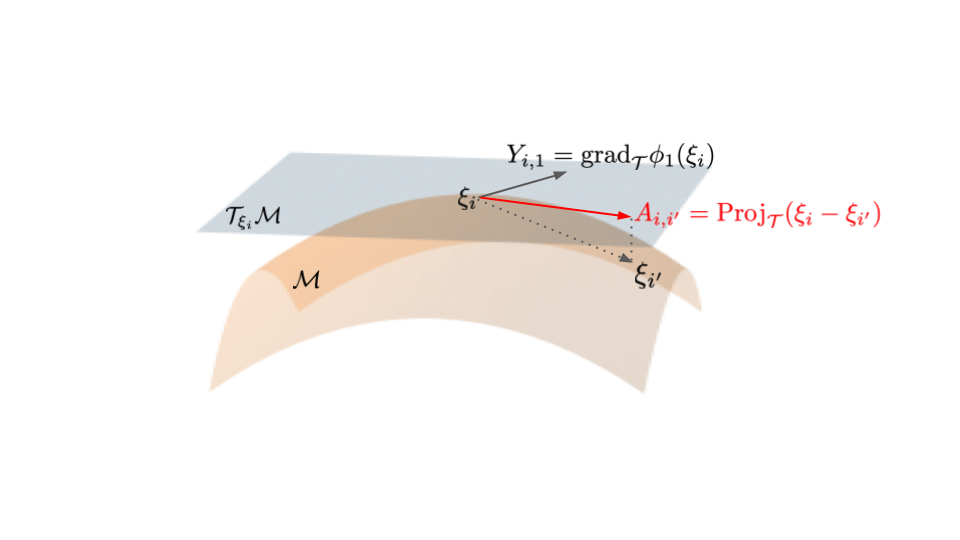
\includegraphics[width=0.48\textwidth]{../Figures/ManifoldSpace3.png}
%&
%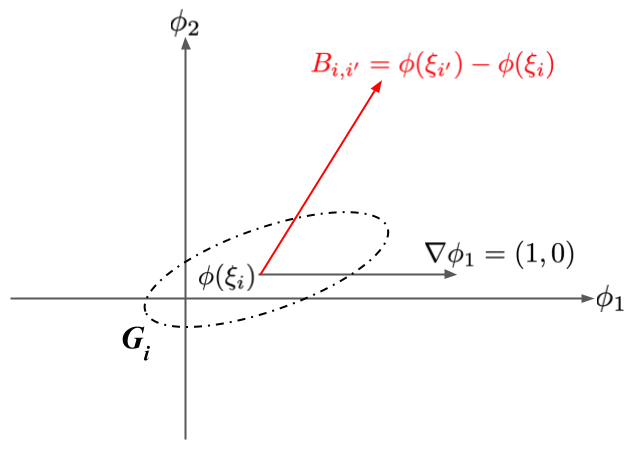
\includegraphics[width=0.48\textwidth]{../Figures/Embedded_space2.png}
%\\
%\end{tabular}
%\caption{\label{fig:pullback} Left: $\M$ with a tangent subspace at $\xi_i$, the projection $A_{i,i'}$ of $\tilde{\xi}_{i'}$ onto $\txim$ (in red), and the manifold gradient $\grad_\M\phi_1(\xi_i)$ of the first embedding coordinate $\phi_1$ (in black). The Riemannian metric on  $\M$ is the identity. Right: for $m=d=2$, $\phi(\M)$ is a (subset of) $\rrr^2$. The dotted ellipse around $\phi(\xi_i)$ represents the push-forward Riemannian metric $G_i$; in red is shown $B_{i,i'}=\phi(\xi_{i'})-\phi(\xi_i)$;  $A_{i,i'}$ is the (approximate) mapping of $B_{i,i'}$ through $D\phi^{-1}(\xi_i)$ (as in \eqref{eq:rmetric0}). The gradient $\grad_{\phi(\M)}\phi_1=\nabla \phi_1$ is trivially the first unit vector (in black). Because $(\M, \id)$ is isometric with $(\phi(\M),\g)$, the unknown $Y_{i,1}=\grad_{\txim}\phi_1$ can be obtained  from the known $A_i,B_i$ and the unit vector by solving a linear system, as in equation \eqref{eq:yi-manifold2}.}
%\end{figure}



\subsection{The \flassoalg~formulation}
\label{sec:flasso-manifold}
Recalling our assumption that $\phi=h\circ g_S$, we shall denote by
$h_k$ the $k$-th component of the vector valued function $h$.
  Recall that $X_i$ defined in
\eqref{eq:X-manifold} contains the gradients of the dictionary
functions $g_j$, and that  $y_{ik}\in \rrr^d$, the $k$-th column of $Y_i$, represents the coordinates of $\grad_{\M}\phi_k(\xi_i)$ in the chosen basis of \txim.
Further, let
%
\beq \label{eq:beta-ijk} \beta_{ijk}=\fracpartial{h_k}{g_j}( g_j( \xi_i)),
\quad \beta=[\beta_{ijk}]_{i,k,j=1}^{n,m,p}, \eeq
\beq \label{eq:betas-manifold}
\beta_j=\operatorname{vec}(\beta_{ijk},\;i=1:n,k=1:m)\in\rrr^{mn},
\quad \beta_{ik}=\operatorname{vec}(\beta_{ijk},\;j=1:p)\in\rrr^{p}.
\eeq
%
In a regression of $Y_{1:n}$ on $X_{1:n}$, $\beta_{ik}$ is the set of regression
coefficients of $y_{ik}$ onto $X_i$. Further, $\beta_j$ represents
the vector of regression coefficients corresponding to the effect of
function $g_j$, which form {\em group} $j$ in the {\em Group Lasso} \citep{Yuan2006-af}
problem defined below. The size of each group is $mn$.

We minimize the  the following objective function w.r.t. $\beta$.
%
\beq\label{eq:flasso-manifold}
J_{\lambda}(\beta)\;=\;\frac{1}{2}\sum_{i=1}^n\sum_{k=1}^m||y_{ik}-X_i\beta_{ik}||^2+\frac{\lambda}{\sqrt{mn}}\sum_{j=1}^p||\beta_j||.
\eeq
%
This is a convex optimization problem, known as the Group Lasso, introduced by \citet{Yuan2006-af}. 
The first term of the objective is the least squares loss of
regressing $Y_{1:n}$ onto $X_{1:n}$. The second is a regularization
term, which penalizes each group $\beta_j$ by its Euclidean
norm. Note that $||\beta_j||$ encourages most $\beta_j$ groups to be
identically 0. The normalization of the regularization coefficient
$\lambda$ by the group size $mn$ follows \citet{Yuan2006-af}. 

The use of Group Lasso for sparse functional regression was introduced in \citet{MKoelleZhang:arxiv1811-11891}, where recovery conditions for the objective function \eqref{eq:flasso-manifold} are given.

Note that $J_\lambda(\beta)$ is invariant to the change of basis
$T_i$. Let $\tilde{T}_i=T_i\Gamma$ be a different basis, with
$\Gamma\in \rrr^{d\times d}$ a unitary matrix. Then,
$\tilde{y}_{ik}=\Gamma^Ty_{ik}$, $\tilde{X}_i=\Gamma^TX_i$, and
$||\tilde{y}_{ik}-\tilde{X}_i\beta||^2=||y_{ik}-X_i\beta||^2$.

\subsection{Computation, normalization, and tuning}
\paragraph{Computation}
\label{sec:ouralg-computation}
The first two steps of \ouralg~are construction of the neighborhood
graph and estimation of the Laplacian $L$. As shown in Section
\ref{sec:background}, $L$ is a sparse matrix, hence \rmalg~can be run
efficiently by only passing values corresponding to one neighborhood
at a time. Note that in our examples and experiments, Diffusion Maps
is our chosen embedding algorithm, so the neighborhoods and Laplacian are already available, though in general this is not the case.

The second part of the algorithm estimates the gradients and
constructs matrices $Y_{1:n},X_{1:n}$.  The gradient estimation
runtime is $O(qd^2 + nd^3)$ where $q$ is the number of edges in the
neighborhood graph, using Cholesky decomposition-based
solvers. Finally, the last step is a call to the \glassoalg, which
estimates the support $S$ of $\phi$. The computation time of each
iteration in \glassoalg~is $O(n^2 m^2 pd)$.  For large data sets, one
can perform the ``for'' loop over a subset $\I\subset[n]$ of the
original data while retaining the geometric information from the full
data set. This replaces the $n$ in the computation time with the
smaller factor $|\I|$.

\paragraph{Normalization}
\label{sec:ouralg-normalization}
Multiplying $g_j$ by a non-zero constant and dividing
its corresponding $\beta_j$ by the same constant leaves the
reconstruction error of all $y$'s invariant, but affects the norm
$||\beta_j||$. Therefore, the relative scaling of the dictionary
functions $g_j$ can influence the recovered support $S$, by favoring
the dictionary functions whose columns have larger norm.

We therefore follow \citet{Haufe2009-yt} in normalizing all columns of the regression matrix to 1. When the dictionary functions $g_j$ are defined on $\M$, but not
outside $\M$, we calculate the {\em normalizing constant}
\beq \label{eq:gammaj-discrete-M}
\gamma_j^2\;=\;\frac{1}{n}\sum_{i=1}^n\|\grad_{T_i} g_j(\xi_i)||^2;
\eeq
%
then we set $g_j\leftarrow g_j/\gamma_j$.  The above $\gamma_j$ is the
finite sample version of $\|\grad_\T g_j\|_{L_2(\M)}$, integrated
w.r.t. the data density on $\M$.

When the dictionary functions are defined on a neighborhood around $\M$ in $\rrr^D$, we compute the normalizing constant with respect to  $\nabla_\xi g_j$. That is,
\beq \label{eq:gammaj-discrete-xi}
\gamma_j^2\;=\;\frac{1}{n}\sum_{i=1}^n\| \nabla_\xi g_j(\xi_i)\|^2.
\eeq
Then, once again, we set $g_j\leftarrow g_j/\gamma_j$. Doing this favors dictionary functions whose gradients are tangent to the manifold $\M$, and penalizes the $g_j$'s which have large gradient components perpindicular to $\M$.

\paragraph{Tuning}
\comment{ 1a sentence on the effect of lambda: large$=$ smaller support,
  etc, 2. for single chart, .... 3. for multiple charts s at least
  d. 4. shall we talk about this or not? in standard lasso cv; we are
  considering it too.  } 
 As the tuning parameter $\lambda$ is
increased, the cardinality of the support decreases.  Tuning
parameters are often selected by cross-validation in Lasso-type
problems, but this is not possible in our unsupervised setting. We
base our choice of $\lambda$ on matching the cardinality of the
support to $d$. In Section 
\ref{sec:theory}, we give sufficient conditions for when $s=d$.

\comment{
However, one can also accept $s>d$
when functions are coherent, like when a dihedral angle has multiple
equivalent formulations, or when no single dictionary function can
parametrize the manifold, like when $\phi$ has piecewise functional
support. A recursive procedure, in which functions discovered to be in
the support are removed from the dictionary and the algorithm is rerun
to uncover dependencies on remaining functions, could also be
used.
}

\comment{In manifolds which cannot be represented by a single chart, the
situation is more complicated, depending on the topology of the
co-domains of the functions $g_j$, and also the quality of the dictionary. For example, in the toluene data
presented in Section \ref{sec:exps}, the manifold is a
circle. This cannot be covered by a single chart, but it can be
parametrized by a single function in the dictionary, the angle of the
bond torsion in Figure \ref{fig:mds-toluene} since the discontinuity of the dictionary function is only at a point of measure zero; hence $s=d$.  The case $s>d$ occurs
when no single dictionary function can parametrize the manifold. For example, when $\M$ is a circle in the plane $(\xi_1,\xi_2)$ and the dictionary consists of the coordinate functions, i.e. $\G=\{g_1\equiv \xi_1,g_2\equiv \xi_2\}$, neither dictionary function can explain $\M$ globally.  Furthermore, when
$\G$ is not a functionally independent set, it is possible that the
parametrization of $\M$ by $\G$ is not unique. In this case, the minimizer of $J_\lambda$ in equation \eqref{eq:flasso-manifold} will be one of the possible support sets $S$.}

\subsection{Variants and extensions}
The approach utilized here can be extended in several interesting
ways. First, our current approach explains the embedding coordinates
$\phi$ produced by a particular embedding algorithm. However, the same
approach can be used to directly explain the tangent subspace of $\M$,
independently of any embedding.

Second, one could set up \flassoalg~problems that explain a single
coordinate function.  In general, manifold coordinates do not have
individual meaning, so it will not always be possible to find a good
explanation for a single $\phi_k$.  However, Figure \ref{fig:mds-ethanol} shows
that for the ethanol molecule, whose manifold is a torus, there exists
a canonical system of coordinates in which each coordinate is
explained by one torsion.

Third, in future work, we plan to examine more closely cases such as the above. It is known \citep{AbrahamMarsden} that Hamiltonian systems are associated with tori; hence, it is natural to consider dictionaries of functions $g:\M\rightarrow S^1$.

\comment{\mmp{what is this?}Fourth, the pushforward metric associated with each of
the individual functional covariates can be estimated with respect to
the data. This enables estimation of sparse functional support that is
more robust to curvature than our current approach, , where the
codomain of $g_j$ is assumed to have identity metric, and is analogous
to finding a flat parameterization of $\M$. Normalization is
equivalent to saying that the metric on the codomain of the dictionary
functions is unknown by a constant factor, while the definition of
norm we use assumes that the metric on the codomain cancels out the
metric on $\phi(\M)$.}  \mmp{don't comment with \%. When no more
  needed, just delete. We have all the previous version if we want
  them.  and regularization here?// project or don't project
  gradients?// Step Embedding can be substituted with any other
  embedding algorithm. To lift $Y_i$ in $\rrr^D$, set $Y_i\leftarrow
  T_iY_i$.  }



\section{Related work}
\label{sec:related}
\comment{To our knowledge, ours is the first solution to estimating a function $f$ as a {\em non-linear} sparse combination of functions in a dictionary. Below we cite some of the closest related work.}

With respect to parametrizing manifolds, the early work of
\citet{saulRoweis:03jmlr} and \citet{tehRoweis:nips} (and references therein)
proposes parametrizing the manifold by finite mixtures of local linear
models, aligned so as to provides global coordinates, in a way
reminiscent of LTSA \citep{ZhangZ:04}. \mmp{also parametrization from paper by
  chris fu}

{\em Gradient Learning} \citep{Ye2012} recovers non-zero partial
derivatives via Group Lasso type regression as methods of variable
selection and dimension reduction. Their work does not rely on a functional dictionary like ours as input,
is concerned with estimating the gradient of a single regression function,
and is in a supervised setting.

The {\em Active Subspace} method of \citet{Constantine2014} uses the information in the gradient to discover a subspace of maximum variation of a function $f$. This subspace is given by the principal subspace of the matrix $C=E_\rho[\nabla f\nabla f^T]$, where $\rho $ is a weighting function averaging over a finite or infinite set of points in the domain of $f$. While this method uses the gradient information, it can only find a global subspace, which would not be adequate for function composition, or for functions defined on non-linear manifolds.

The work of \citet{Brunton-2016dt} is similar to ours in that it uses a
dictionary and the idea of differential composition. The goal is to identify the functional equations of
non-linear dynamical systems by regressing the time derivatives of the
state variables on a subset of functions in the dictionary, with a
sparsity inducing penalty. The recovered functional equation is {\em
  linear} in the dictionary functions, hence any non-linearity in the state variables must be explicitly included in the dictionary. On the other hand, when the functional equation can be expressed as a sum of dictionary functions, then the system is completely identified.

A point of view different from ours is that a set of $d$ eigenvectors of
the Laplace-Beltrami operator $\Delta_{\M}$ are a parametrization of
$\M$. Hence, the Diffusion Maps coordinates could be considered such a
parametrization \citep{coifman:06,CoiLafLeeMag05,Gear2012-rj}. \mmp{it is not known how many needed; but we also don't know about our method.} In
\citet{mohammedNarayanan:localpcs17}, it was shown that principal curves
and surfaces can provide an approximate manifold parametrization. Our
work differs from these in two ways: (1) first, the
explanations we obtain are endowed with the physical meaning of the
domain specific dictionaries, (2) less obviously, descriptors like
principal curves or Laplacian eigenfunctions are generally still
non-parametric (i.e exist in infinite dimensional function spaces),
while the parameterizations by dictionaries we obtain (e.g the
torsions) are in finite dimensional spaces. \citet{Dsilva2018-dz} tackles the
related problem of choosing among the infinitely many Laplacian
eigenfunctions $d$ which provide a $d$-dimensional parametrization of
the manifold; the approach is to solve a set of Local Linear Embedding
\citep{roweis:00} problems, each aiming to represent an eigenfunction
as a combination of the preceding ones. This method reduces the number of "covarying" eigenfunctions but fails to provide physical meaning to the selected functions. 

In \citet{Dsilva13-Nonlinear} the authors consider finding nonlinear intrinsic variables of an observed stochastic process. Suppose that $Y(t)=f(x(t))$ where $t$ is a time parameter, $Y(t)$ is the observed process, and $x(t)$ is a unknown $d-$dimensional stochastic processes driven by stochastic differential equations. The authors further assume that $f$ is bi-Lipschitz so that they can approximate the Euclidean distance in $x$ space by Mahalanobis distance in $Y$ space.  By plugging in this distance into the Gaussian RBF kernel they use the diffusion map to find the function $x$. In this setting, the dictionary functions are unknown. But the parametrization is defined if the manifold and the dictionary functions only differs from a bi-Lipschitz mapping.

Pulling back the gradients from an embedding of the data to $\T_{\xi_i}\M$ by solving a least squares problem was used in \citet{Luo2009-mp}. There, the pull-back was from an approximately isometric mapping of the original data. Hence, the Riemannian metric was not considered. 

\mmp{Autoencoders learn parametric embeddings of fixed $m$; \mmp{shall we compare}. However, there is no a-priori guarantee that the learned function is a manifold outside the data points. \mmp{This would be a problem for us too; except that we know the functions in $\G$ so we can presumably check. }}


\section{Theoretical results}
\label{sec:theory}

Here we study the conditions under which $f=h\circ g_S$ can be represented over a dictionary $\G$ that contains $g_S$. Not
surprisingly, we will show that these are \emph{functional independency}
conditions of the dictionary.

\subsection{Functional dependency}
\label{sec:existence}

We first study when a set of functions on an open subset
$U\subset\mathbb{R}^d$ can be \emph{almost smoothly} represented with a subset of
functionally independent functions. The following lemma implies that
if a set of non-full-rank smooth functions has a constant rank in a
neighborhood, then locally we can choose a
subset of these functions such that the other functions can be smoothly
represented by them. This is a direct result from the constant rank
theorem.

\begin{lemma}[Remark 2 after \cite{Zorich} Theorem 2 in Section 8.6.2]
Let $f:U\rightarrow \rrr^m$ be a mapping defined in an neighborhood
$U\subset \rrr^d$ of a point $x\in \rrr^d$. Suppose $f\in C^\ell$, the rank
of the mapping $f$ is $k$ at every point in $U$, and
$k<m$. Moreover, assume that the principal minor of order $k$ of the
matrix $Df$ is not zero at $x$. Then in some neighborhood of $x\in U$ there
exist $m-k \ C^\ell$ functions $g_i,i=k+1,\cdots,m$ such that
\begin{equation}
 	f_i(x_1,x_2,\cdots,x_d) = g_i(f_1(x_1,x_2,\cdots,x_d),f_2(x_1,x_2,\cdots,x_d),\cdots,f_k(x_1,x_2,\cdots,x_d)).
 \end{equation} 
 \label{lem:representation}
\end{lemma}

Applying this lemma we can construct a local representation of a
subset in $g_S$. The following classical result in differential
geometry enables us to expand the above lemma from local to global.

We start with the definition. A {\em smooth partition of unity subordinate to $\{U_\alpha\}$} is an indexed family $(\psi_\alpha)_{\alpha\in A}$ of smooth functions $\psi_\alpha:\mathcal{M}\rightarrow \rrr$ with the following properties:
\begin{enumerate}[(i)]
	\item $0\leq \psi_\alpha(\xi)$ for all $\alpha \in A$ and all $\xi\in \mathcal{M}$;
	\item supp $\psi_\alpha \subset U_\alpha$ for each $\alpha\in A$;
	\item Every $\xi\in\M$ has a neighborhood that intersects supp $\psi_\alpha$ for only finitely many values of $\alpha$;
	\item $\sum_{\alpha \in A}\psi_{\alpha}(\xi)=1$ for all $\xi\in \M$.
\end{enumerate}


\begin{lemma}[\cite{smoothmfd} Theorem 2.23]
Suppose that $\M$ is a smooth manifold, and $\{U_\alpha\}_{\alpha\in A}$ is any indexed open cover of $\M$. Then there exists a {smooth} partition of unity subordinate to $\{U_\alpha\}$.
\label{lem:partition}
\end{lemma}

Now we state our main results.
\begin{theorem}\label{thm:uni} Assume $\mathcal{G}=\{g_i\}_{i=1}^p$ is the dictionary where $g_{1:p}$ are $C^\ell$ functions in an open set $U \subset \mathbb{R}^d$. For a subset $S\subset[p]$, the notation $g_S$ is a collection of functions in $\mathcal{G}$.  Then let $S'\subset [p],S'\neq S,|S'| < d$ be another subset of $C^\ell$ functions that are full rank at a point.  Suppose that $\ell\geq d+1$. Then there exists a function $\tau:\rrr^{|S'|}\rightarrow \rrr^{|S|}$ that is almost everywhere $C^\ell$ on the range of $g_{S'}$, w.r.t. Lebesgue measure on $\rrr^{|S'|}$, such that $g_S = \tau \circ g_{S'}$ if
\begin{equation} \label{eq:rank}
	\rank\begin{pmatrix} D{g_S} \\ D{g_{S'}} \end{pmatrix} = \rank D{g_{S'}} \ \text{on} \ U
\end{equation}
holds globally. If  $\tau$ is smooth everywhere on the range of $g_{S'}$, then $\eqref{eq:rank}$ holds globally.
\end{theorem}
{\bf Proof} 
First, we show the existence of $\tau$.
Consider $U=U_1\cup U_2$, where $U_1:=\{x: \rank Dg_{S'} = |S'|\}$, and $U_2 = U-U_1$.  $U_1$ is not empty by the assumption. Note that we can select an $|S'|\times |S'|$ submatrix $A_{S',\xi}$ in $Dg_{S'}$ and $\det A_{S',\xi}$ is a continuous function (and thus nonzero) in a neighborhood. This shows that $U_1$ is a nonempty open set. Locally, $g_{S'}$ is a diffeomorphism to its image; therefore $g_{S'}(U_1)$ contains an interior point, and thus has positive measure in $\rrr^{|S'|}$. From Sard's theorem \citep{smoothmfd}, we know that the range of $g_{S'}(U_2)$ is of Lebesgue measure zero in $\rrr^{|S'|}$. Therefore it suffices to show that there exists a $\tau\in C^\ell$ on $g(U_1)$, and we can define arbitrary value for $\tau$ on $g(U_2)$. To simplify the notation we use $U$ to denote $U_1$ in the following proof. By definition of $U_1$, we know that $g_{S'}$ is a diffeomorphism between $U$ and $g_{S'}(U)$. So the inverse $g_{S'}^{-1}$ is well defined and $C^\ell$. Also denote $s=|S|$ and $s'=|S'|$.
Let
\begin{equation}
	g_{S'\sqcup S}(\xi) = \begin{pmatrix}g_{S'}(\xi)\\g_{S}(\xi)\end{pmatrix},
\end{equation}
and use $D{g_{S'\sqcup S}}$ to denote the l.h.s. matrix in \eqref{eq:rank}. Here $\sqcup$ means disjoint union. To be specific, we use $g_{j_i}$ to denote the $i-$th function in the collection $[g_{S'};g_S]$
When the rank of $Dg_{S\sqcup S'}$ equals the rank of $D_{g_{S'}}$,
Lemma \ref{lem:representation} implies that there exists some
neighborhood $U_x\in\rrr^d$ of $x$ and $C^\ell$ functions
$\tau_x^i:\rrr^{|S'|}\rightarrow \rrr,i=s'+1,s'+2,\cdots,s'+s$ such that
\begin{equation}
	g_{j_i}(\xi) = \tau_x^i(g_{j_1}(\xi),\cdots,g_{j_{s'}}(\xi)),\ \text{for} \ i=s'+1,s'+2,\cdots,s'+s, \ \xi\in U_x.
\end{equation}
Here we should notice that $\tau_x^i$ is defined only on $g_S(U_x)$. Since this holds for every $x\in U$, we can find an open cover $\{U_x\}$ of the original open set $U$. Since each open set in $\rrr^d$ is a manifold, the result of partition of unity in Lemma \ref{lem:partition} holds, namely that $U$ admits a smooth partition of unity subordinate to the cover $\{U_x\}$. We denote this partition of unity by $\psi_x(\cdot)$.
\par
Hence we can define 
\begin{equation}
\tau^i(y) = \sum_{x\in U} \psi_x(g_{S'}^{-1}(y))\tau_{x}^i(g_{S'}(y)),\quad y\in g_{S'}(U).
\end{equation}
where $\tau^i$ is a function mapping from $g_{S'}(U)\rightarrow \rrr$.
For each fixed $x \in U$, the function
$y\rightarrow \psi_x(g_{S'}^{-1}(y))\tau_x^i(y)$ for $y\in g_{S'}(U)$ is $C^\ell$.  According to the
properties of partition of unity, in a local neighborhood of each point, this is a summation of finitely many smooth functions.  Then this $\tau^i$ will be a $C^\ell$ function on $g_{S'}(U)$. Also, by $1=\sum_x \psi_x(\xi)$, it holds that $\tau^i(g_{S'}(\xi))=g_{j_i}(\xi)$ for any $i=s'+1,\cdots,s'+s$.
\par Therefore,
globally in $U$ we have
\begin{equation}
	 g_{S\sqcup S'}^i(\xi) = \tau^i(g_{1}(\xi),\cdots,g_{s'}(\xi)),\ \text{for} \ i=s'+1,s'+2,\cdots,s'+s,\ \xi \in U.
\end{equation}
And $g_S(\xi)$ is the concatenation of the last $s$ functions. 

\par Now we prove the reverse implication. If $\rank Dg_{S\sqcup S'}>\rank Dg_{S'}$, then
there is $j\in S$, so that $Dg_j\not\in \rowrange Dg_{S'}$.  Pick
$\xi^0\in U$ such that $Dg_j(\xi^0)\neq 0$; such an $\xi^0$ must exist
because otherwise it will be in $\rowrange Dg_{S'}$. By the theorem's
assumption, $Dg_{S}=D\tau Dg_{S'}$. This implies that $(Dg_S)^T$ is in
$\rowrange (Dg_{S'})^T$ for any $\xi$. But this is impossible at
$\xi^0$. \hfill $\BlackBox$
\par

This theorem essentially gives a condition for the uniqueness of the explanation. If $S$ is the set found by \ouralg, then checking that there is no subset satisfying the rank condition implies that the explanation is unique in the dictionary. We say that a set of functions $g_S$ on a metric space $X$ is \emph{$C^\ell$ (smooth) functionally dependent} at $\xi$ if there is a subset $S'\subset S,S'\neq S$, a function $\tau:\rrr^{|S'|}\rightarrow \rrr^{|S|}$ and a neighborhood $U$ around $\xi$  such that
\begin{enumerate}[(i)]
\item $g_S = \tau \circ g_{S'}$ on $U$;
\item $\tau$ is $C^{\ell}$ (smooth) globally on $g_{S'}(U)\subset\rrr^{|S'|}$;
\item $y-\tau (y_{S'})\not\equiv 0$ on any neighborhood $O(g_S(\xi))\subset \rrr^{|S|}$. Here $y=(y_1,\cdots,y_{|S|})\in \rrr^{|S|},y_{S'}=(y_i)_{i\in S'}\subset \rrr^{|S'|}$.
\end{enumerate}
$S$ is {\em functionally independent} if it is nowhere functionally dependent. Based on Theorem \ref{thm:uni}, we formulate the rank condition below as a necessary and sufficient condition of functional independence.
\begin{corollary}[Functional Independence]
\label{cor:funind}
Suppose $\mathcal{M}$ is a $d-$dimensional smooth manifold and $g_{S}: \mathcal{M}\rightarrow \rrr^d$ are $d \ C^\ell$ functions. Suppose $g_S(\cal M)$ has a positive measure in $\rrr^d$. Then they are functionally independent on $\mathcal{M}$ iff  $\rank Dg_S(\xi)$ is $d$ everywhere on $\mathcal{M}$ except for a closed subset $W\subset\mathcal{M}$ with no interior point.
\end{corollary}
{\bf Proof}
First we show that the rank condition implies functional independence.
Suppose $g_S$ is functionally dependent. Then by definition we have that $g_S = \tau \circ g_{S'}$ on a neighborhood for some $S'$ with $|S'| < |S|=d$. Then on this neighborhood $\rank Dg_S \leq \rank Dg_{S'} \leq d-1$. This contradicts the assumption. On the other hand, suppose $Dg_S$ is functionally independent; then for any $\xi$ there is a $\rank Dg_S \times \rank Dg_S$ non-degenerate submatrix of $Dg_S(\xi)$ whose determinant is non-zero. Therefore, by the smoothness of $g_S$, there exists a neighborhood $V_0$ such that this submatrix of the Jacobian is invertible in this neighborhood. Therefore, for any $\xi' \in V_0$ we have that $\rank Dg_S(\xi') \geq \rank Dg_S(\xi)$.

We therefore start from the case where $\rank Dg_S = d-1$. Select functions that are full rank at this point, and denote them by $g_{S'}$. There is a neighborhood $V_1$ of $\xi$ with $\rank g_{S'}(\xi)=d-1$. If $\rank Dg_S  = d-1$ holds on some neighborhood $V_2$ of $\xi$, then after selecting a chart $(U,\varphi)$ containing $V_1\cap V_0$,  we have that
\begin{equation}
	\rank\begin{pmatrix} D{g_S\circ \varphi^{-1}} \\ D{g_{S'}\circ \varphi^{-1}} \end{pmatrix} = \rank D{g_{S'}\circ\varphi^{-1}}
\end{equation}
holds on $V_2\cap V_1\cap V_0$. Thus, Theorem \ref{thm:uni} implies that $g_S$ cannot be functionally independent (consider a composition with $\varphi$). Therefore, the set $\{x: \rank Dg_S = d-1\}$ has empty interior in $\mathcal{M}$.
Similarly, in every neighborhood $V_{k}$ of any point where $0\leq \rank Dg_S=k < d-1$, there must be a point such that $\rank Dg_S = k+1$. Then in every neighborhood $V_{k+1}\cap V_{k}$ of this new point there must be a point such that $\rank Dg_S = k+2$.  By induction, there must be a point in $V_k$ such that $\rank Dg_S=d$. Therefore we conclude that the set $W=\{\xi:\rank Dg_S \leq d-1\}$ contains no interior point. Also, it is closed because $\{\xi: \rank Dg_S = d\}$ is open.
\hfill $\BlackBox$

\paragraph{Remarks} Before we step further, here we make some remarks on functional independence.
\begin{enumerate}
\item Our definition of functional independence is slightly different from the classical definition in, for example, \cite{Zorich}.\comment{ for the purpose of interpretation of manifold embedding coordinates explanation.} One can show that our definition implies the classical definition.
\item Mathematically, in Corollary \ref{cor:funind}, the condition on $W$ does not mean $W$ is measure zero on the manifold $\mathcal{M}$. However, it is quite common that $W$ is measure zero and in this case the functional independence is also guaranteed. This requirement is not hard to satisfy. For example, in the case of one-dimensional $\M$, it is sufficient that the dictionary contain one {\em Morse function}. By the Morse lemma \cite{morse}, a Morse function's critical points are isolated.  Hence the decomposition is valid almost everywhere. 
\end{enumerate}

With the previous two results, we are ready for Theorem \ref{thm:mfd}, which guarantees the existence of a $d-$function explanation given a good dictionary in the sense of having a functionally independent subset.
%
\begin{theorem}
\label{thm:mfd}
Let $\mathcal{G}$ and $g_S$ be defined as before. $\mathcal{M}$ is a smooth manifold with dimension $d$ embedded in $\rrr^D$. Suppose that $\psi: \mathcal{M}\subset \rrr^D \rightarrow \rrr^m$ is also an embedding of $\mathcal{M}$ and has a decomposition $\psi(\xi) = h\circ g_S(\xi)$ for every $\xi \in \mathcal{M}$ where $h$ is smooth.
If the dictionary $g_S$ contains $d$ functions denoted by $g_{S'}$,  that are smooth functionally independent on $\cal M$, then there exists a $\widetilde{h}$ such that $\psi = \widetilde{h}\circ g_{S'}$ on every $\xi \in \mathcal{M}$. Here, the
function $\widetilde{h}$ is smooth almost everywhere in the range of $g_{S'}$.
\end{theorem}

{\bf Proof}
Consider the set $U=\{x: \rank Dg_{S'}=d\}$. It is an open subset of the manifold $\cal M$ and therefore a smooth manifold. For each point $x\in U$, select a local chart $(V,\varphi)$ such that $V\subset U$. With the same argument in the proof of Corollary \ref{cor:funind}, we know that there exists a smooth functions $\tau_x$ on $V$ such that $g_S = \tau \circ g_{S'}$ holds on V. Also, since $V$ is an open neighborhood, we conclude that the measure of $g_{S'}(U)\geq g_{S'}(V)$ should be strictly positive. Therefore the partition of unity technique used in the proof of Theorem \ref{thm:uni} can show that there exists a function $\tau$ on $U$ that is smooth over $g_{S'}(U)$ such that $g_S = \tau \circ g_{S'}$ holds globally on $U$. We can define $\tau$ on $\mathcal{M}\setminus U$ to be anything, and Sard's theorem implies that $g_{S'}(U)$ would be a measure zero set in $\rrr^d$.  Finally, we just write $\widetilde{h}=h\circ \tau $
\hfill $\BlackBox$

Here we
assume that a subset of functions with rank $d$ almost everywhere
exists. In fact, on a compact $d-$dimension manifold $\mathcal{M}$, any smooth function $f:\mathcal{M}\rightarrow \rrr^d$ must have at least one singular point.  Think of function $f\circ \pi_1$ where $\pi_1$ is the projection onto the first coordinate. It must attains its maximum value at some point. Then at that point the gradient of this function is zero and the Jacobian must have a rank less than $d$. This example shows that sometimes there does not exist a function $f:\mathcal{M}\rightarrow \rrr^d$ with constant rank $d$. Similar results to Theorem \ref{thm:uni} hold {\em almost
everywhere} if the decomposition $f=h\circ g_S$ holds almost
  everywhere on the manifold $\M$, and the dictionary is smooth on
$\mathcal{M}$ except for a closed set of measure zero. With this
weaker assumption, one can, for example, find one function explaining
the whole circle $S^1$ embedded in $\rrr^2$ except one point.
\mmp{We can go on from here nicely to say that if $f:\M\rightarrow O\neq \rrr^d$ then it's possible.}

In a finite sample setting, Theorem \ref{thm:uni} states that $S$ and $S'$ are equivalent explanations for $f$ whenever \eqref{eq:rank} holds on open sets around the sample points. For example, Theorem \ref{thm:uni} does not have to hold globally. Suppose we are given a solution subset $S$. The interpretation of this result is that we hope $\phi = h\circ g_{S}$ holds almost everywhere on the manifold, and $h$ is smooth on the image of $g$ of the data points. As stated before, we can assume the dictionary contains $d$ functions with rank $d$ almost everywhere. An intuitive way to satisfy this assumption when constructing the dictionary is to select functions that are not varying with the same trend. One can also conduct a sanity check of the rank condition after we get a solution subset $S$. If they are always full rank on these finite samples, we still get meaningful results.  For low dimensional settings, i.e. when $s\geq d$, the Theorem implies
that in general there will be many equivalent explanations of $f$ in
$\G$. Assuming no noise, the solution to (\ref{eq:flasso-manifold}) will be the subset
$S$ that minimizes the penalty term
$\frac{\lambda}{\sqrt{mn}}\sum_{j=1}^p\|\beta_j\|$ on the data set. 

Finally, the success of Group Lasso requires stronger assumptions on the dictionary functions. For example, according to \cite{GO2011}, a particular group $S$ will be recovered by Group Lasso methods, if (1) it is close to perpendicular to the linear subspace generated by all other groups (2) Group features in $S$ are close to orthogonal matrix. In our case, if a sparse representation $\phi=h\circ g_S$ is identified from our Group Lasso formulation, the gradients of functions in $S$ should be close to normal to all other functions in the dictionary, and the gradient in $S$ themselves need to be close to orthogonal. Rank conditions and functional independence assumptions only guarantees the existence of a sparse nonlinear representation of the embedding. Only "good" subset of dictionaries can be recovered with guarantee. 

\mmp{sphere in D dimensions, system of spherical coordinates. how does this apply?}
\mmp{In chem paper, we should discuss how many independent bond torsions can exist, if possible. I'm leaving the calculations below as a reminder. 
See also Delaunay triang,  simplicial complex or not? ask Sara?
 for a molecule with $N$ atoms, the number of quadruples of atoms close enough to interact, which is close to $\binom{N}{4}$; for toluene ($N=15$) $p\leq 1365$, for ethanol ($N=9$) $p\leq 126$, and for aspirin ($N=21$), $p\leq 5985$. \mmp{think of decomposable models/treewidth 3/ graphs over edges/ etc to give a condition. Spanning tree sufficient but not necessary. Think of symmetries, same dihedral}}

% this was gradients-nips-proofs.tex

\section{Experiments}
\label{sec:exps}

We demonstrate \ouralg~ on several manifold learning problems.
First, we illustrate its behavior on a high-dimensional variant of the classical Swiss Roll problem, and show that is recovers the correct internal coordinates across a range of manifold learning methods.  Second, we use it to identify explanations of collective coordinates of Molecular Dynamics (MD) simulations of small molecules. We recover explanations in terms of bond torsions and compare our results with ground truth validated by domain experts. This, as well as more background and details on manifold embeddings for MD simulations, can be found in \cite{ChenMcqueenKoelleMChmielaTkatchenko:mlcules-dum19}.
Section \ref{sec:exp_setup} describes the general experimental procedure, while Section \ref{sec:md} describes molecular-dynamics specific adjustments to this protocol.
Sections \ref{sec:swiss}--\ref{sec:malonaldehyde} describe our experimental results. Code to run experiments is available at \url{https://github.com/sjkoelle/manifoldflasso_jmlr}.

%show that \ouralg~ recovers

%the classical Swiss Roll problem and a torus generated from a rigid model of the ethanol molecule, with a dictionary of bond torsions, as in Figure \ref{fig:molecs}.
%Then, we apply \ouralg~to  real data generated by Molecular Dynamics (MD) simulations of small molecules;

%
\begin{table}[h]
\begin{center}
\begin{tabular}{ | l | c | c | c| c| c | c | c  |c| c | c |  }
\hline
Dataset & $n$ & $N_a$ & $D$  & $d$  & $\epsilon_N $&   $m$ & $n'$ & $p$ & $\omega $ \\ \hline
\srdata & 100000 & NA & 49 & 2 & .18  &  2 &  100 & 51 & 5 \\
%\hline
\redata & 10000 & 9 & 50 & 2 & 3.5  &  3 & 100 & 12 & 5\\
\hline %\hline
\ethdata & 50000 & 9 & 50 & 2 & 3.5 & 3 & 100 & 12  & 5\\
%\hline
\maldata & 50000 & 9 & 50 & 2 & 3.5 & 3 & 100 & 10  & 5 \\
%\hline
\toldata & 50000 & 16 & 50 & 1 &  1.9   & 2& 50 & 32 &  5\\
\hline
\end{tabular}
\end{center}
\caption{Summary of experiments. \srdata~ and \redata~ are toy data, while \toldata, \ethdata, and \maldata~ are from quantum molecular dynamics simulations by \citet{chmielaTkaSauceSchuPMull:force-fields17}. The columns list the experimental parameters as follows; $n$ is the sample size for manifold embedding, $N_a$ is the number of atoms in the system, $D$ is the dimension of $\xi$,  $d$ is the intrinsic dimension, $\epsilon_N$ is the kernel bandwidth, $m$ is the embedding dimension, $n'$ is the size of the subsample used for \ouralg, $p$ is the dictionary size, and $\omega$ is the number of independent repetitions of \ouralg. More details are in Section \ref{sec:exp_setup}}
\label{tab:exps}
\end{table}

\subsection{Experimental setup}\label{sec:exp_setup}

For all of the following experiments, the data consists of $n$ data points in $D$ dimensions, as well an embedding $\phi_{1:m} (\dataset)$.  We assume access to the manifold dimension $d$, a parameter $\epsilon_N$ for estimation of distortion induced by the embedding, and $p$ dictionary functions. Except where otherwise specified, $m$ and $\epsilon_M$ are used in the preliminary step of generating embeddings $\phi_{1:m}$ using the Diffusion Maps algorithm as \embedalg. \ouralg~ is applied to a uniformly random subset of size $n' = |\I|$ and this process is repeated $\omega$ number of times. The regularization parameter $\lambda$ ranges from 0 to a value for which only $d$ dictionary functions persist in the regularization path. These functions are the explanation for the manifold coordinates. These parameters are passed to the \lapalg, \tppalg, \rmalg, and \dpullalg~algorithms.  Parameters are summarized in Table \ref{tab:exps}.

\subsection{Molecular dynamics}{\label{sec:md}

\paragraph{Representing molecular configurations}

The understanding of the {\em slow dynamic modes} of molecules and other atomic systems from Molecular Dynamics simulation data is a well-known application of manifold learning algorithms. In such simulations, the positions of atoms within a molecule are sampled as they proceed through time from some initial conditions. Even though the vector of atomic coordinates can take any value, due to interatomic interactions, the relative positions of atoms within the molecule lie near a low-dimensional manifold. A manifold learning method then learns a set of functions that approximate the data manifold \citet{ChenMcqueenKoelleMChmielaTkatchenko:mlcules-dum19}. We utilize \ouralg~ to approximate this learned manifold using functions with physical meaning: bond torsions. This is an example of data-driven discovery of governing laws of non-linear dynamical systems, and is a novel way to understand long time-scale motions of molecules.

Our data are from quantum-simulations from \citet{chmielaTkaSauceSchuPMull:force-fields17}. Raw MD data consists of $X,Y,Z$ coordinates for each of the $N_a$ atoms of the chosen molecule. For a single observation, we denote these by $r_i \in\rrr^{3N_a}$. The first step in our data  analysis pipeline is to featurize the configuration in a way that is invariant to rotation, translation, mirror symmetry, and scaling. In the present experiments, we follow \citet{ChenMcqueenKoelleMChmielaTkatchenko:mlcules-dum19} and represent a molecular configuration as a vector $a_i \in\rrr^{3 {N_a \choose 3}}$ of the angles formed by triplets of atoms. We then perform an SVD on this featurization, and project the data onto the top $D = 50$ singular vectors to remove linear redundancies; we denote the new data points by $\xi_{1:n}$. The \embedalg~and \tppalg~algorithms work directly with $\xi$ in dimension $D$.

%In order to establish the efficacy of \ouralg~ for this type of data,
%This is sufficient for the types of molecules presented here, as explained in \citet{ChenMcqueenKoelleMChmielaTkatchenko:mlcules-dum19}.

\paragraph{Dictionaries for MD data}

For the \redata, \ethdata, \maldata, and \toldata~experiments, the dictionary consists of bond {\em torsions}, also known as dihedral angles. Given an ordered
4-tuple of atoms $ABCD$, the torsion $g_{ABCD}$ is the
angle of the planes defined by the locations of $ABC$ and $BCD$. Note that $g_{ABCD}\equiv g_{DBCA}\equiv g_{DCBA}\equiv g_{ACBD}$. In a molecule, any two
atoms which are not too distant interact; hence the analyzed molecules have more diatomic interactions than those represented in Figure \ref{fig:molecs} and  diagrams \ref{fig:toluene-bonds}-\ref{fig:mda-bonds}, and consequently more bond torsions.
\skcomment{To keep this sentence appropriate, we should extend to colinear bad dictionaries.  To be honest, I think much of this should be moved to the supplement, and the discussion here should be more high level.}
 %The ability to simultaneously analyze many of these so-called improper dihedral angles is a main feature of our approach.
%skcomment{Us defining 'bonds' is unnecessary and is not technically right}
%We call the segments $AB,BC$, etc. {\em bonds}; atoms $A,D$ are called {\em distal}, and atoms $B,C$ are called {\em central}; $g_{ABCD}$ is called the torsion of the $BC$ bond.
Any torsion $g$ is expressible in closed form as functions of the
planar angles feature vector $a$. In particular, a torsion $g_{ABCD}$
is a function of the angles of the triangles $ABC$, $ABD$, $ACD$, and
$BCD$.  We compute the gradients of the torsions by automatic
differentiation \citep{paszke2017automatic}.

We cannot use the obtained gradients directly in \ouralg, since the angular featurization is an overparameterization of the molecular {\em shape space
$\Sigma_3^{N_a}$} \citep{addicoatcollins:2010,Kendall1989-hu} of
dimension $D'=3N_a-7$, and off-manifold gradients are therefore not well-defined.
For
example, whether one chooses to use triangles $ABC$, $ABD$, and $ACD$,
or $ABC$, $ABD$, and $BCD$ to compute $g_{ABCD}$ has no effect on the value of $g_{ABCD}$, but changes the value of the gradient.
We therefore compute the gradients in the tangent bundle of the shape space as it is embedded in the $\xi$ coordinates. Details are given in Appendix \ref{app:shape-space}. It is on these gradients that we perform the normalization as described in Section \ref{sec:ouralg-computation}.

Remaining specifics of our MD data analytics pipeline are in Appendix \ref{app:dictionary-details}.

\subsection{Synthetic data}\label{sec:syndata}

\paragraph {\ouralg~ on \srdata}
\label{sec:swiss}

In the classic Swiss Roll manifold learning problem, data is sampled
from a two dimensional rectangle and rolled up along one of the two axes, and a manifold learning method is used to learn the coordinate functions of the rectangle.  We demonstrate that \ouralg~ is able to attribute these learned coordinate functions to their respective internal coordinates.  To complicate this simple example, we randomly rotate the 3-dimensional Swiss Roll in 49 dimensions, and construct a dictionary $\G$of $g_{1,2}$, the two manifold-specific coordinate functions, as well as $g_{j+2}=\xi_j$, for $j=1,\ldots 49$, the coordinate functions of the feature space.  We then learn the manifold using four techniques: Local Tangent Space Alignment, Diffusion Maps, Isomap, and using the a priori known 'correct' internal coordinates.  We then apply \ouralg, and show that it is robust to the choice of embedding method. Figure \ref{fig:sw1} demonstrates that \ouralg~ correctly recovers the two manifold-specific coordinate functions in each case, and maps them to the correct coordinate function.

%
\begin{figure}[hbt!]
\begin{tabular}{ccc}
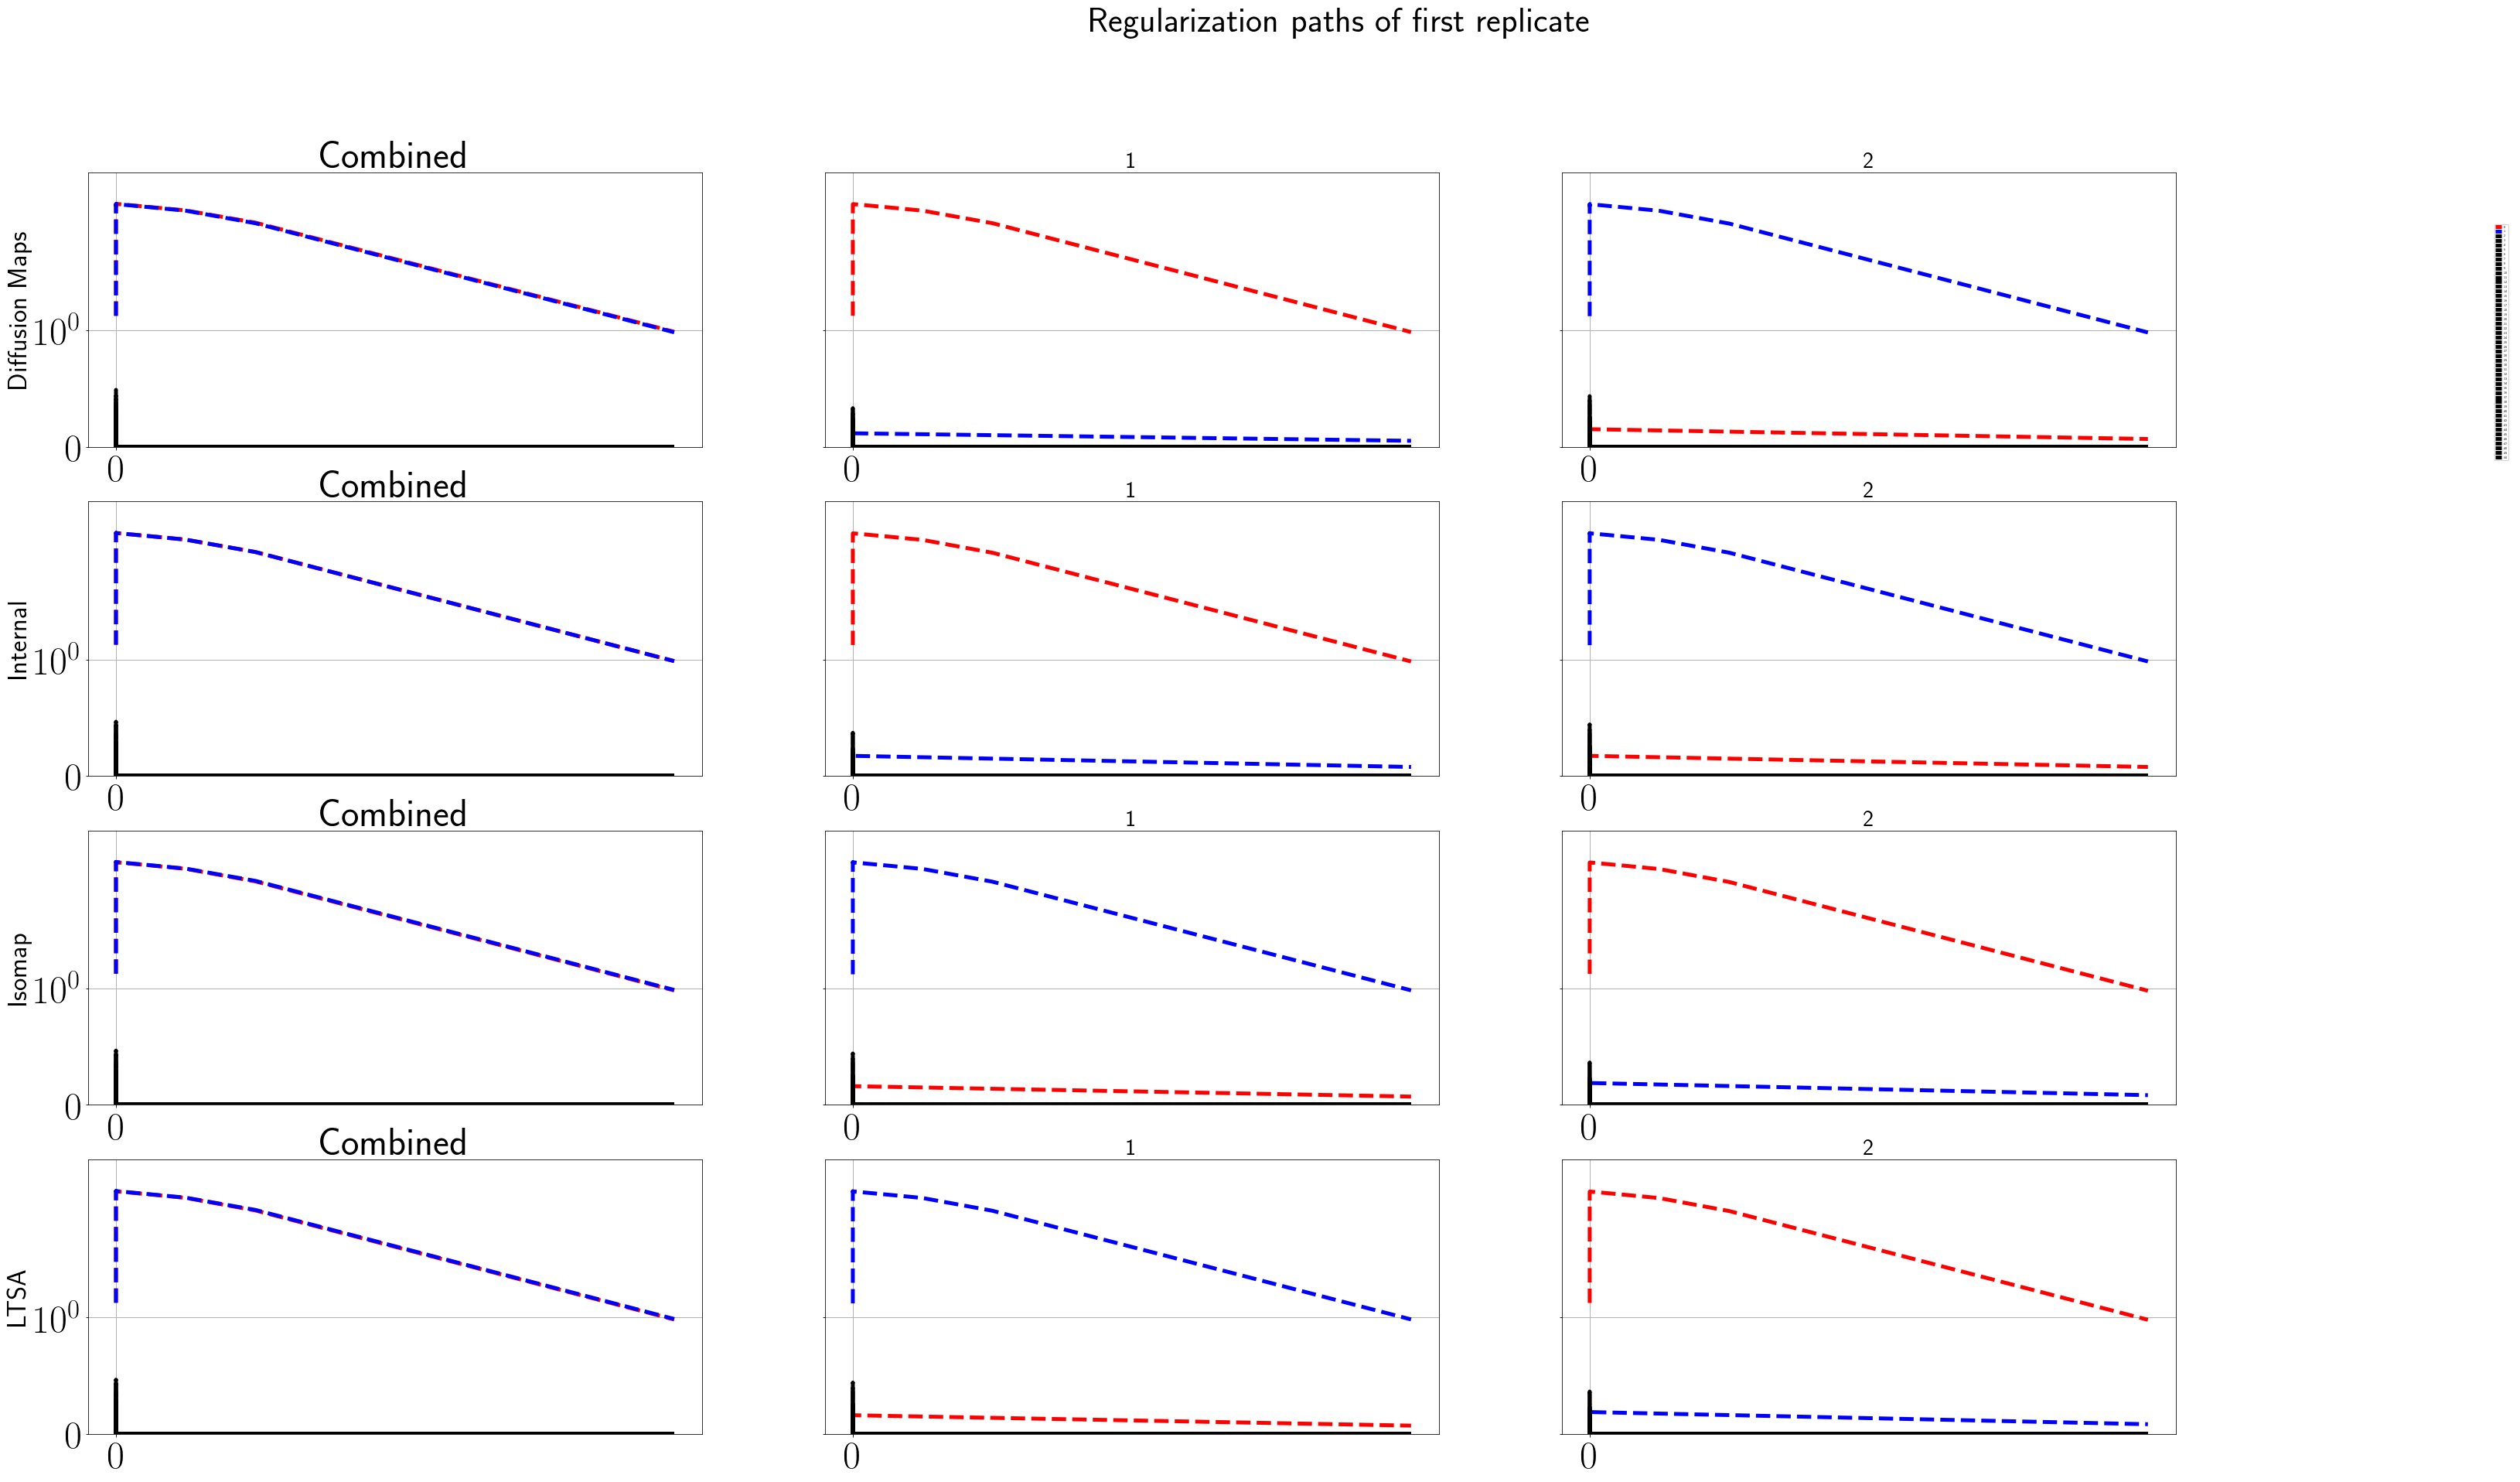
\includegraphics[width = \textwidth]{../Figures/revision_temp/swissroll}
\label{fig:sw} &
&
\end{tabular}
\caption{\skcomment{a) Embeddings of the \srdata dataset.}  b) \srdata~ \ref{fig:sw1} This figure displays the results of one replicate of \ouralg~ for several different embeddings of the \srdata dataset. The left panels displays $||\beta_{1:p}||_2$ as a function of the regularization parameter $\lambda$. The remaining panels display, each for one of the embedding coordinates $\phi_k$, the norm of the vector $\vec(\beta_{i,j,k},\,i=1:n')$ \skcomment{c) Support recovery heatmaps or equivalent.}.
%To be able to include the extreme cases $\lambda=0$ (no regularization) and $\beta_j \equiv 0$ ($j$ excluded from $S$), both figure axes are linear from 0 to 1, and logarithmic for values larger than 1. Error bars summarize the outcomes of the $\omega$ repetitions.
% \ouralg~ selects the internal coordinates over the coordinates of the ambient space for $\lambda \in [1,10]$.
 }
\end{figure}

\paragraph{\ouralg~on a Rigid Ethanol skeleton}\label{sec:rigid}

We demonstrate the efficacy of our method for molecule-type data in a controlled setting by applying it to a simple rigidly-rotating ethanol trajectory.  We first construct an ethanol skeleton composed of the atoms shown in Figure \ref{fig:ethanol-bonds}.  We then sample as we rotate the atoms around the C-C and C-O bonds, giving the simulated trajectory two a priori known degrees of freedom. These two angles are distributed uniformly over grid. This contrasts with the MD-trajectories, which are simulated according to quantum dynamics.
The dictionary (Figure \ref{figtab:eth} in Appendix \ref{app:dictionary-details}) consists of the twelve torsions implicitly defined by the bond diagram. \skcomment{should add spurious torsions. all angles?}.  Figure \ref{fig:ret3} presents the results.  

%, $g_1,g_2$ which correspond respectively to the C-C and C-O bonds marked in Figure \ref{fig:ethanol-bonds}, and two other torsions that by construction do not vary across the manifold.

\comment{Figures \ref{fig:ret1} and \ref{fig:ret2} show the estimated manifold is a two-dimensional surface with a torus topology similar to that observed for the MDS ethanol in Figure \ref{fig:molecs}. As in the MD ethanol, bond torsions $g_1$ and $g_2$ appear to parameterize the manifold. These are the two C-C and C-O torsions which vary by construction in this simulation.}

\ouralg~ identifies pairs of torsions that explain the manifold. These can be visually verified as in Figure \ref{fig:ret1} and \ref{fig:ret2}.  Figure \ref{fig:ret3} shows that, across replicates, \ouralg~ selects pairs of functions with orthogonal gradients out of the colinear functions \skcomment{Overlay selection on cosines?} . Inspecting individual replicates in Figure \ref{fig:ret4}, we can see that these associate particular dictionary elements with particular embedding coordinates that corroborates what we can visually observe in Figure \ref{fig:ret1} and \ref{fig:ret2}, and that the spurious dictionary functions are quickly eliminated.   

%
\begin{figure}[hbt!]
\begin{tabular}{ccc}
\subfloat[$g_1$]{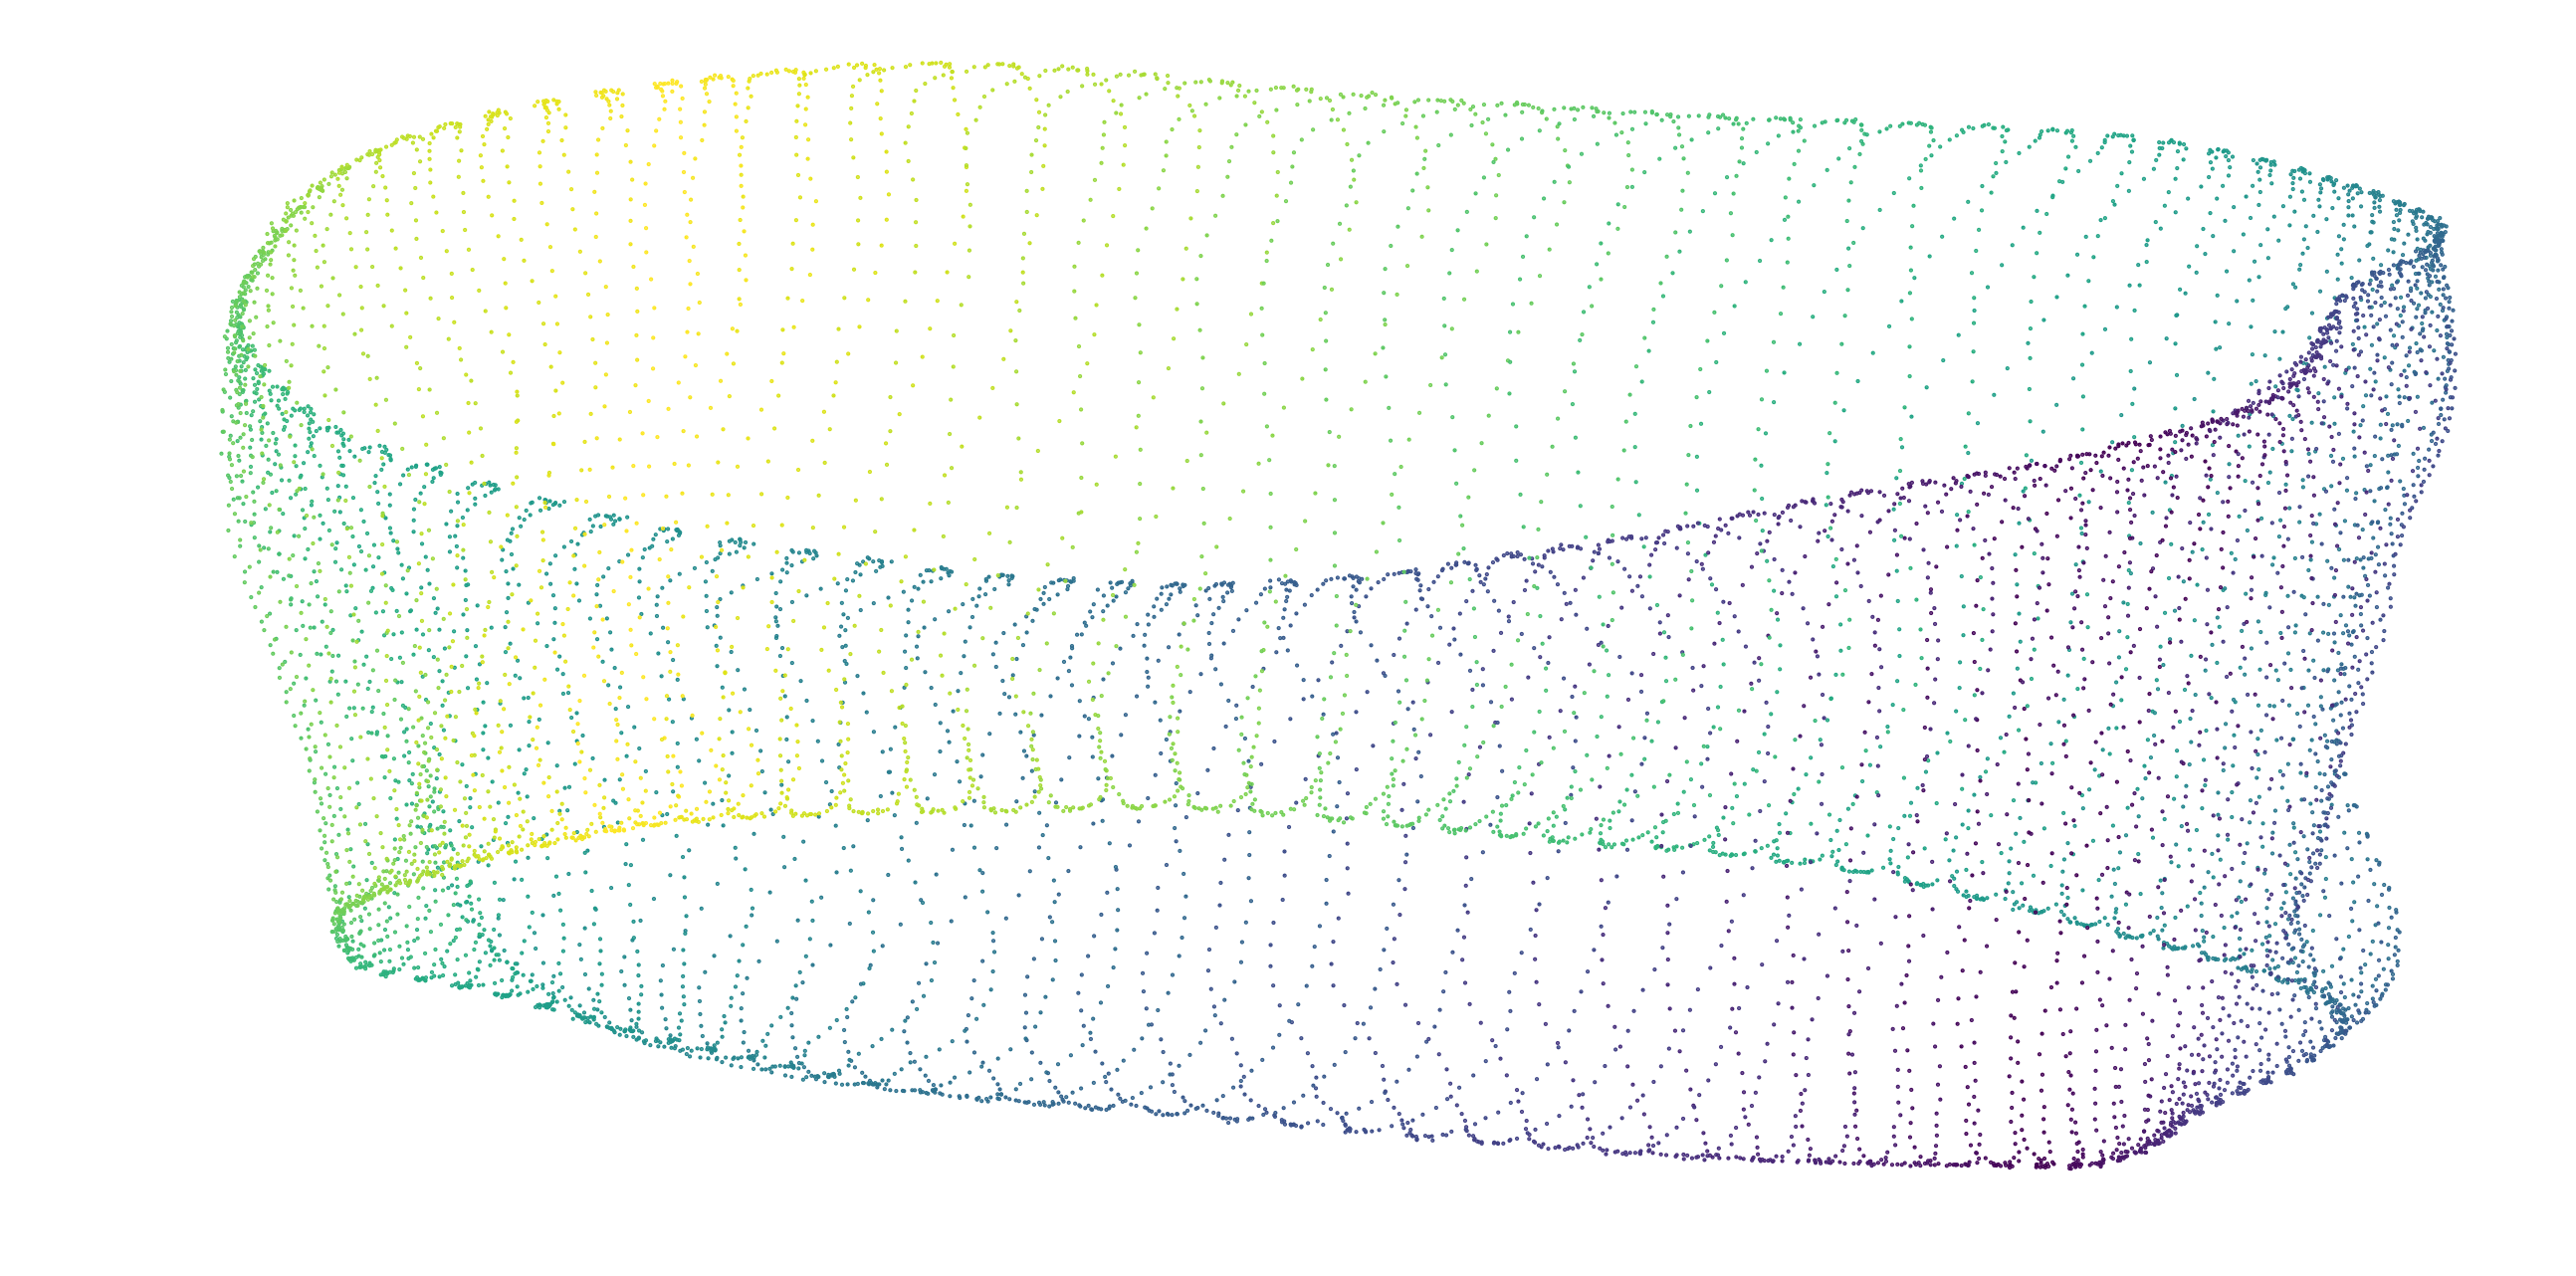
\includegraphics[width = 1in]{../Figures/rigidethanol/April_04_2019_12_51_31/torsion0.png} \label{fig:ret1}}& 
\subfloat[$g_2$]{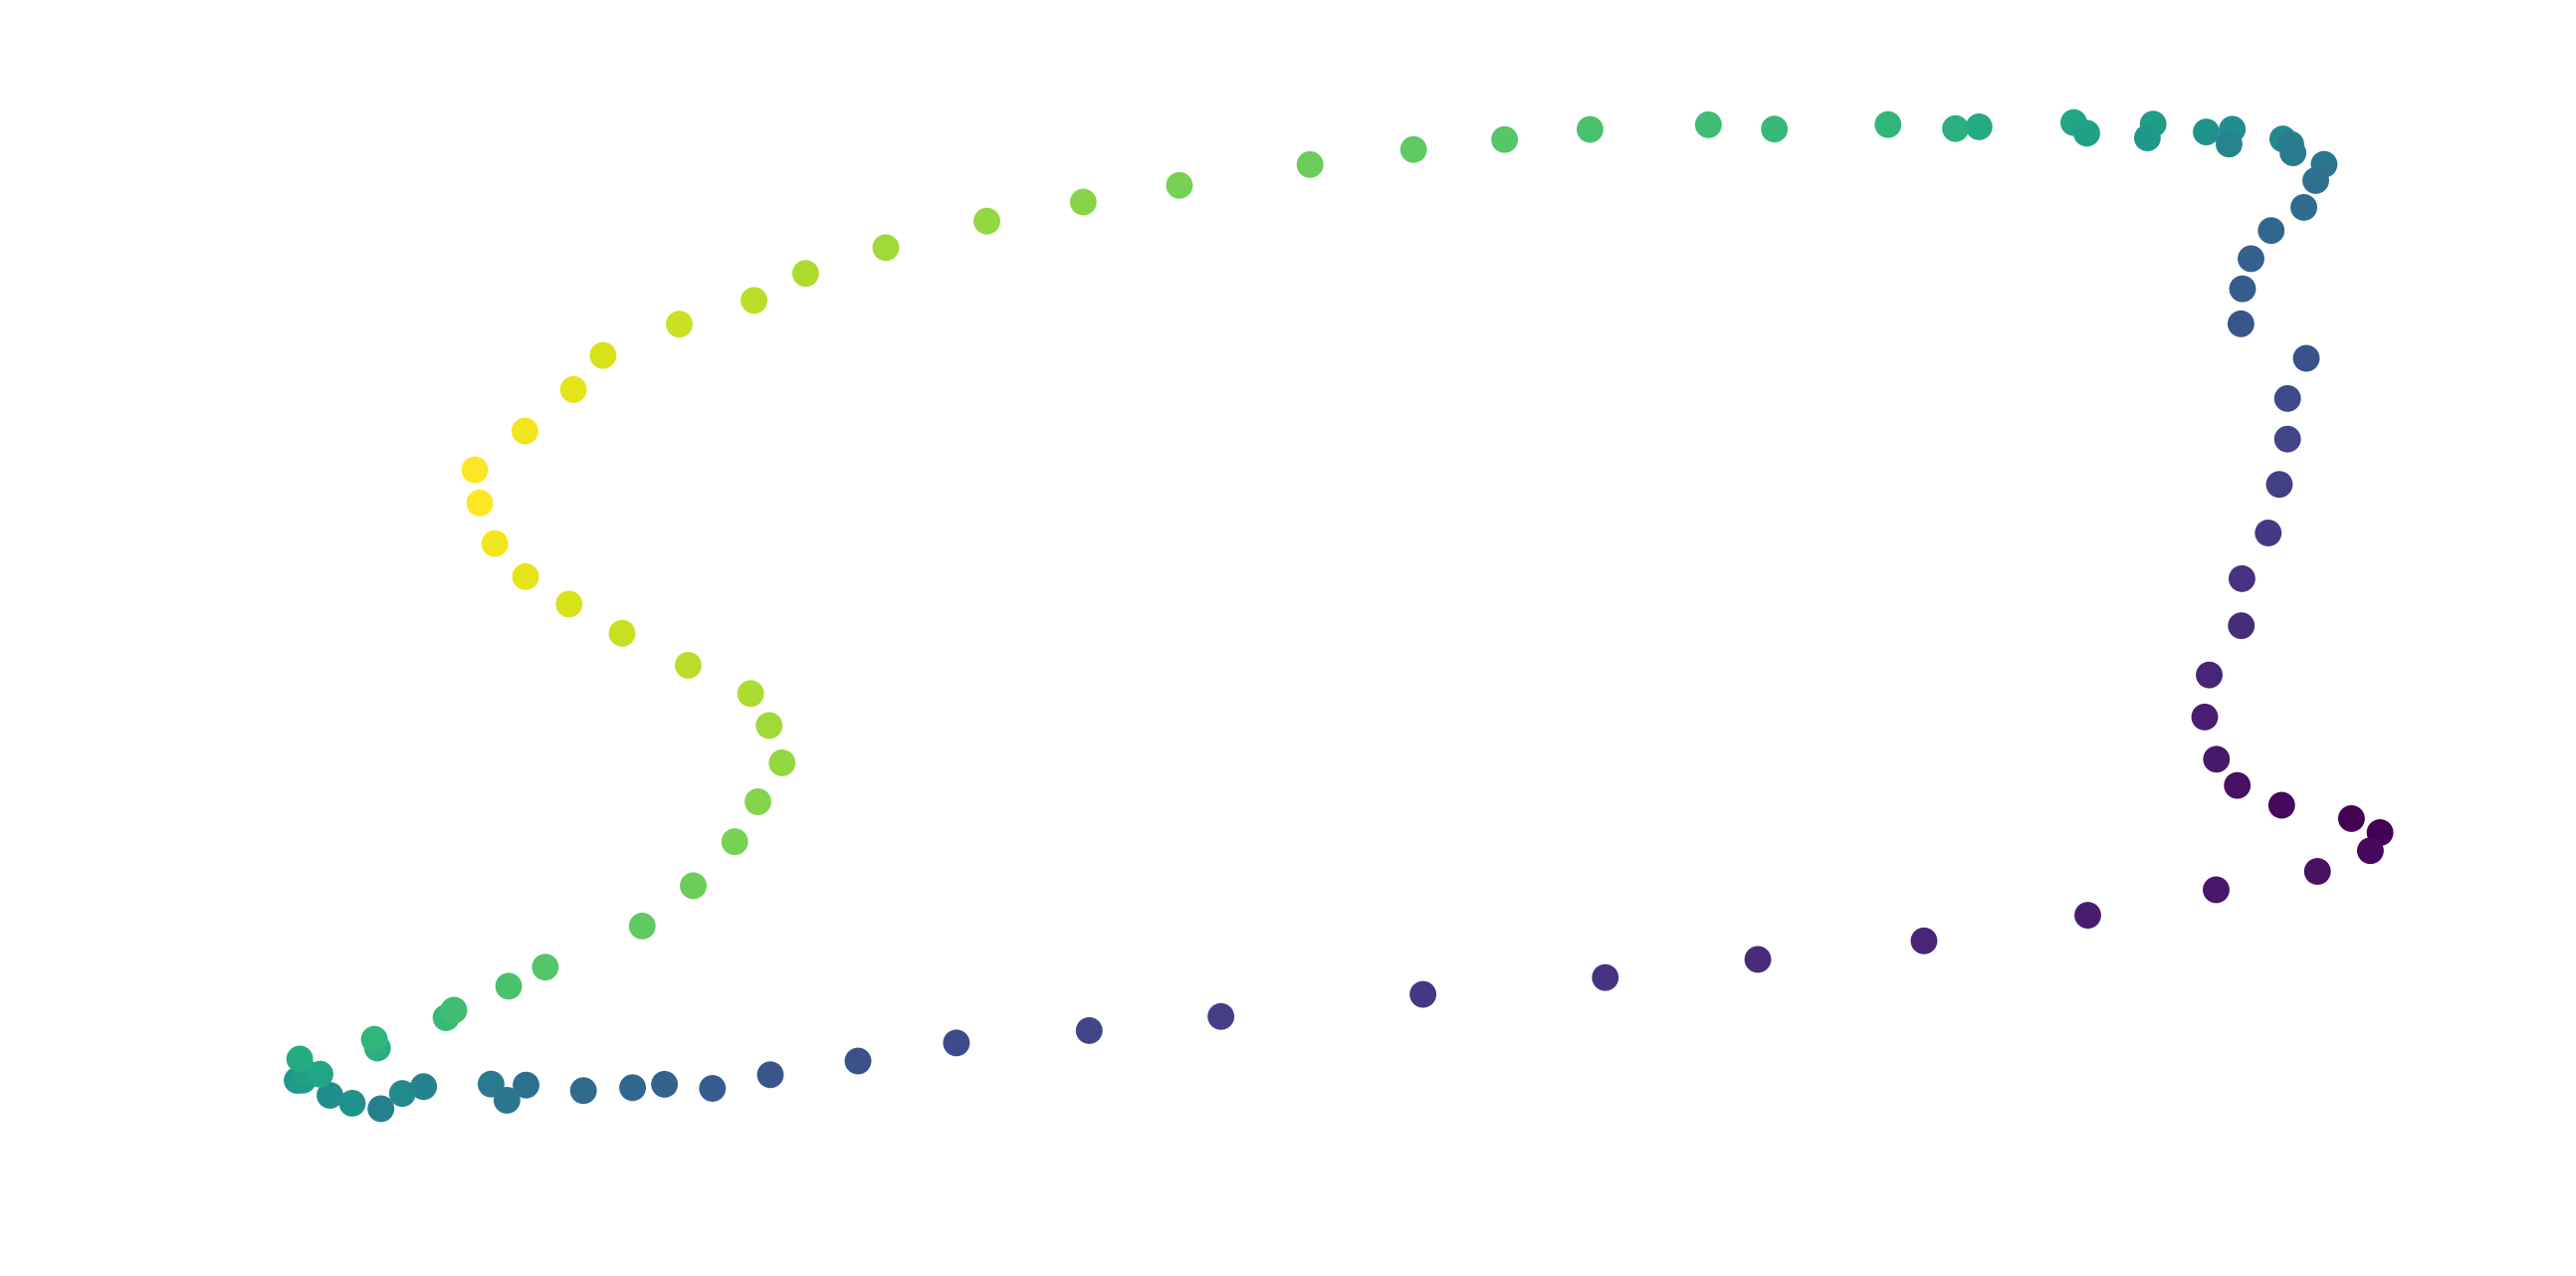
\includegraphics[width = 1in]{../Figures/rigidethanol/April_04_2019_12_51_31/torsion1.png} \label{fig:ret2}} &
 \subfloat[]{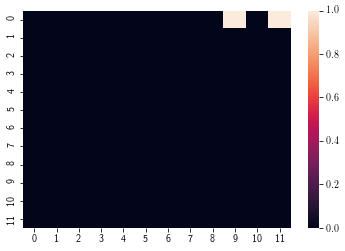
\includegraphics[width = 1in]{../Figures/revision_temp/support_recovery_temp.png} \label{fig:ret3}} \\
 \multicolumn{3}{c}{\subfloat[] {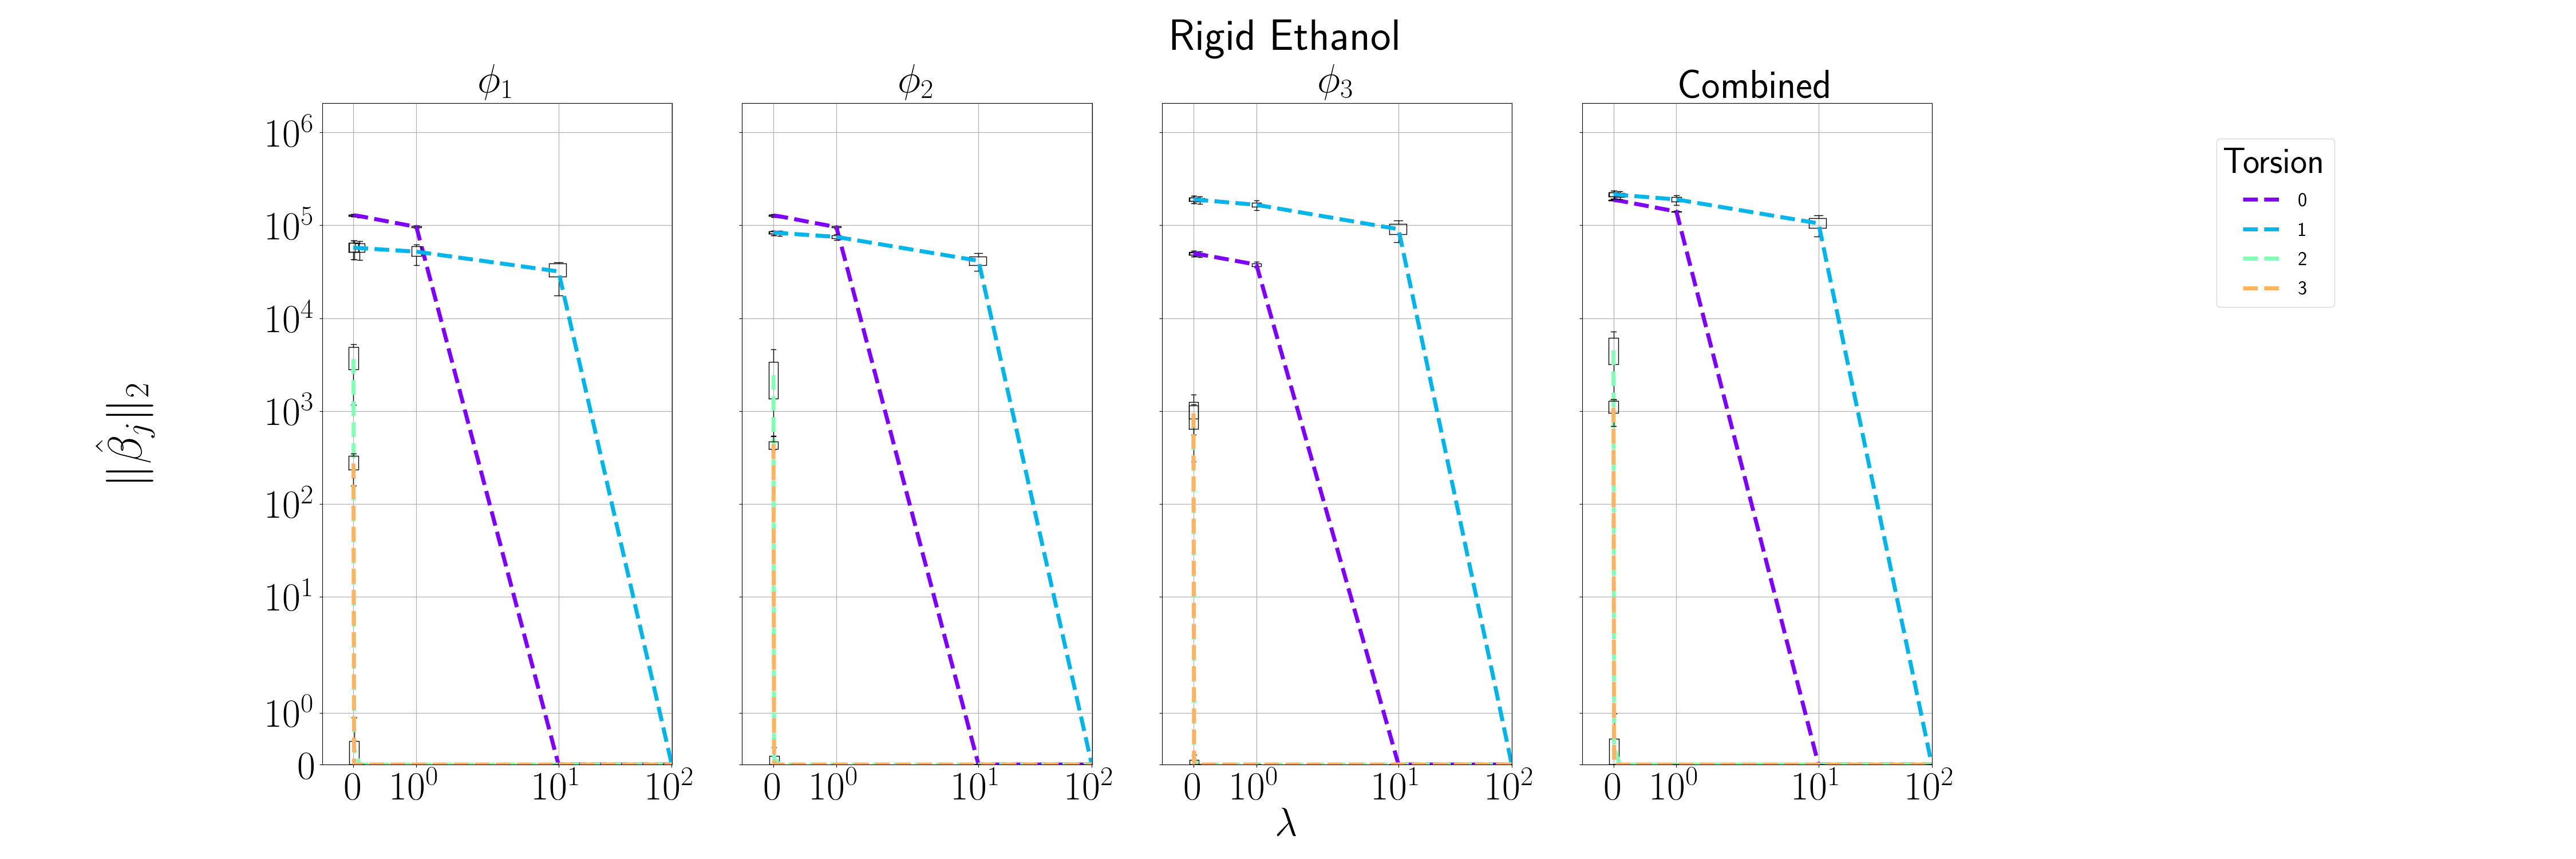
\includegraphics[width = 5in]{../Figures/rigidethanol/April_04_2019_15_15_12/betassymlogbeta_paths_log_n10000nsel100nrepss3rigidcombotoohighiter.png}} \label{fig:ret4}}
%\multicolumn{3}{*}{\subfloat[] 
\end{tabular}
\caption{\redata~ \ref{fig:ret1} The learned manifold colored by the C-C bond torsion $g_1$, the purple bond in Figure \ref{fig:ethanol-bonds}; compare this embedding with the embedding of MD ethanol in Figure \ref{fig:molecs}. \ref{fig:ret2} A radial slice of the embedding colored by the C-O bond torsion $g_2$, the blue bond in Figure \ref{fig:ethanol-bonds}. \ref{fig:ret3} This figure presents the frequency of support recovery across pairs of dictionary elements and replicates. \ref{fig:ret4} Support recovery results for one replicate of \ouralg \skcomment{This is a stand in}. 
%The left panel displays $||\beta_{1:p}||$ as a function of the regularization parameter $\lambda$. The remaining panels display, each for one of the embedding coordinates $\phi_k$, the norm of the vector $\vec(\beta_{i,j,k},\,i=1:n')$. These panels show the relative contribution of each dictionary function to explaining a particular embedding coordinate $\phi_k$. For $\lambda > 1$, $\phi_{1,2}$ are explained by $g_1$, while $\phi_3$ is explained by $g_2$. Axes are linear between $0$ and $1$, and logarithmic above $1$. Error bars summarize the outcomes of the $\omega$ repetitions.
}
\label{fig:rigid-ethanol}
\end{figure}

\subsection{Molecular Dynamics Data}\label{sec:mds_data}

\paragraph{Ethanol}\label{sec:ethanol}

%Ethanol has no p-orbital hybridization, and a more intricate vibrational structure than toluene.
Figure \ref{fig:molecs} shows that the estimated manifold is a two-dimensional toroidal surface, and that the two generators of the torus corresponds to bond torsions $g_1$ and $g_2$.  Our dictionary consists of these two torsions, as well as two other dihedral angles. \ouralg~ identifies that $g_1$ and $g_2$ explain the manifold. Furthermore, it associates $g_1$ with embedding coordinates $\phi_1$ and $\phi_2$ and $g_2$ with $\phi_3$, which reflects the orientation of the generators in the Figure.

%
\begin{figure}[H]
\setlength{\picwi}{0.3\llw}
\begin{tabular}{ccc}
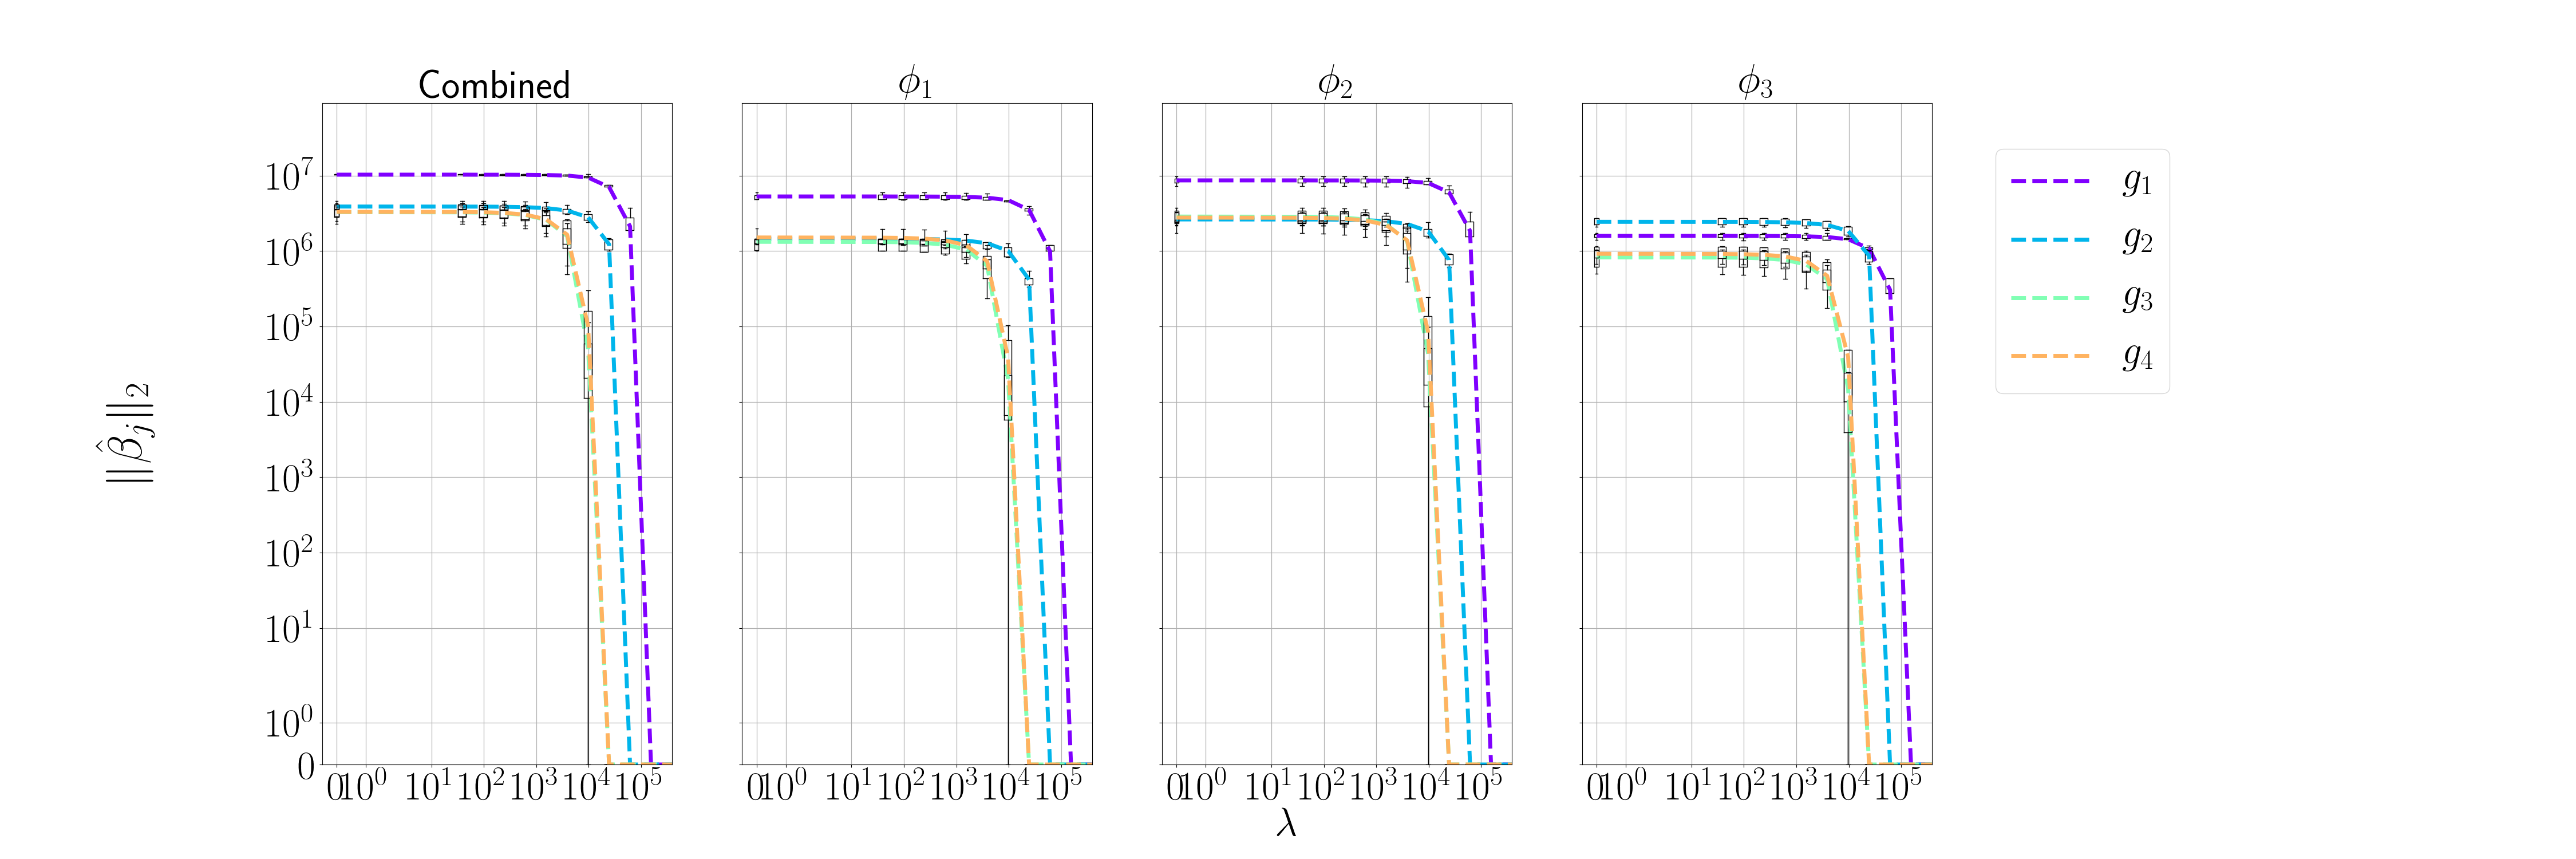
\includegraphics[width=4\picwi,height=1.5\picwi]{../Figures/ethanol/June_27_2019_17_17_08/betassymlogsymlogbeta_paths_n50000nsel100nreps5.png}
\end{tabular}
\caption{\ethdata~ The left panel displays $||\beta_{1:p}||$ as a function of the regularization parameter $\lambda$. The remaining panels display, each for one of the embedding coordinates $\phi_k$, the norm of the vector $\vec(\beta_{i,j,k},\,i=1:n')$. For $\lambda > 10^4$, $\phi_{1,2}$ are explained by $g_1$, while $\phi_3$ is explained by $g_2$. Note that some preference is given to $g_2$ by $\phi_3$, and that this corresponds to the embedding that we see in Figure \ref{fig:molecs}. Axes are linear between $0$ and $1$, and logarithmic above $1$. Error bars summarize the outcomes of the $\omega$ repetitions.
}
\label{fig:mds-ethanol}  
\end{figure}

\paragraph{Malonaldehyde}\label{sec:malonaldehyde}

\begin{figure}[H]
\setlength{\picwi}{0.3\llw}
\begin{tabular}{ccc}
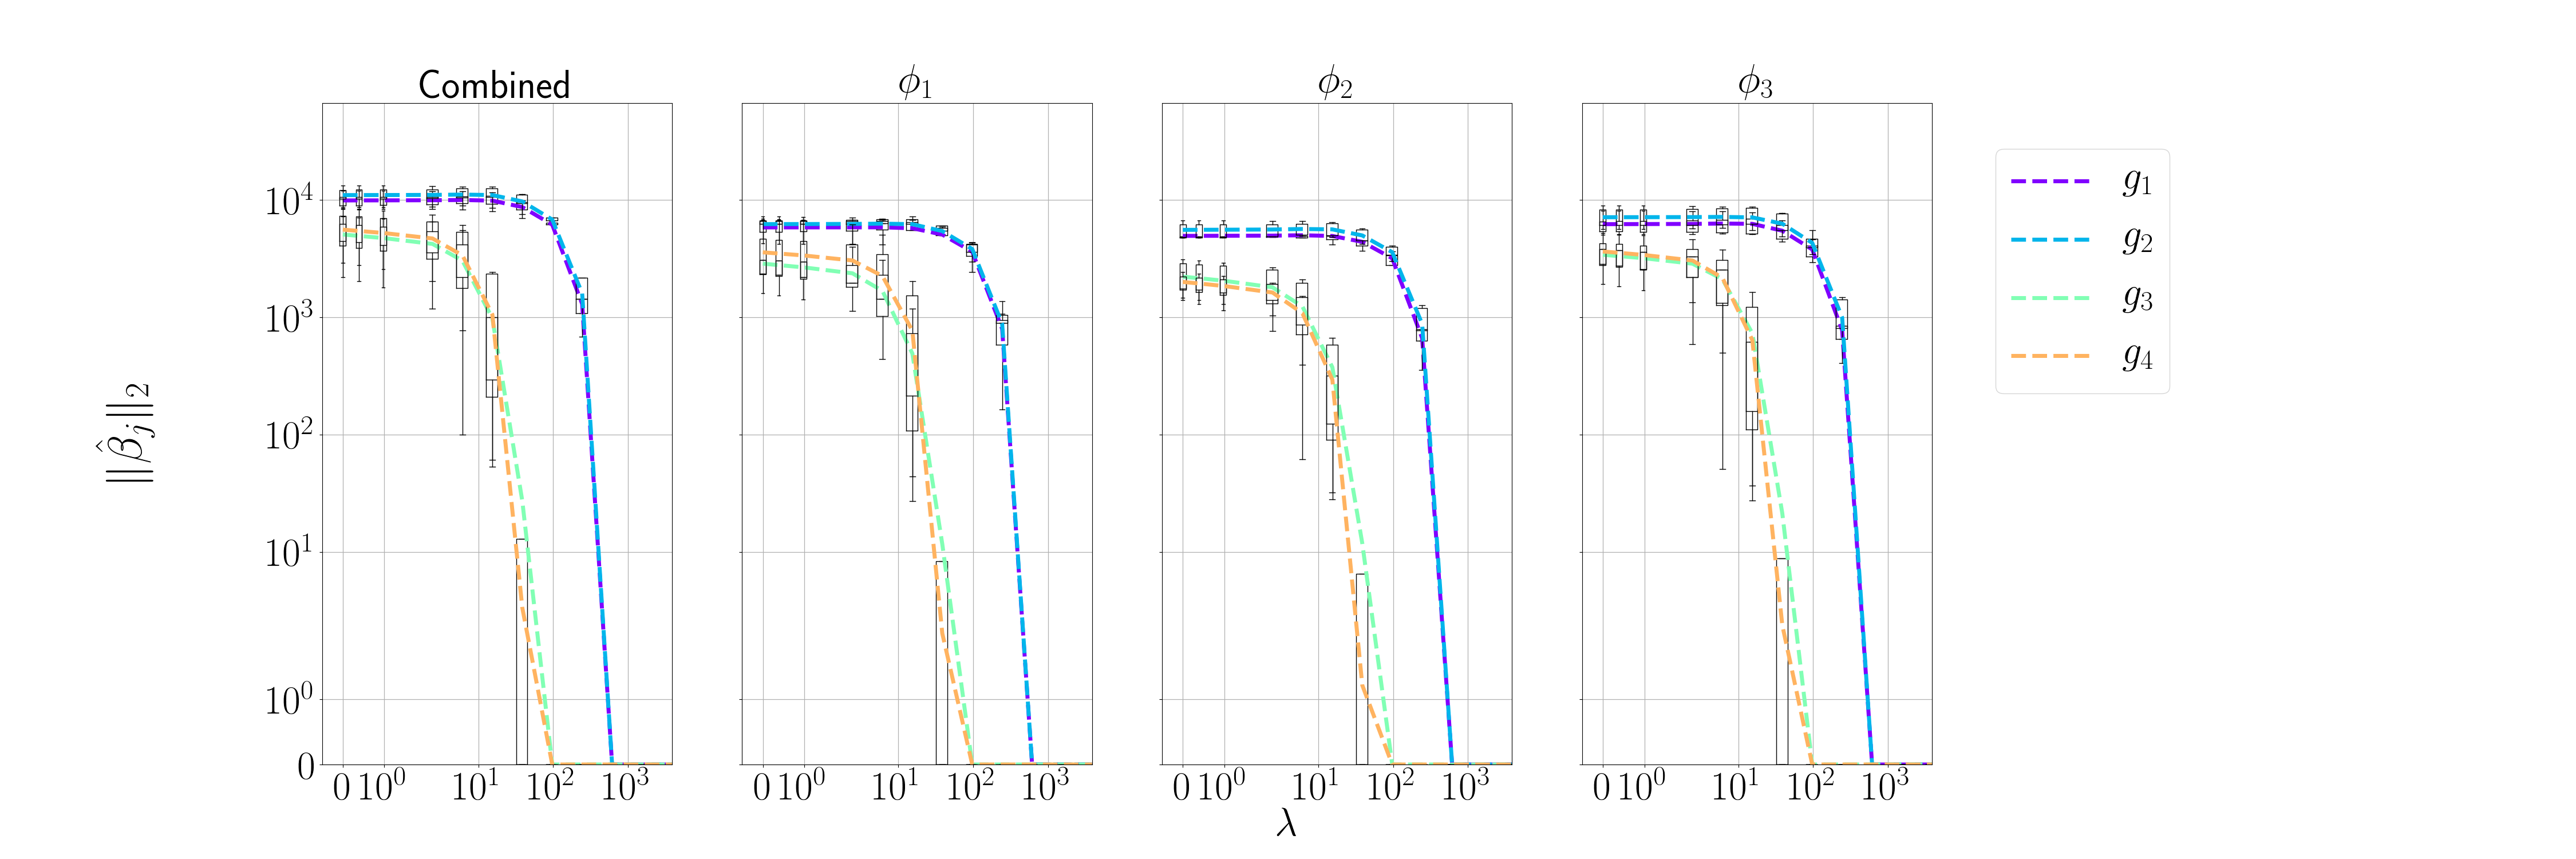
\includegraphics[width=4\picwi,height=1.5\picwi]{../Figures/malonaldehyde/June_27_2019_17_24_21/betassymlogsymlogbeta_paths_n50000nsel50nreps5.png}
\end{tabular}
\caption{\maldata~ The left panel displays $||\beta_{1:p}||$ as a function of the regularization parameter $\lambda$. The remaining panels display, each for one of the embedding coordinates $\phi_k$, the norm of the vector $\vec(\beta_{i,j,k},\,i=1:n')$. For $\lambda > 10^2$, $\phi_{1,2,3}$ are explained by $g_{1:2}$. This corresponds to the embedding that we see in Figure \ref{fig:molecs}. Axes are linear between $0$ and $1$, and logarithmic above $1$. Error bars summarize the outcomes of the $\omega$ repetitions.
\label{fig:mds-malonaldehydel} }
\end{figure}

%Malonaldehyde has a slightly more complex structure than ethanol, with possible p-orbital hybridization between the two oxygen atoms.

Figure \ref{fig:molecs} shows that the estimated manifold is a two-dimensional surface on which bond torsions $g_1$ and $g_2$ vary smoothly. Our dictionary consists of these two torsions, as well as two other dihedral angles. \ouralg~ identifies that $g_1$ and $g_2$ explain the manifold. In contrast to ethanol and rigid ethanol, all coordinates are associated indistinguishably with both functions.

%\mmp{to merge if needed}

\paragraph{Toluene}\label{sec:toluene}
%Toluene is a simple small molecule with one rotational degree of freedom.  P-orbital hybridization keeps the benzene ring and its peripheral hydrogens locked in a planar configuration, while the CH3 methyl group can rotate freely.

Figure \ref{fig:molecs} shows that the estimated manifold is a circle parameterized by the $CH_3$ methyl torsion $g_1$.  Our dictionary consists of this angle, as well as other dihedral angles throughout the molecule. \ouralg~  identifies that $g_1$ explains the manifold, and associates both coordinates with this function. 
 It is easy
to see that the the \dpullalg~maps tangent vectors from the embedding
space back to the correct subspace.

%In contrast to the setting in the previous section, we have no a priori knowledge of the shape of the data manifold. We can visually check that this circle corresponds to a bond torsion of the methyl group.

%\ouralg~ provide a statistically validated alternative to this visual inspection method.
\begin{figure}[H]
\setlength{\picwi}{0.3\llw}
\begin{tabular}{ccc}
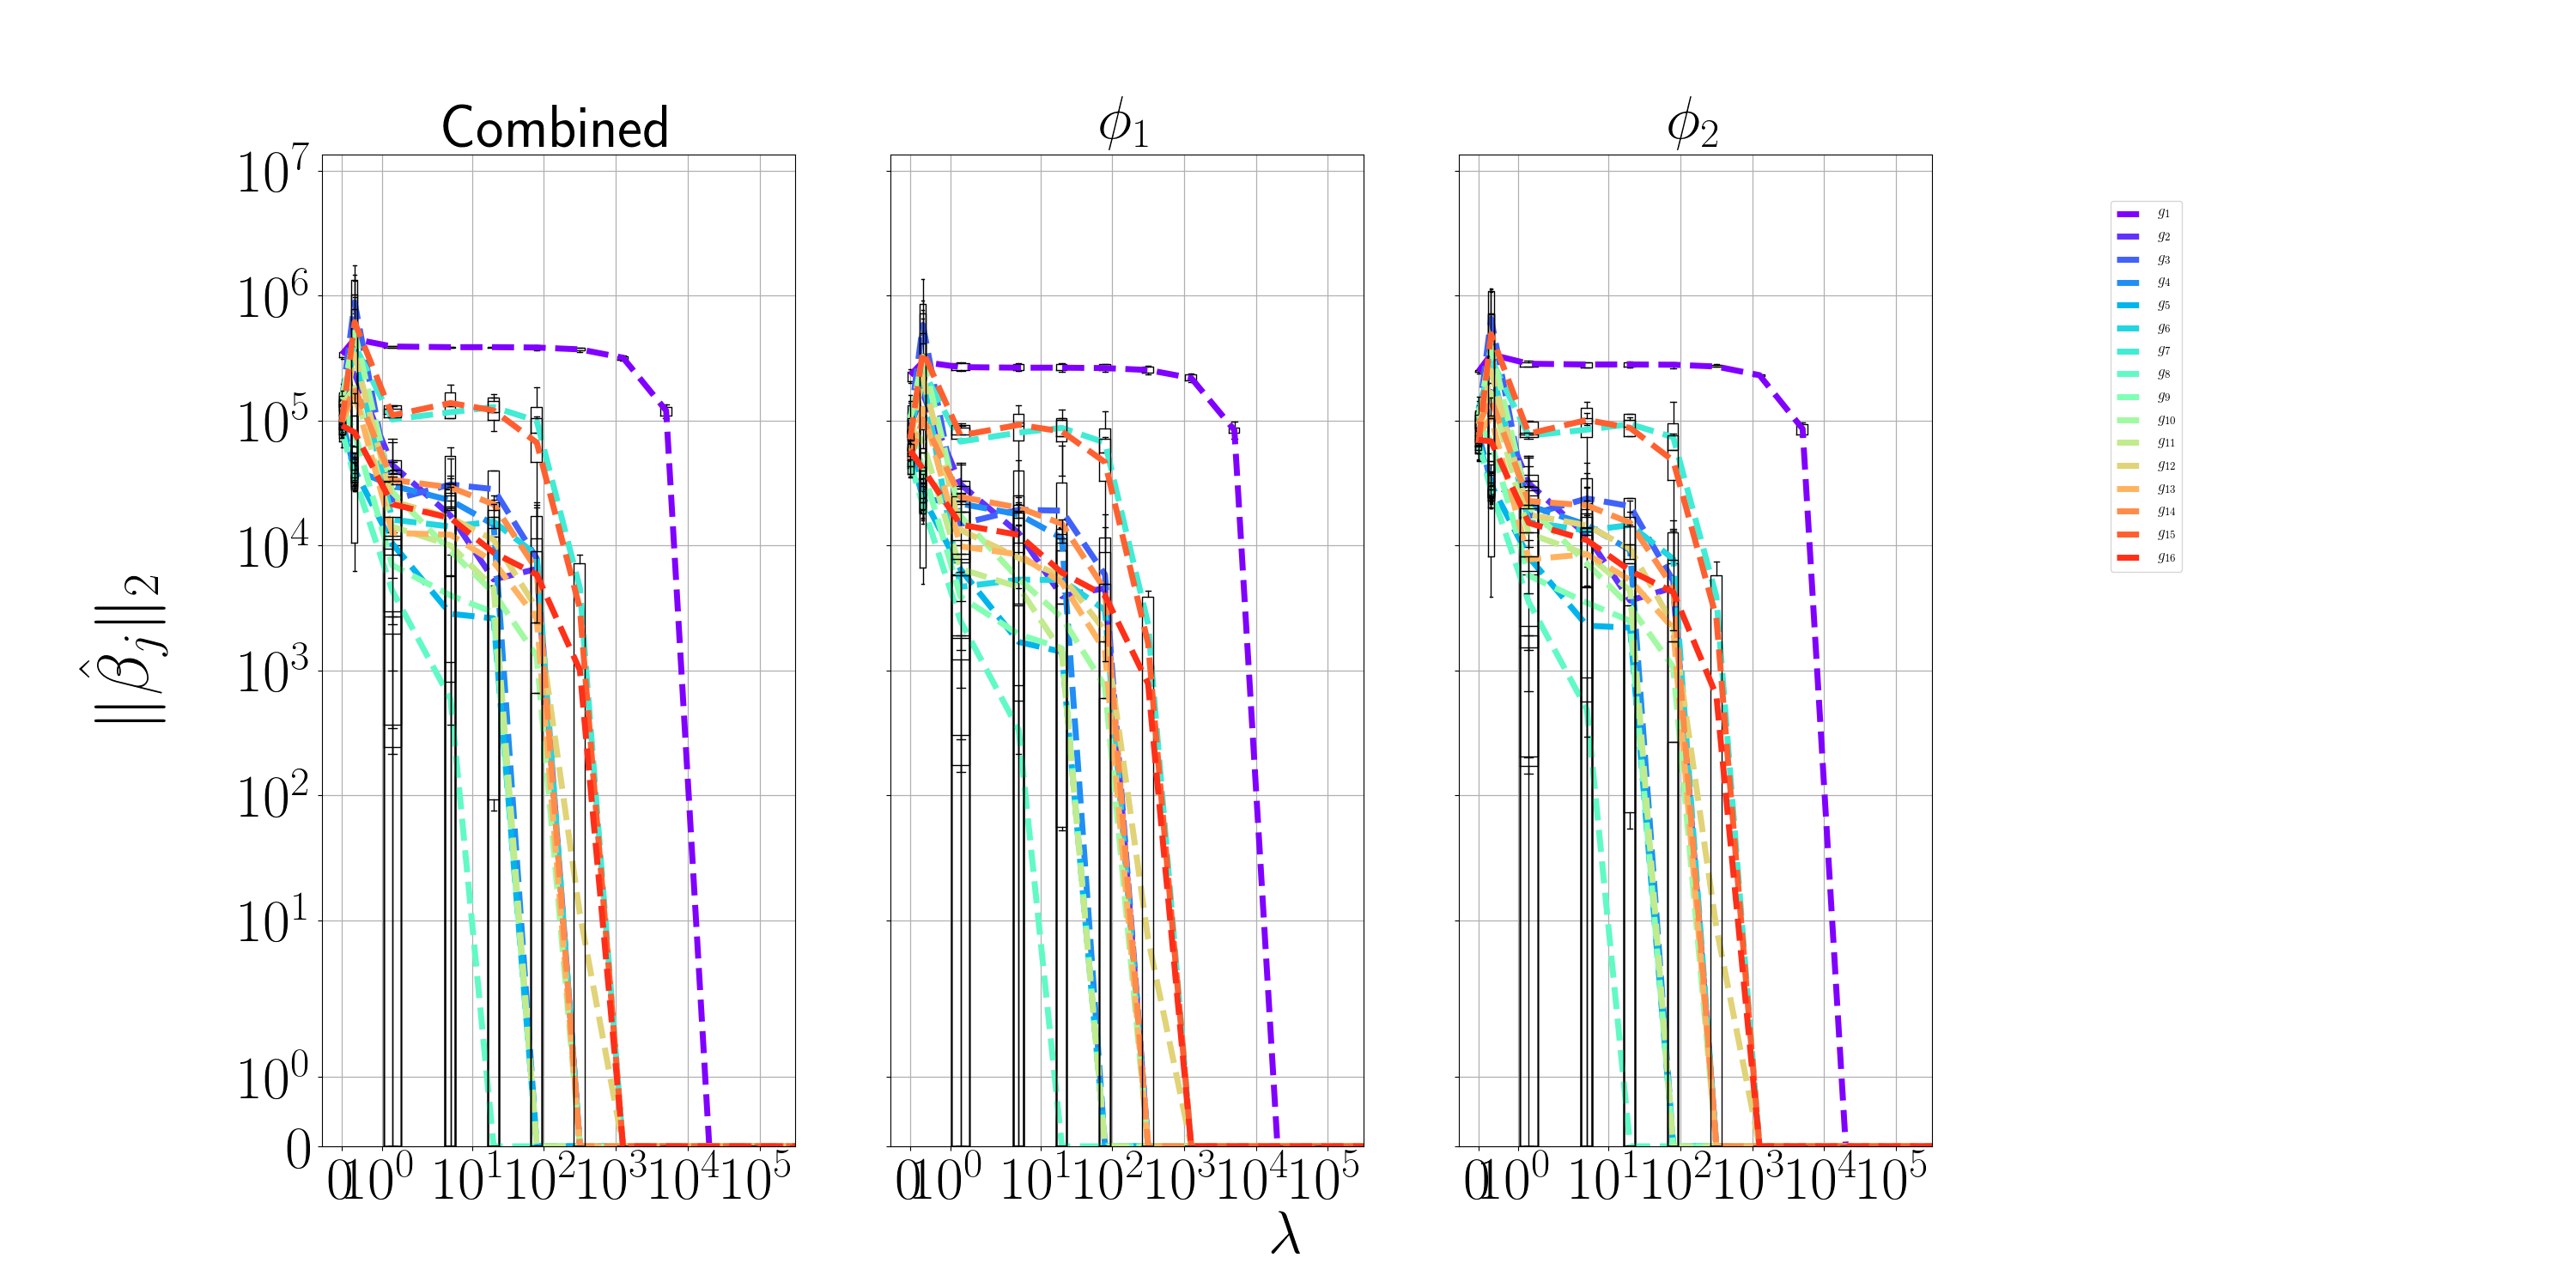
\includegraphics[width=4\picwi,height=1.5\picwi]{../Figures/toluene/June_27_2019_17_17_08/betassymlogsymlogbeta_paths_n50000nsel50nreps5.png}
\end{tabular}
\caption{\toldata~ The left panel displays $||\beta_{1:p}||$ as a function of the regularization parameter $\lambda$. The remaining panels display, each for one of the embedding coordinates $\phi_k$, the norm of the vector $\vec(\beta_{i,j,k},\,i=1:n')$. For $\lambda > 10^3$, $\phi_{1,2}$ are explained by $g_{1}$. This corresponds to the embedding that we see in Figure \ref{fig:molecs}. Axes are linear between $0$ and $1$, and logarithmic above $1$. Error bars summarize the outcomes of the $\omega$ repetitions.
}
\label{fig:mds-toluene}
\end{figure}
\section{Conclusion}
\label{sec:conc}
Both linear and non-linear dimension reduction methods map data to abstract coordinates, derived from agnostic, intrinsic data properties, such as the covariance matrix, in the case of PCA, or the Laplacian, in the case of the Laplacian Eigenmaps algorithm. \ouralg~regresses the abstract coordinate functions on a dictionary $\G$ of functions of the data that have meaning in the domain of the problem. This allows us to  automatically
establish relationships between the learned manifold and domain knowledge. The expert is freed from the tedious work of visually inspecting each possible function $g$ with the manifold coordinates; her expertise is used by specifying covariate functions of the data. The recovered results come with guarantees which can be partially checked in practice. With the obvious simplifications, \ouralg~can also be used to assign explanations to coordinates obtained by PCA. 

The approach of \ouralg~is to reconstruct the
differentials of the manifold coordinates from
differentials of functional covariates. It is robust to
non-linearity in both the algorithm and the covariates. It
requires functions that are smooth, as well as the assumption that the
data lie near a smooth manifold. We estimate the differentials of the
manifold embedding algorithm, but use differentials of functional
covariates that are available analytically. We demonstrate this
approach on {\em Molecular Dynamics (MD)} simulations that generate
high-dimensional point clouds sampled from the configuration space of
a given molecule. Our functional covariates are bond torsions, and the
embedding coordinates display a denoised version of the data. We demonstrate that \ouralg~can detect the torsions upon which these denoised coordinates, and the
denoised manifold embedded within them, depend.



\medskip
\bibliographystyle{alpha}
\begin{small}
\bibliography{../mmp,../materials,../manifolds,../gradients}
\end{small}

\comment{original -proofs merged with unicity. we'll keep this file here because eventually some proofs will be move to the back. There is also a -supplement file that's not used...}
%\input{gradients-nips18-proofs}

\appendix
%\section{Appendices}
\label{sec:appendix}
%\subsection{Appendix A}
%\label{app:md-data}

%We begin with $n$ data points of dimension $3N_a$ corresponding to the Euclidean coordinates of each atom within the molecule. To respect rotational, dilation, and translational molecular symmetry, we transform these $3N_a$ coordinates into $D= 3 {N_a \choose 3}$ angles of atomic triplets. These coordinates are then used to learn an embedding in m coordinates.

%\ouralg~ is applied to a randomly chosen subset of $n'$ using $p$ dictionary functions, and this process is repeated reps number of times. Importantly, since our angular coordinates are redundant, we necessarily adapt \ouralg~ to the shape space $\Sigma_3^{N_a}$. Embedding and tangent space estimation is done in dimension $D$, while normalization and regression is done in the shape space of dimension $3N_a - 7$. In all experiments, we assume that manifold dimension $d$ has already been estimated. The full specifics of our MD data analytics pipeline are in Appendix \ref{app:md-data}.


%This section describes details of the data processing. Sections \ref{sec:}--\ref{sec:} describes the experimental results. In both 'real' and synthetic MD experiments our data processing procedure procedure is as follows. \mmp{samples, transformatin and preprocessing, manifold embedding -- what alg and params, manifold lasso}


%We consider a molecular position to be a collection of $N_a$ points in $\mathbb R^3$, where $N_a$ is the number of atoms in the molecule. A molecular trajectory consists of a set or sequence of molecular positions. We apply a manifold learning algorithm to identify the low-dimensional manifold these trajectories are sampled around. We then apply \ouralg~  to perform sparse functional support recovery for the embedding coordinates. In particular, we identify an explanation of this manifold in terms of bond torsions.
%\subsection{Appendix B}

\section{The shape space}
\label{app:shape-space}
Here we formally define the shape space, and show how to obtain the gradient of a function $g_j$ of a molecular configuration, at a non-singular point, in the tangent bundle of this space.

We define the \textit{shape space}
\begin{align*}
 \Sigma_3^{N_a} = \rrr^{3N_a} \slash (E(3) \times \rrr^+ ),
\end{align*}
where $E(3)$ is the three dimensional Euclidean group composed of rigid rotations and translations in $\rrr^3$, and $\rrr^+$ is a dilation factor relative to the mean position of the $N_a$ atoms. That is, $\Sigma_3^{N_a}$ is the space of positions of $N_a$ atoms in $\rrr^3$ with equivalences given by translation, rotation, and dilation. Away from singularities of measure zero, $\Sigma_3^{N_a}$ is a Riemannian manifold \citep{Le1993-mg, addicoatcollins:2010}.

Denote the Euclidean coordinates of $ \rrr^{3N_a}$ by $r$, and the Euclidean position of each data point by $r_i$. Recall that we compute $a_i = a(r_i)$ for $i \in 1, \dotsc n$, where $a$ is the vector-valued function
\begin{align*}
a: \rrr^{3N_a} \to \rrr^{3{N_a \choose 3}}
\end{align*}
that computes the angles formed by all triples of atoms in the molecule. This angular featurization of the data respects the symmetries of the shape space, and embeds the shape space.
%\label{sec:test}
We compute bases for the tangent spaces of $\Sigma_3^{N_a}$ as follows. For every analyzed point $i$, we compute the matrix of partial derivatives, also known as the Wilson B-matrix,
\begin{align*}
W_i = \frac{\partial a}{\partial r} (r_i) \in \mathbb R^{3N_a \times \mathbb R^{3 {N_a \choose 3}}}.
\end{align*}
Note that $W_i$ is the transpose Jacobian of $a$. 
%Away from singularities of measure zero, we can compute the tangent space of $\Sigma_3^{N_a}$ with respect to its embedding in $\rrr^{3{N_a \choose 3}}$. By projecting onto $T \Sigma_3^{N_a}$, we remove the issue of angular redundancy in the sense that all gradients of the same torsion are equivalent after projection, regardless of which angles were used to compute the torsion. Thus, normalization with respect to these gradients is well-defined.
This computation is done using automatic differentiation. We then calculate the reduced Singular Value Decomposition
\begin{align*}
W_i = U_i \Lambda_i V_i^T
\end{align*}
where  $\Lambda_i$ is a diagonal matrix of dimension $3N_a - 7$, containing the non-zero singular values of $W_i$. A deductive explanation for the rank of $W_i$ is that translation, rotation, and dilation correspond to a total of 7 degrees of freedom. The $3N_a - 7$ corresponding singular vectors in $V_i$ are a basis for the tangent space $\T_i  \Sigma_3^{N_a}$ in $\rrr^{3 {N_a \choose 3}}$ \citep{addicoatcollins:2010}. Let $a_i = a(r_i)$ for $i \in 1, \dotsc n$. We can then project
\begin{align*}
%\grad_{\Sigma_3^{N_a}} g_j (a_i) &= V_i V_i^T \nabla_{\mathbb R^{3 {N_a \choose 3}}} g_j (a_i),
\grad_{\Sigma_3^{N_a}} g_j (a_i) &= V_i V_i^T \nabla_{a} g_j (a_i),
\end{align*}
where $\nabla_a g_j (a_i)$ is obtained with automatic differentiation using a close-form expression for the dictionary function in the angular coordinates $a$ of $\rrr^{3 {N_a \choose 3}}$, and $\grad_{\Sigma_3^{N_a}}$ is the gradient on the shape manifold in the angular coordinates.

Recall that we apply Principal Component Analysis to the angular features matrix  $a_{1:n} \in \rrr^{n \times D}$. To perform PCA, we use Singular Value Decomposition:
\begin{align*}
a_{1:n} = M \Pi N^T.
\end{align*}
Denote by $P$ the matrix formed with the first $D$ columns of $N$; $P$ projects the angular features into a lower dimension space that reduces redundancy while capturing the vast majority of the variability. \comment{For this paper, we use $D = 50$.} That is, \\
\begin{align*}
\xi_i &= a_i P,\;\text{for}\; i=1,\ldots n.
\end{align*}
The gradient of $g_j$ with respect to coordinates $\xi$ are given by
\begin{align*}
\grad_{\xi} g_j (\xi_i)= P^T \grad_{\Sigma_3^{N_a}} g_j (a_i).
\end{align*}
We use $\grad_{\xi} g_j (\xi_i)$ as $\nabla_{\xi} g_j (\xi_i)$ in \ouralg.
%We then normalize with respect to $\grad_{\xi} g_j$.
%\begin{align*}
%\grad_{\xi} g_j (\xi_i) =\frac{ \grad_{PCA} g_j (\xi_i)}{\sum_{i=1}^n \| \grad_{\xi} g_j (\xi_i) \|_2}
%\end{align*}
%Finally, we compute
%\begin{align*}
%TM^T \grad_{\xi} g_j = \grad_{M} g_j.
%\end{align*}
%We utilize $\grad_{\Sigma_3^{N_a}} \phi_m$ and the normalized version of $\grad_{\Sigma_3^{N_a}} g_j$ as our functional variables in group lasso.

%That is, $ respect this symmetry, we featurize each configuration in terms of the angles of the triangles formed by all combinations of three atoms, i.e. as an element of $\rrr^D$, where $D = 3{N_a \choose 3}$. The manifold learning algorithm is then applied to this representation of the data.

%In order for our normalization procedure to be well-defined, it is necessary to consider the dictionary functions as functions of the manifold $\Sigma_3^{N_a}$ rather than $\rrr^D$. This is because $\rrr^D$ is an overparameterized space, and so dictionary functions do not have a unique gradient field. To remedy this, we project any suitable gradient field computed in $\rrr^D$ onto the tangent bundle of $\Sigma_3^{N_a}$. This projection is based on the idea that $\Sigma_3^{N_a}$ is a rank $3N_a - 7$ space inside of $\rrr^D$, and amounts to identifying the tangent bundle of $\Sigma_3^{N_a}$ using differential constraints between the angles. Although this space has singularities, they are of measure zero, and are not encountered in practice. Note that we cannot apply an embedding algorithm to $\Sigma_3^{N_a}$ directly, since this is not a Euclidean space, and nearest neighbor search is not guaranteed to be work, although in principle we could search in $\rrr^D$ and compute geometry with respect to $\Sigma_3^{N_a}$. Also note that the metric we implicitly use for $\Sigma_3^{N_a}$ is inherited from the angular representation, therefore that our shape space is not isometric to that of \cite{le}.

%\mmp{Shape space thoughts> Let $a$ be the angle coordinates, $\xi$ be the coordinates obtained from $a$ after PCA, and $r$ be the Cartesian atom coordinates. We have that $\xi=\sqrt{\Sigma}U^Ta$, where $Cov(a)=U\Sigma U^T$, and $\Sigma$ has rank $D$. Then, $\fracpartial{\xi}{r}=\sqrt{\Sigma}U^T\fracpartial{a}{r}$, with $\fracpartial{a}{r}$ obtained by automatic differentiation. We calculate the SVD of $\fracpartial{\xi}{r}$,
%\[
%\fracpartial{\xi}{r}\;=\;U_\xi\Lambda_\xi V_\xi^T
%\]
%where  $\Lambda$ contains $3N_a - 7$ non-zero eigenvalues. The first $3N_a - 7$ eigenvectors in $U_\xi$ are a basis for the tangent space $\T \tilde \Sigma_3^{N_a}$ embedded in $\rrr^D$. We can then project the gradients of $g_j$ obtained by automatic differentiation w.r.t. $r$ onto this tangent space by
%\[
%\grad_\xi g_j\;=\;U_\xi\nabla_r g_j
%\]
%We use $\grad_\xi g_j$ in place of $\nabla_\xi g_j$ in the \ouralg~algorithm.
%}

%\skcomment{I believe it is a different idea. The core of the idea may be preferable to what we are currently doing, but I am not sure.  Here is a major point of confusion for me (using your notation): 
%$\frac{\partial \xi}{\partial r} \in \mathbb R^{3N_a \times  D}$
%so if $\frac{\partial \xi}{\partial r} = U_\xi \lambda_\xi V_\xi^T$
%then the first $3N_a - 7$ singular vectors of $U_\xi$ form a matrix $\tilde U_\xi \in \mathbb R^{3N_a \times 3N_a-7}.$
%Then we get $\tilde U_\xi^T \nabla_r g_j \in \mathbb R^{3N_a-7} \neq \mathbb R^D.$
%So I don't think the dimensions of the vectors are what we are looking for.
%There may be a similar approach taking advantage of the fact that $\frac{\partial \xi}{\partial r}$ is rank $3N_a-7$.}

\begin{figure}[H]
\setlength{\picwi}{0.3\llw}
\begin{tabular}{cc} 
%A
%\includegraphics[width=1.5\picwi,height=2\picwi]{rigapp.png}
% &
%B
%\includegraphics[width=1.5\picwi,height=2\picwi]{rigbpp.png} \\
%\multicolumn{2}{c}{
%C
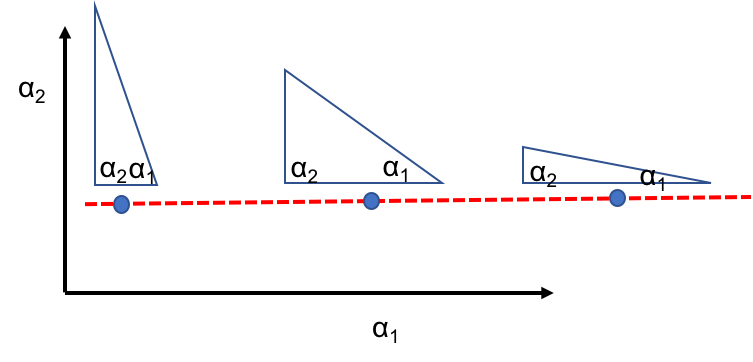
\includegraphics[width=4\picwi,height=2\picwi]{../Figures/righttriangles.png}
\end{tabular}
\caption{\label{fig:shapespace} This diagram shows a simplified representation of the neighborhood of a point in the shape space $\Sigma_2^3$. Up to rotation, dilation, and translation, the shape of a triangle is determined by two angles, so we can see that this is a two-dimensional space.  The diagram represents the logarithmic map of a region of $\Sigma_2^3$, with the red line indicating the logarithmic map of the subspace of right triangles, in a coordinate system given by $\alpha_1$ and $\alpha_2$, two angles in the triangle.
}
\end{figure}

%<<<<<<< HEAD


%\subsection{Appendix B}
%\label{app:function-dependency-data}

%\subsection{Appendix C}
%\label{app:embedding-algorithm}
%=======
%At every data point, denote the basis of $D$ redundant angular variables by $z$, and the $3N_a$ Euclidean coordinates of the molecule by $x$. For every analyzed point, we compute the matrix of partial derivatives, also known as the Wilson B-matrix,
%\begin{align*}
%W = \frac{\partial z}{\partial x}.
%\end{align*}
%When then perform a singular value decomposition
%\begin{align*}
%W = U \Lambda U^T
%\end{align*}
%where  $\Lambda$ contains $3N_a - 7$ non-zero eigenvalues. A deductive explanation for the rank of $W$ is that translation, rotation, and dilation correspond to a total of 7 degrees of freedom. The first $3N_a - 7$ eigenvectors in $U$ are a basis for the tangent space $T \tilde \Sigma_3^{N_a}$ embedded in $\rrr^D$. We can then project
%\begin{align*}
%\grad_{\Sigma_3^{N_a}} g_j &= U \grad_D g_j \; \text {and} \\
%\grad_{\Sigma_3^{N_a}} \phi_m &= U \grad_{D} \phi_m. \text{\mmp{we don't do this, right?}}
%\end{align*}
%We utilize $\grad_{\Sigma_3^{N_a}} \phi_m$ and the normalized version of $\grad_{\Sigma_3^{N_a}} g_j$ as our functional variables in group lasso.

%\section{Function dependency data}
%\label{app:function-dependency-data}
%\mmp{what's this?}
%\section{Diffusion Maps embedding algorithm}
%\label{app:embedding-algorithm}
%>>>>>>> cdd11cc241cb349bd809fb501520a4e91935eb18

\section{Torsion Computation}
\label{app:dictionary-details}

For molecular dynamics analyses, our dictionary $\G$ consists of bond torsions, which are computed from angles, and whose gradients are obtained using automatic differentiation in Pytorch.
  Diagrams \ref{figtab:eth} -  \ref{figtab:mal} show the identities of the torsions input as functional dictionaries to \ouralg.  Torsions experimentally validated to explain the data manifold are marked with a *.
  
\begin{table}[H]
\begin{tabular}{cc}
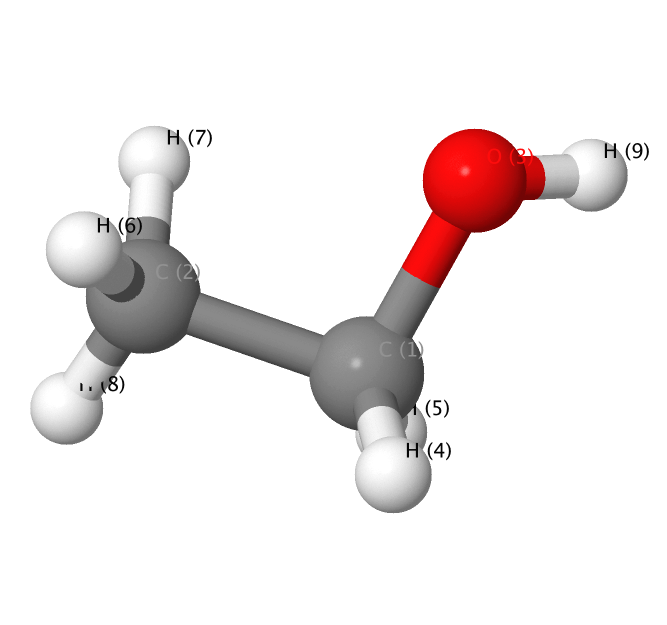
\includegraphics[scale=0.25,valign=m]{../Figures/ethanol/ethanol.png}
&
\begin{tabular}{ | c | c | } 
\hline
\G \# & Atom \# s \\
\hline
$g_1*$ & [7,2,1,5]\\
\hline
$g_2*$ & [5,1,3,9] \\
\hline
$g_3$ & [8,7,6,2] \\
\hline
$g_4$ & [4,1,3,5]\\
\hline
\end{tabular}
\end{tabular}
\caption{Diagram of ethanol and identities of bond torsions.  Torsions are the angle of the planes formed by the first three and last three atoms. Torsions experimentally validated to explain the data manifold are marked with a *.}
\label{figtab:eth}
\end{table}
%\clearpage

%\FloatBarrier
%\paragraph{Toluene}

\begin{table}[hbt!]
\begin{tabular}{cc}
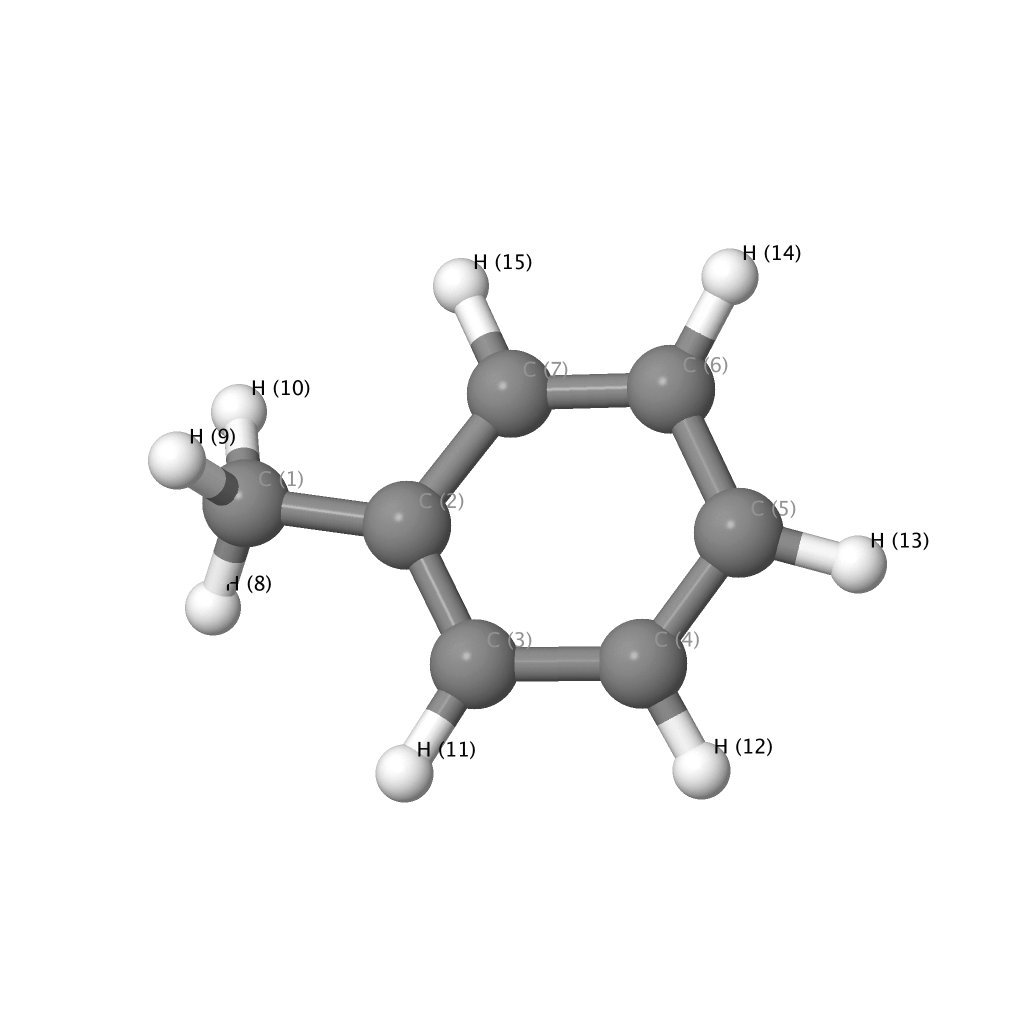
\includegraphics[scale=0.25,valign=m]{../Figures/toluene/toluene.png}
&
\begin{tabular}{ | c | c | } 
\hline
Torsion \# & Atom \# s \\
\hline
$g_1*$ & [10,1,2,3]\\
\hline
$g_2$ & [1,2,3,4]\\
\hline
$g_3$ &[2,3,4,5]\\
\hline
$g_4$ & [3,4,5,6]\\
\hline
$g_5$ &[4,5,6,7]\\
\hline
$g_6$ &[5,6,7,2]\\
\hline
$g_7$ &[6,7,2,1]\\
\hline
$g_8$ & [1,2,4,12] \\
\hline
$g_9$  & [11,3,5,13]  \\
\hline 
$g_{10}$ & [12,4,6,14] \\
\hline 
$g_{11}$ & [13,5,7,15] \\
\hline 
$g_{12}$ & [11,3,7,14] \\
\hline 
$g_{13}$ & [1,2,6,14] \\
\hline 
$g_{14}$ & [12,4,7,15] \\
\hline 
$g_{15}$ & [13,5,2,1] \\
\hline 
$g_{16}$ & [11,3,6,14] \\
\hline
\end{tabular}
\end{tabular}
\caption{Diagram of toluene and identities of bond torsions.  Torsions are the angle of the planes formed by the first three and last three atoms. Torsions experimentally validated to explain the data manifold are marked with a *.}
\label{figtab:tol}
\end{table}

%\paragraph{Malonaldehyde}


\begin{table}[hbt!]
\begin{tabular}{cc}
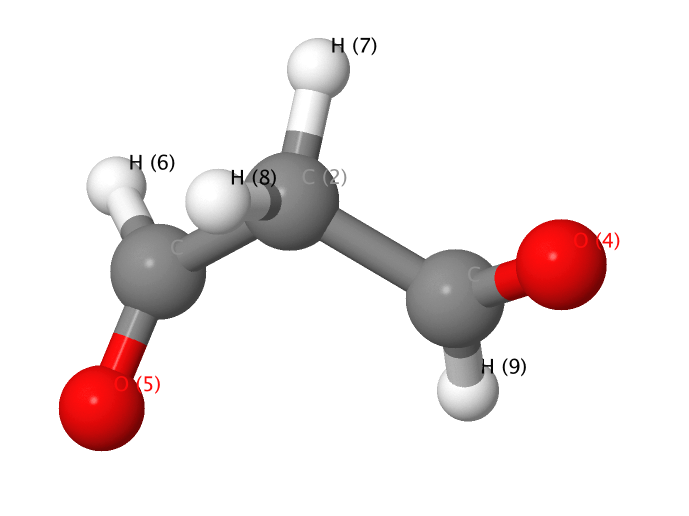
\includegraphics[scale=0.25,valign=m]{../Figures/malonaldehyde/malonaldehyde.png}
&
\begin{tabular}{ | c | c | } 
\hline
$\G$ \# & Atom \# s \\
\hline
$g_1*$ & [5,1,2,3]\\
\hline
$g_2*$ &[1,2,3,4]\\
\hline
$g_3$ &[4,3,2,9]\\
\hline
$g_4$ &[5,1,2,6] \\
\hline
\end{tabular}
\end{tabular}
\caption{Diagram of malonaldehyde and identities of bond torsions.  Torsions are the angle of the planes formed by the first three and last three atoms. Torsions experimentally validated to explain the data manifold are marked with a *.}
\label{figtab:mal}
\end{table}

%}
%\end{figure}


\end{document}
